%%%%%%%%%%%%%%%%%%%%%%%%%%%%%%%%%%%%%%%%%%%%%%%%%%%%%%%%%%%%%%%%%%%%%%%%%%%%%
%%
%% This file provides a template that can be used in concert with the
%% ohio-etd class to generate an electronic thesis or dissertation which
%% meets the formatting requirements at Ohio University.
%%
%% To use the template, copy this file (template.tex) and ohio-etd.cls into
%% the same directory and edit this template as required.  Reference
%% ohio-etd.pdf for additional instructions on using this class.
%%
%%%%%%%%%%%%%%%%%%%%%%%%%%%%%%%%%%%%%%%%%%%%%%%%%%%%%%%%%%%%%%%%%%%%%%%%%%%%%


%% Load the class.  Available options are: numbered, pdftex, cmfont,
%% singlespacetables, draft, 11pt, 12pt, leqno, and fleqn

\documentclass[numbered,pdftex]{ohio-etd}
\usepackage{cite}
\usepackage{notoccite}
\usepackage{bbding}
\usepackage[utf8]{inputenc}

\usepackage{array}




\usepackage[normalem]{ulem}

\usepackage{ragged2e}
\usepackage{verbatim} 
\usepackage{hyperref}
\usepackage{flafter}
\usepackage{color,soul} % Highlighting 
\usepackage{subfigmat}

\usepackage{float} % In-text figs
\usepackage{varioref}%  smart page, figure, table, and equation ref
\usepackage{graphicx} % Include graphics
\usepackage{epstopdf} % Figure type .eps to .pdf
\usepackage{wrapfig} % Figures in text
\usepackage{listings}
\usepackage{color} %red, green, blue, yellow, cyan, magenta, black, white

%\floatstyle{boxed}
%\restylefloat{figure}


\definecolor{mygreen}{RGB}{28,172,0} % color values Red, Green, Blue
\definecolor{mylilas}{RGB}{170,55,241}

\newcolumntype{L}[1]{>{\raggedright\let\newline\\\arraybackslash\hspace{0pt}}m{#1}}
\newcolumntype{C}[1]{>{\centering\let\newline\\\arraybackslash\hspace{0pt}}m{#1}}
\newcolumntype{R}[1]{>{\raggedleft\let\newline\\\arraybackslash\hspace{0pt}}m{#1}}


%% Other packages that may be of use.  Delete or comment out (using a
%% percent sign in the first column) if they are not desired.  Reference
%% the corresponding documentation for more information on how to use these
%% packages.

%\usepackage[square,sort&compress,numbers]{natbib} % Provides formatting for
                                                  % citations
\usepackage{textcomp} % Provides math symbols that can be used in text mode
\usepackage{amssymb}  % Provides additional AMS math symbols.  Note that
                      % amsmath is loaded as part of the ohio-etd class
\usepackage{bm}       % Provides bold-faced math symbols
\usepackage{booktabs} % Provides improved table formatting
\usepackage{dcolumn}  % Provides table columns aligned at decimal points
\usepackage{multirow} % Provides table elements spanning multiple rows
\usepackage{graphicx} % Standard package to incorporate graphics
\usepackage[printonlyused]{acronym} % Provides a method for incorporating
                                    % acronyms and building an acronym list
\usepackage{relsize}
\usepackage{amsmath} % Inserting Equations

\graphicspath{{figures/}} % Allows graphics files to be stored in a
                          % separate directory
\usepackage{fancyref}




%% Required front matter definitions

\degree    {MS}              % MS, MA, MCTP, or PhD
\graduation{August}{2018}    % May, August, or December 

\title     {An Optimized Circulating Vector Field Obstacle Avoidance Guidance for Unmanned Aerial Vehicles}
\author    {Garrett S.}{Clem} 

\advisor   {Jay P. Wilhelm}{Assistant Professor of Mechanical Engineering}
\dean      {Dennis Irwin}{Dean, Russ College of Engineering and Technology }
\program   {Mechanical Engineering}            % e.g. Electrical Engineering
\department{Department of Mechanical Engineering} % e.g. School of Electrical Engineering 
                                    %      and Computer Science
\college   {Russ College of Engineering and Technology}   % e.g. Russ College of Engineering and
                                     %      Technology
\abstract  {Unmanned Aerial Vehicles (UAVs) conventionally navigate by following a series of pre-planned waypoints. When encountering an obstacle in flight, such as no-fly zones or other aircraft, the vehicle's path or waypoints may need to be re-planned. Waypoint guidance can be used to avoid obstacles, which are typically generated off-line and relayed to the UAV requiring active communications. Vector Fields (VFs) that are generated based on a desired path can provide guidance around a newly discovered obstacle without the need for a re-plan. VF convergence and circulation components were optimized to minimize deviation from a desired path when guiding around a circular obstacle. Results indicated that the developed VF obstacle avoidance optimizer provides similar path deviation performance as waypoints without the need for re-planning. Lookup tables for GVF circulation and decay radius were constructed allowing for real time obstacle avoidance without the need to re-plan mission waypoints. Experimental flight tests were conducted using a indoor quadcopter with imposed turn rate constraints, emulating a fixed wing UAV. Deviation from the planned path for simulation and experimentation were compared.}
 

%% Optional front matter definitions.  Delete or comment out if not needed

% \coadvisor {Coadvisor's Full Name}{Coadvisor's Full Title}

\dedication{In memory of Jack Clem}
%
\acknowledgments{Throughout my graduate studies I have had the privilege of working with many unique and sophisticated people. First and foremost, I would like to thank my advisor Dr. Jay Wilhelm for his seemingly limitless academic support. Without his leadership this work would not have been completed. I would like to also thank my committee members, Dr. Casbeer, Dr. Williams, and Dr. Uijt de Haag for their time, suggestions, and stimulating discussions in regards to the contents of this research.  \\
To my first lab colleague, Gina, your mentoring and friendship were invaluable and I cannot see myself completing this program without  your support and humor. Hunter and Travis, your assistance with debugging the control software was vital to the success of this project. My roommates, Sean, Justin, and Jacob, you all provided welcome distractions. To my mother, who I grew closer with over the past few years, this is for you. Lastly, I would like to thank my best friend Emily whose love and support constantly reminded me why I continued my education to better myself. 
}
%% If you prefer to provide "acknowledgements" instead (note the added "e"
%% between the "g" and the "m") then add the "e" in the macro name so that
%% it reads "\acknowledgements".}

%% Additional "lists" can be added to the end of the front matter using the
%% \addlistof macro.  For example:
\addlistof{Symbols}{\begin{tabbing}
  XXXXXXXXXXXX \= \kill% this line sets tab stop
  \\
  
  $\dot{\theta} $ \> UAV maximum turn rate [deg/s] \\
$\overrightarrow{X} $ \> UAV position [m] \\
$t$ \> time [s] \\
$t$ \> time [s] \\
$\overrightarrow{U} $ \> UAV velocity [m/s] \\
$\theta$ \> UAV heading [deg] \\
$dt$ \> Discrete time step [s] \\
$\overrightarrow{R}$ \> Potential Field heading guidance vector  [deg] \\
$\overrightarrow{F}_t$ \> Potential Field artificial attractive force [-] \\
$(x_t,y_t)$ \> Potential Field goal position [m] \\
$d_t$ \> Potential Field range to goal from robot [m] \\
$\overrightarrow{F}_{i,j}$ \> Potential Field obstacle artificial force [-] \\
$(x_i,y_j)$ \> Potential Field obstacle cell position [m] \\
${i,j}$ \> Potential Field obstacle cell index [-] \\
$F_{cr}$ \> Potential Field constant repulsive artificial force [-] \\
$W$ \> Potential Field vehicle width [m] \\
$C_{i,j}$ \> Potential Field cell certainty [-] \\
$d_{i,j}$ \> Potential Field range to cell center [m] \\
$\chi^d$ \> Lyapunov guidance vector [deg] \\
$\chi^{\inf} $ \> Lyapunov course approach angle [deg] \\
$y$ \> UAV's lateral distance to path [m] \\
$\bar{k}$ \> Lyapunov transition constant [-] \\
$\psi$ \> UAV angular position around loiter circle [deg] \\
$r$ \> Radius of circular path [m] \\
$d$ \> Range to path or obstacle center [m] \\
$n$ \> Number of spatial dimensions [-] \\
$q$ \>Spatial dimension set  [-] \\
$\alpha_i(x_1,x_2,...x_n,t)$ \> Implicit surface function [-] \\
$\overrightarrow{V}$ \> Guidance vector [deg] \\
$G$ \>Convergence weight  [-]  \\
$H$ \>Circulation weight  [-] \\
$L$ \>Time-varying weight [-] \\
$\overrightarrow{V}_{conv}$ \> Convergence vector  [deg] \\
$\overrightarrow{V}_{circ}$ \> Circulation vector  [deg] \\
$\overrightarrow{V}_{tv}$ \> Time varying vector   [deg] \\
$M$ \>Gradient matrix [-] \\
$a$ \>Velocity column vector [-] \\
$\overrightarrow{V}_p$ \> Path following guidance  [deg] \\
$\overrightarrow{V}_o$ \> Obstacle avoidance guidance  [deg] \\
$P$ \>Obstacle field decay weight [-]  \\
$R$ \> Obstacle field decay edge  [-] \\
$\delta$ \> Straight target path angle  [deg] \\
$||\bullet||$ \> Vector magnitude [] \\
$x_c$ \>  Obstacle x position [m] \\
$y_c$ \>  Obstacle y position [m] \\
$\bar{x}$ \> x range to obstacle [m] \\
$\bar{y}$ \> y range to obstacle [m] \\
$r_o$ \> Obstacle radius [m] \\
$m$ \> Obstacle radius multiplier [-] \\
$k$ \> Decay radius multiplier [-] \\
$\theta_r$ \> UAV turning radius [m] \\
$\gamma$ \> Path deviation cost function [-] \\
$tf$ \> Time final [-] \\
$\bar{\gamma}$ \> Path deviation cost function with obstacle penalization [-] \\
$j(x,y)$ \> Obstacle penalization function [-] \\
  
  
  
  
  

 \end{tabbing}}
%% Note that the command "\input{symbols}" can be used if the symbol list is
%% contained in a separate file called "symbols.tex"}

\addlistof{Acronyms}{
\begin{tabular}{lll}
&  & \\
UAV & Unmanned Aerial Vehicles & \\
VF & Vector Field & \\
UAS & Unmanned Aerial System  & \\
VFF & Virtual Force Field  & \\
TPLVF & Tangent Plus Lyapunov Vector Field & \\
RRT* & Optimal Rapid Radom Trees & \\
DT  & Delauny Triangulation & \\
GVF & Gradient Vector Field & \\
 
\end{tabular}}


%% Use "\input{acronyms}" if the acronym list is in a separate file called
%% "acronyms.tex".  Note that the formatting generated by the acronym package
%% can be forced into singlespaced text by inserting "\setlength\itemsep{0pt}
%% \setlength\parskip{0pt}" into the "acronym" environment.} 

%% For documents created by government employees as part of their
%% employment.  The wording of the disclaimer can be specified using an
%% option.  See the documentation for more information.

% \govtdisclaimer    

%\notables  % Prevent a list of tables from being created
% \nofigures % Prevent a list of figures from being created

\begin{document}

\makefrontmatter    % Creates all of the front matter pages.

% for matlab code entrys
\lstset{language=Matlab,%
    %basicstyle=\color{red},
    breaklines=true,
	basicstyle = \fontsize{9}{9}\ttfamily,
    morekeywords={matlab2tikz},
    keywordstyle=\color{blue},%
    morekeywords=[2]{1}, keywordstyle=[2]{\color{black}},
    identifierstyle=\color{black},%
    stringstyle=\color{mylilas},
    commentstyle=\color{mygreen},%
    showstringspaces=false,%without this there will be a symbol in the places where there is a space
%     numbers=left,%
%     numberstyle={\tiny \color{black}},% size of the numbers
%     numbersep=6pt, % this defines how far the numbers are from the text
    emph=[1]{for,end,break},emphstyle=[1]\color{red}, %some words to emphasise
    %emph=[2]{word1,word2}, emphstyle=[2]{style},    
}

%% Body of the text follows, using \chapter, \section, \subsection,
%% \subsubsection, \paragraph, and \subparagraph to generate the
%% section headings.  For convenience, it may be useful to break the
%% full document into separate files, perhaps divided by chapters.  In
%% that case, the files would be loaded here using "\input{filename}"


 \chapter{Introduction}
\section{Motivation and Problem Statement}


Unmanned aerial vehicles (UAV) are pilotless aircraft used by military, police, and civilian communities for tasks such as damage assessment \cite{fernandez_galarreta_uav-based_2015}, surveying \cite{remondino_uav_2012}, and target tracking \cite{ariyur_autonomous_2008,teuliere_chasing_2011,frew_cooperative_2007,oh_coordinated_2013,hyondong_oh_coordinated_2015,oliveira_moving_2016}. Many of these tasks depend on the UAVs ability to autonomously follow a path while potentially avoiding obstacles and no-fly zones. UAV paths are typically followed by implementing heading guidance systems such as waypoint \cite{osborne_waypoint_2005}, Proportional-Integral-Derivative (PID) \cite{rhee2010tight}, non-linear guidance laws \cite{park2007performance}, or Linear Quadratic Regulator (LQR) \cite{ratnoo_adaptive_2011}. Conventional path following guidance systems are typically not capable of avoiding obstacles without partially or completely re-planning the mission path. Vehicle paths are typically generated on a remote ground station and relayed to the UAV’s autopilot which may be impossible under certain conditions, such as flying beyond line-of-sight. Heading guidance that accomplishes path following while avoiding obstacles without the need for re-planning waypoints may be beneficial. Methods of minimally deviating from a planned mission path when new obstacles are encountered are desired. Avoiding obstacles without path re-planning has been achieved by vector field guidance \cite{frew_cooperative_2007,griffiths_vector_2006,goncalves_artificial_2009,goncalves_circulation_2010,goncalves_vector_2010} guidance.\\

 

Vector Field (VF) guidance is a method that is mainly used for path following \cite{nelson_cooperative_2005,nelson_vector_2006,nelson_vector_2007,griffiths_vector_2006,goncalves_artificial_2009,goncalves_circulation_2010,goncalves_vector_2010} and can be useful for obstacle avoidance \cite{panagou_motion_2014,wilhelm_2019}. VFs can produce continuous heading vectors that can be used to guide a UAV to coverage and follow a path. Vectors are calculated by summing together convergence and circulation terms that are weighted by static scalars. Obstacles can be represented as repulsive VFs that direct the UAV away from the no-fly zone. Strictly repulsive VFs do not always route the UAV around an obstacle and can cause singularities, small regions where path following and obstacle vectors cancel. Modifying repulsive VFs to include circulation and an appropriate decay radius may be used to produce an optimal guidance. \textbf{Problem Statement: Optimization of Gradient Vector Field guidance to direct a UAV with turn rate constraints around an obstacle with minimal path deviation was sought.}
 \pagebreak
 
 \section{Methods Overview}
 
 This research was conducted in three phases consisting of numerical simulations and indoor flight experiments. Phase I investigated the construction of path following and repulsive Gradient Vector Fields (GVFs) followed by the characterization of regions of null guidance in summed fields, called singularities. Phase II investigated a numerical method for optimizing obstacle field decay radius and circulation weight which minimizes a path deviation cost function. Lastly, the optimized GVF was implemented on an indoor flying quadcopter with Dubin's constraints in order to emulate a fixed wing aircraft. Flight tests and simulation path deviation costs were compared. A summary of each phase's objective is provided below.
 
 

 \section{Phase I}
 \textbf{Characterize and present a method of locating singularities in a summed GVF.}  Equations for constructing path following and repulsive GVFs are presented. Target path following and obstacle fields are summed together and the presence of singularities is discussed. A method of locating singularities numerically in a summed field is provided.
 
 
 
 \section{Phase II}
 \textbf{Determine a combination of circulation and decay radius for a circular obstacle GVF that produces an optimized obstacle avoidance.} A UAV modeled as a Dubin's vehicle was used to demonstrate GVF guidance for converging and following a straight path. A worst case collision scenario was presented where an obstacle centered on a planned path was to be avoided. Obstacle GVF decay radius and circulation were optimized to minimize a path deviation cost function. The optimized GVF was compared against both waypoint and potential field methods for the UAV's path deviation. 
 
 \section{Phase III}
 \textbf{Demonstrate optimized GVF guidance on multirotor UAV flying with fixed wing turn-rate constraints.} The modified GVF developed in Phase II was implemented on a Crazyflie 2.0 quadcopter flying in an indoor environment.  Dubin's turn rate constraints were applied in order to emulate the behavior of a fixed wing UAV. Deviation from a planned path while avoiding a circular obstacle was compared to simulations for several avoidance scenarios.

 
 \section{Summary of Objectives}
 Each phase consisted of an \textbf{objective} that was accomplished by executing several \textit{tasks}.
 Completion of all objectives and phases resulted in the final \underline{deliverable}. \\[1cm]
 
 \noindent
 \textbf{Phase I Objective:} Demonstrate and locate singularities in a summed gradient vector field
 \newline
 \textit{
 	Tasks:
 	\begin{enumerate}
 		\item Construct GVF equations from literature
 		\item Evaluate scenarios where singularities are expected
 		\item Characterize location of singularities 
 	\end{enumerate}
 }
 
 \noindent
 \textbf{Phase II Objective:} Determine combination of repulsive gradient vector field circulation and decay radius that minimizes a path deviation cost function
 \newline
 \textit{
 	Tasks:
 	\begin{enumerate}
 		\item Define obstacles in terms of UAV turning radius
 		\item Determine combination of GVF decay radius and circulation weight that minimizes path deviation cost function
 	\end{enumerate}
 }
 
 \noindent
 \textbf{Phase III Objective:} Validate modified gradient vector field guidance with indoor quadrotor experiments emulating fixed wing turn rate constraints
 \newline
 \textit{
 	Tasks:
 	\begin{enumerate}
 		\item Build quadcopter and modify for roll, pitch, thrust, and yaw rate control
 		\item Program optimized GVF guidance and PID control systems into Python ground station
 		\item Repeat simulations performed in Phase II on quadcopter and compare results
 	\end{enumerate}
 }
 
 \noindent
 \textbf{\underline{Deliverable: An optimized GVF for avoiding circular obstacles with minimal deviation }}  \textbf{\underline{from a planned path}}
 
 
 
\chapter{Literature Review}
\section{Literature Review Introduction}

Unmanned aerial vehicles (UAVs) were determined from literature to a wide range applications. Tasks are typically accomplished by following pre-planned paths that are generally calculated on an off-board ground station. Guidance systems for following pre-planned paths in literature are discussed. In general, guidance systems were found to not be equipped to avoid obstacles without the need to re-plan mission paths. Methods for avoiding obstacles without the need to re-plan an obstacle free path are presented and compared.


\section{Unmanned Aerial Vehicles}
UAVs have gained popularity in both civil and private sectors due to their ability to perform tasks that may put pilots of conventional manned aircraft in harms way \cite{bone_uavs_2003}. Tasks can be carried out by a single UAV or in cooperation with other air \cite{oh_coordinated_2013,hyondong_oh_coordinated_2015,wise_uav_2006} or ground \cite{ulun_coordinated_2013} vehicles. UAVs have several advantages over manned aircraft consisting of low operating cost, reduced risk to human operators, and the ability to perform mundane and repetitive tasks autonomously without heavy human interaction \cite{austin2011unmanned}. In general, UAVs are categorized into fixed wing and rotor craft varieties that range in size, payload, and flight time capabilities \cite{beard_small_2012}. Fixed wing UAVs, Figure \ref{fig:fixedMultirotor}a, are typically used for tasks that require longer flight times and larger payloads, such as cameras and cargo. Rotor craft, Figure \ref{fig:fixedMultirotor}, have a lower payload capacity compared to fixed wings, have the ability to hover, and are highly maneuverable.
\begin{figure}[H]
	\begin{subfigmatrix}{2}% number of columns
		\centering	
		\subfigure []{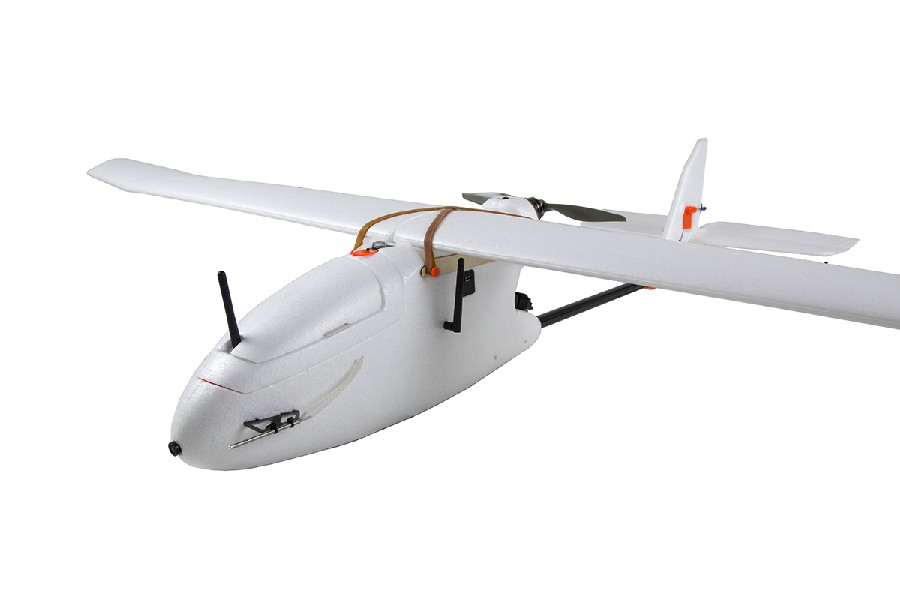
\includegraphics[width=6.5cm,trim=0 0 0 0,clip] {PaperFigures/fixedwing}}
		\subfigure []{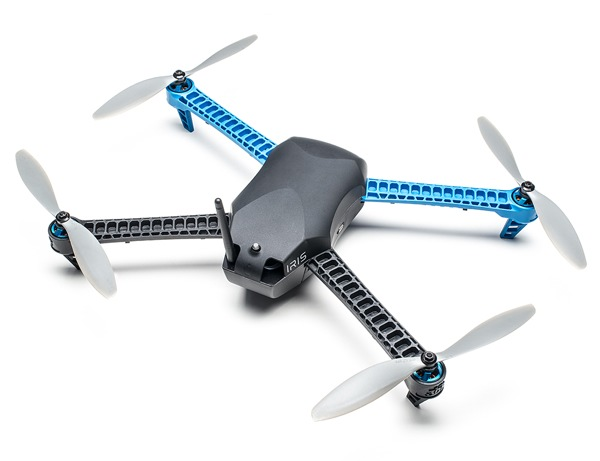
\includegraphics[width=6.5cm,trim=0 0 0 0,clip] {PaperFigures/iris-1}}
		\hspace*{0mm}
	\end{subfigmatrix}
	\caption{Fixed Wing UAV (a) and Multirotor UAV (b)}
	\label{fig:fixedMultirotor}
\end{figure}

UAVs can be programmed to fly autonomously without the direct input of a pilot. When flying autonomously, the vehicle typically accomplishes tasks by following a pre-planned flight path. Flight paths are often generated off-line at dedicated ground station and relayed to the UAV over radio. 

\subsection{Ground Stations}
Ground stations are the software framework used to configure UAV settings, plan missions, and collect mission data. Commercial open source ground stations such as QGround Control \cite{qgc} depend on a human operator's knowledge of the environment to plan an obstacle free path. Takeoff, landing, and emergency return-to-home locations are designated in safe clearings capable of accommodating the vehicle. Other tasks such as area surveying and loitering can be assigned at certain points along the mission path \cite{wilhelm_direct_2017}. An example of a mission path consisting of taking off, surveying, and landing is shown in Figure \ref{fig:groundstationplanning}




\begin{figure}[H]
	\centering
	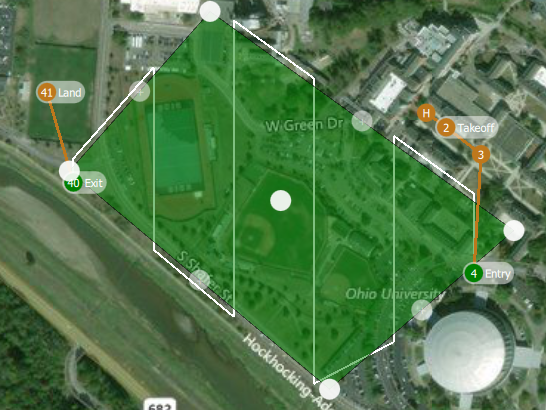
\includegraphics[width=12cm]{PaperFigures/Literature/groundStationPlanning}
	\caption{Ground Station Software Planning a Waypoint Based Mission}
	\label{fig:groundstationplanning}
\end{figure}




\subsection{Autopilot}
Paths are commonly represented as a series of finite waypoints in commercial UAV autopilots such as  the Piccolo \cite{piccolo}, Kestral \cite{kestrel}, and Pixhawk \cite{pix}. The UAV autopilot is responsible for controlling a pre-planned path and maintaining vehicle stability while under the influence of environmental disturbances. Stable flight while path following is accomplished by implementing feed-back control, navigation, and guidance systems \cite{beard_small_2012}. Feed-back refers to the closure of an open-loop control system which allows a reference error to be calculated between the desired state of the UAV, the reference, and the current state of the UAV. Reference error is used to calculate the actuator output required to modify the vehicle's attitude and position while preventing unbounded oscillation. Attitude and position feed-back is provided by the navigation system by sampling on-board sensors such as global position system (GPS) and inertial measurement units (IMUs). Filtering and fusing noisy data from multiple sources is often accomplished through estimation techniques such as the Kalman filter \cite{de_marina_guidance_2017}. The guidance system directs the UAV with a commanded heading towards a desired goal, such as a waypoint or path. A high level overview of the autopilot's systems can be seen in Figure \ref{fig:autopilotloops}. When simulating new guidance or navigation systems it is common to model the plant as a Dubin's vehicle with turn rate constraints for simplicity. UAVs are high order and non-linear systems that can be represented as a Dubin's vehicle \cite{beard_small_2012}.



%\begin{figure}
%	\centering
%	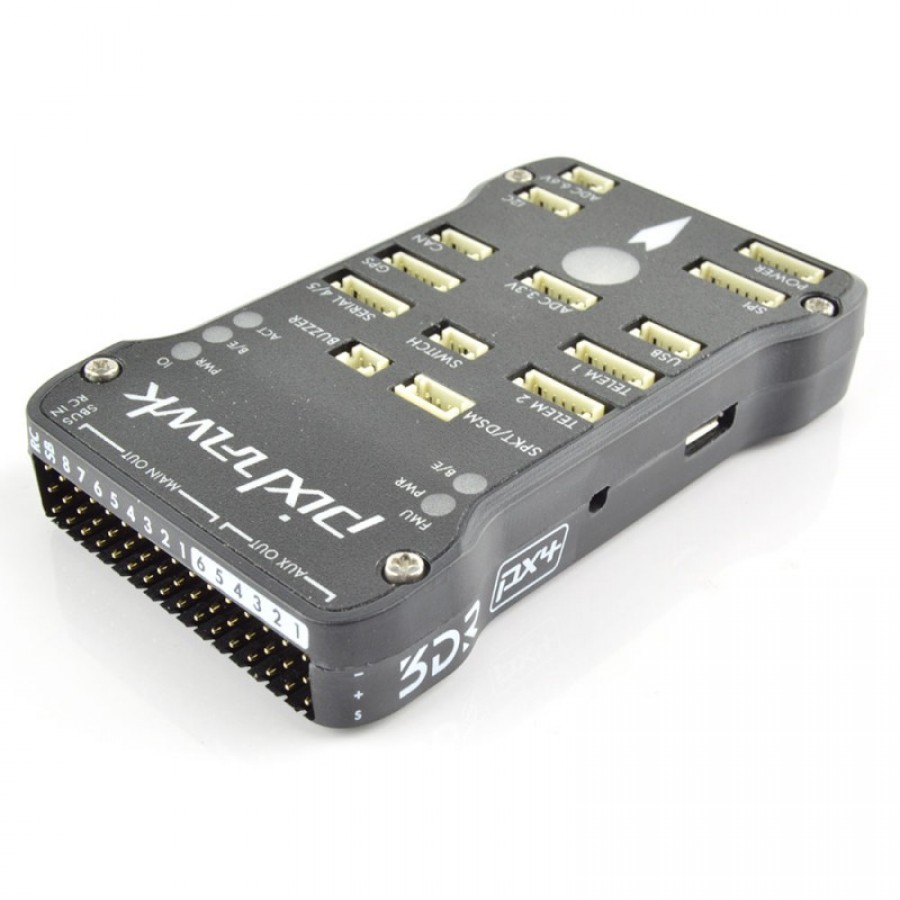
\includegraphics[width=8cm]{PaperFigures/pixhawk}
%	\caption{Pixhawk autopilot}`
%	\label{fig:pixhawk}
%\end{figure}
%
%
%



%\begin{figure}
%	\centering
%	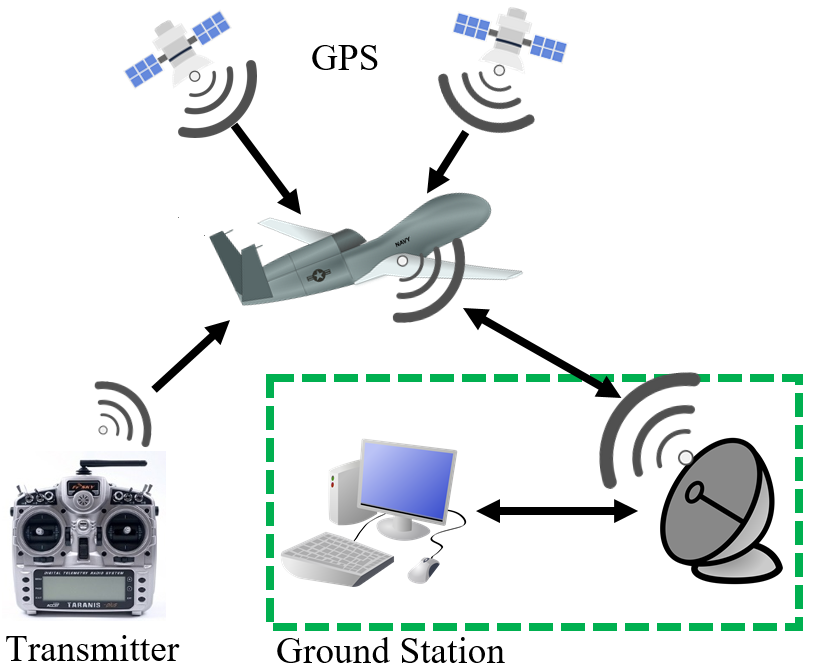
\includegraphics[width=12cm]{PaperFigures/UAS}
%	\caption{Unmanned Aerial System (UAS)}
%	\label{fig:uas}
%\end{figure}

\begin{figure}[H]
	\centering
	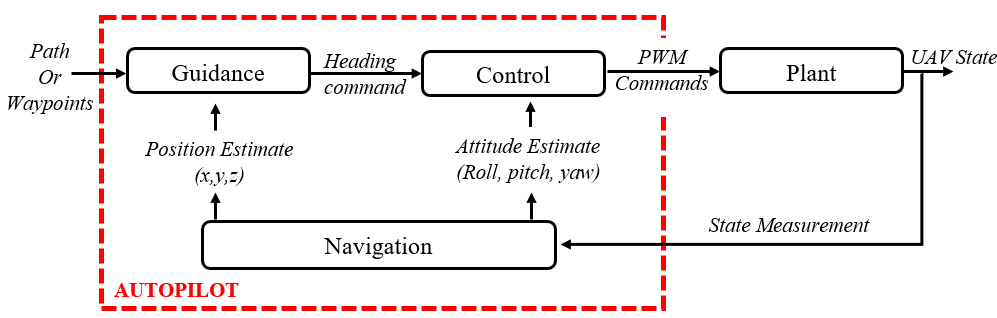
\includegraphics[width=15cm]{PaperFigures/autopilotLoops2}
	\caption{Autopilot's Navigation, Guidance, and Control Architecture}
	\label{fig:autopilotloops}
\end{figure}

\section{Dubins Vehicle Model}
The dynamics of a UAV are often simplified by modeling the UAV as a Dubin's vehicle when simulating guidance systems \cite{frew_cooperative_2007,griffiths_vector_2006,nelson_cooperative_2005,nelson_vector_2006,nelson_vector_2007}. It is assumed that the autopilot's control system is capable of maintaining stability, speed $u$, and altitude, and can turn the vehicle at a maximum fixed turn rate $\dot{\theta}$. The position of the UAV $\overrightarrow{X}$ at time $t$ is calculated from the integral of the velocity vector $\overrightarrow{U}$, Equation \ref{eq:uavPosition}. Heading $\theta$ is an input from a guidance system. Here the turn rate of the UAV is restricted to $20$ degrees per second which is typical for small unmanned aircraft.
\begin{equation}
\label{eq:uavVelocity}
\overrightarrow{U}(t) = u \begin{bmatrix}
cos(\theta(t)) \\
sin(\theta(t))
\end{bmatrix}
\end{equation}


\begin{equation}
\label{eq:uavPosition}
\overrightarrow{X}(t) = \overrightarrow{U}dt + \overrightarrow{X}(t-1)
\end{equation}


\begin{equation}
\label{turnRate}
\dot{\theta} \leq 20 deg/s
\end{equation}


\section{UAV Guidance}
Guidance methods for following a pre-planned path include geometric methods such as waypont \cite{osborne_waypoint_2005} or carrot chasing \cite{manjunath_application_2016} and control techniques such as proportional-integral-derivative (PID) \cite{rhee2010tight}, non-linear guidance laws \cite{park2007performance}, and linear quadratic regulator (LQR) \cite{ratnoo_adaptive_2011}. These methods may not have the ability to avoid new or previously unknown obstacles without the need to generate a new path. Re-planning and relaying a new obstacle free path may be impossible under certain conditions, such as flying beyond radio communication range. It would be beneficial to remove the guidance system's dependence on the path planner to produce a new obstacle free path when new obstacles are encountered. Avoiding obstacles without the need to re-plan has been achieved with potential field and vector field, which represents obstacles as artificial repulsive forces that locally push away from obstacles. 

\subsection{Potential Field}

Potential field is based on the principle of driving a point mass from a high potential state to a globally low potential state using artificial attractive and repulsive forces \cite{khatib_real-time_1986}. An attractive force directs the point mass in the direction of a goal located at a globally minimum potential and obstacles can be represented as repulsive forces that act locally to push the point mass away. An example of a point mass directed by potential field from a high potential to a globally minimum potential while avoiding an obstacle is shown in Figure \ref{fig:pfobstacle}. Potential field is also capable of acting as a path and trajectory planning algorithm \cite{rimon_exact_1992}, possibly eliminating the off-board path planner. 

\begin{figure}[H]
	\centering
	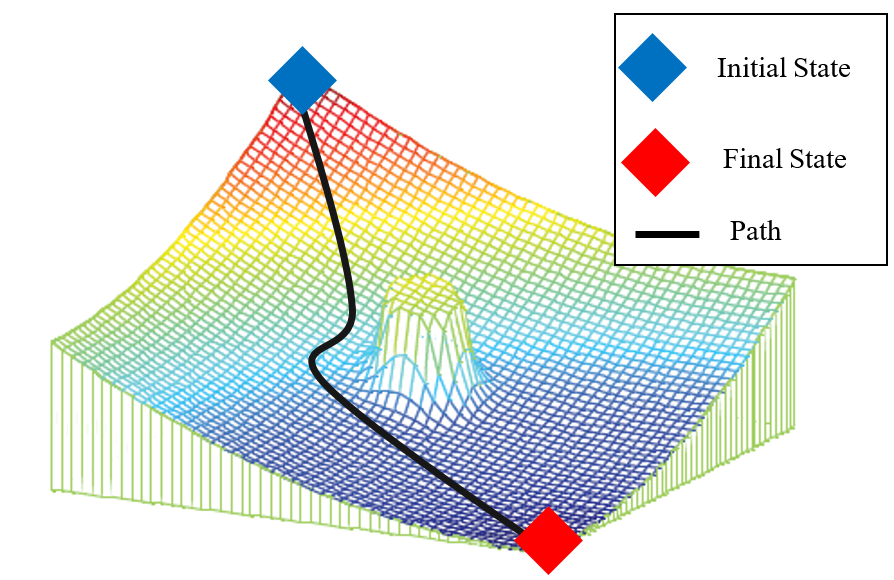
\includegraphics[width=10cm]{PaperFigures/pfObstacle}
	\caption{Single Obstacle Potential Field Gradient \cite{liu_virtual-waypoint_2016}}
	\label{fig:pfobstacle}
\end{figure}


An implementation of potential field on a mobile ground robot equipped with ultrasonic sensors for real-time obstacle detection can be found in \cite{borenstein_real-time_1990,borenstein_vector_1991,koren_potential_1991}. A differential drive robot was guided  with the guidance, $\overrightarrow{R}$, which directed the robot towards a goal and away from nearby obstacles. The robot was attracted towards a goal with constant magnitude force, $\overrightarrow{F_t}$, located at $(x_t,y_t)$ and a distance $d_t$ from the robot. In the immediate area of the robot, an active window recorded integer certainty values inside discrete cells. Cells containing an obstacle provide a repulsive force, $\overrightarrow{F_{i,j}}$, opposite in direction to the line-of-sight from vehicle to cell location $(x_i,y_j)$, where $(i,j$) represents the cell index, $F_{cr}$ is a constant repulsive force, $W$ the vehicle's width, $C_{i,j}$ a cell's certainty, and $d_{i,j}$ the distance to the center of the cell with respect to robots center.

\begin{equation}\label{eq:vffHeading}
\overrightarrow{R} = \overrightarrow{F_r} + \overrightarrow{F_t}
\end{equation} 



\begin{figure}[H]
	\centering
	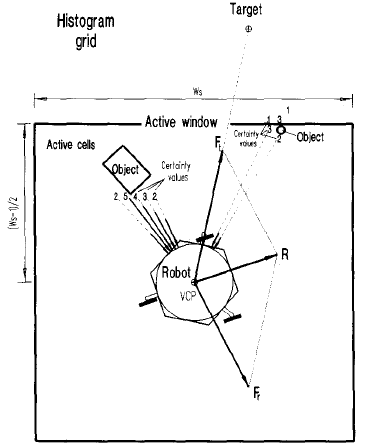
\includegraphics[width=7cm]{PaperFigures/histogram}
	\caption{Virtual Force Field Histogram Guiding a Mobile Robot \cite{borenstein_vector_1991}}
	\label{fig:histogram}
\end{figure}

\begin{equation}\label{eq:vffRepulse}
\overrightarrow{F_{i,j}} = \frac{F_{cr}W^nC_{i,j}}{d^n_{i,j}} \bigg( \frac{x_i-x_0}{d_{i,j}}\hat{x} + \frac{y_i-y_0}{d_{i,j}}\hat{y}\bigg)
\end{equation}

\noindent
The total repulsive force exerted on the robot is determined by summing the active cells, shown in Equation \ref{eq:vffRepulseSum}


\begin{equation}\label{eq:vffRepulseSum}
\overrightarrow{F_r} = \sum_{i,j}\overrightarrow{F_{i,j}}
\end{equation}


\begin{equation}\label{eq:vffGoal}
\overrightarrow{F_t} = F_{ct} \bigg( \frac{x_t-x_0}{d_{t}}\hat{x} + \frac{y_t-y_0}{d_{t}}\hat{y}\bigg)
\end{equation}


Major drawbacks to potential field were identified in \cite{koren_potential_1991} consisting of local minimum and oscillations in corridors. Local minimum are solutions in the potential field that are caused by the close spacing of obstacles which may result in a well that can trap the system into a local stable point prior to reaching the global minimum. A scenario similar to that shown in Figure \ref{fig:pfobstacle} with two more obstacles results in a trap situation where the state settles into a well on the gradient, shown in Figure \ref{fig:pfLocalMin}. Additionally, closely spaced obstacles may also be difficult to pass between, shown in Figure \ref{fig:vff}a. Oscillations can also be experienced near obstacles or in narrow passages at high speeds, shown in Figure \ref{fig:vff}b.



 

\begin{figure}[H]
	\begin{subfigmatrix}{2}% number of columns
		\centering
		\subfigure []{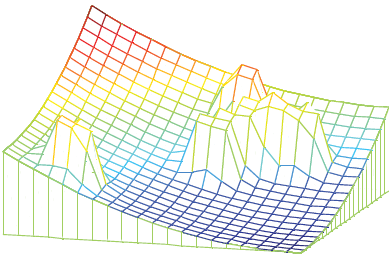
\includegraphics[width=7cm] {PaperFigures/pfObstacleLocalMin}}
		\subfigure []{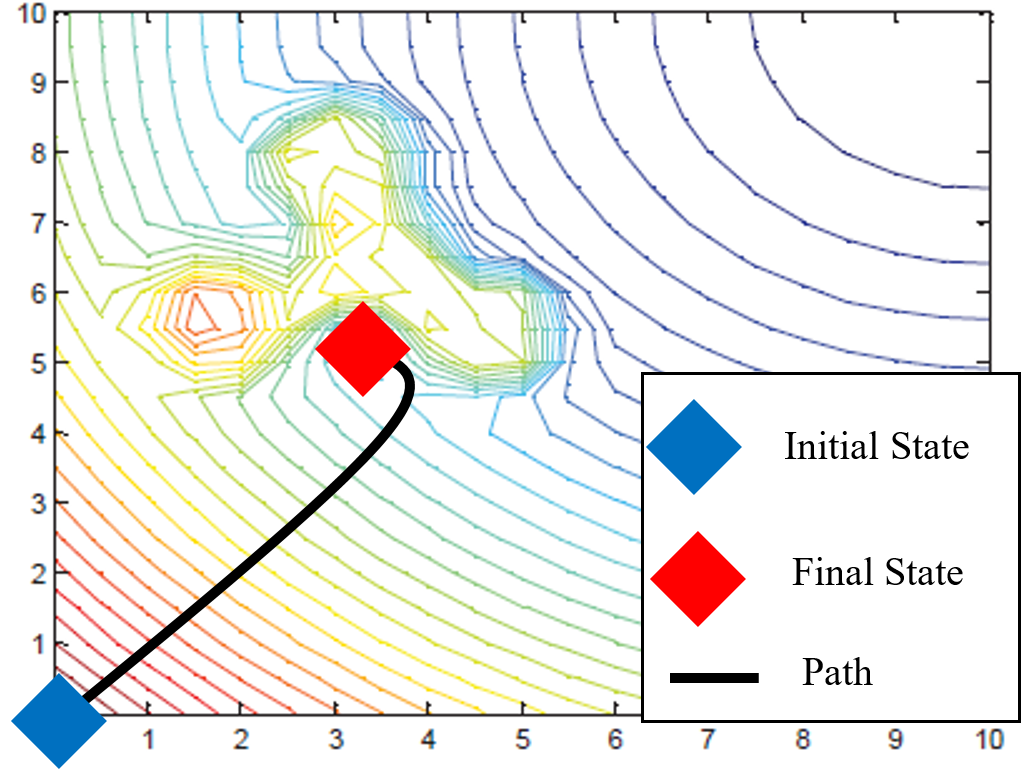
\includegraphics[width=7cm] {PaperFigures/pfObstacleLocalMinTopology}}
	\end{subfigmatrix}
	\caption{Potential Field Local Minimum \cite{liu_virtual-waypoint_2016}}
	\label{fig:pfLocalMin}
\end{figure}

Proposed solutions to local minimum include object clustering and virtual waypoint method \cite{liu_virtual-waypoint_2016}, virtual escaping route \cite{kim_escaping_2009}, and use of navigation functions \cite{goerzen_survey_2010}. Oscillations in potential field were addressed in \cite{lei_tang_novel_2010} and \cite{li_efficient_2012}.

\begin{figure}[H]
	\begin{subfigmatrix}{2}% number of columns
		\centering
		\subfigure []{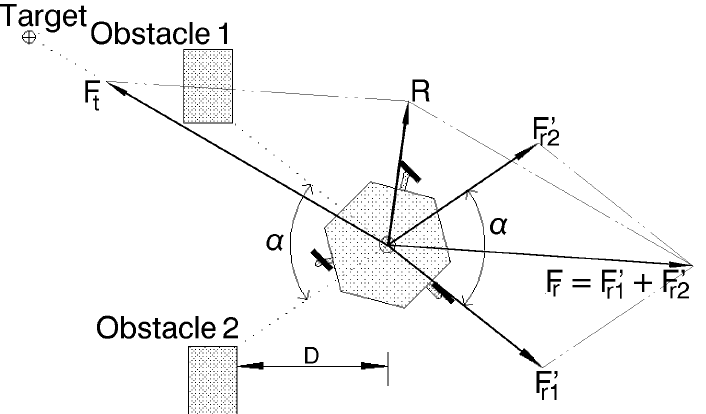
\includegraphics[width=9cm] {PaperFigures/multipleObsVff}}
		\subfigure []{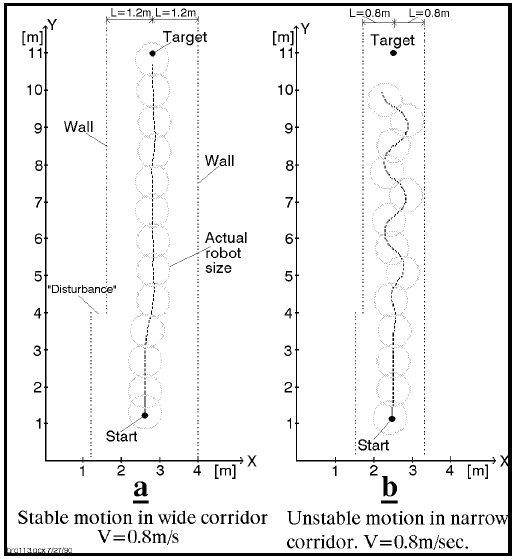
\includegraphics[width=6cm] {PaperFigures/unstableCooridorMotionVff}}
	\end{subfigmatrix}
	\caption{Potential Field Local Minimum \cite{liu_virtual-waypoint_2016}}
	\label{fig:vff}
\end{figure}

Navigation functions \cite{goerzen_survey_2010} and obstacle clustering \cite{liu_virtual-waypoint_2016} have been used to prevent local minimums in potential field. Navigation functions relate kinematic constraints to the gradient potential to produce a bounded and local minimum free solution \cite{rimon_exact_1992}. Clustering closely spaced obstacles into a single and equally repulsive obstacle prevents local minimum from forming, shown in Figure \ref{fig:obstacleclustering}.  

\begin{figure}[H]
	\centering
	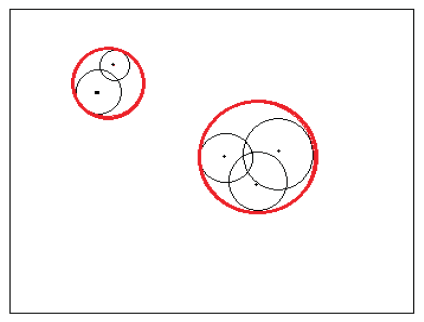
\includegraphics[width=6cm]{PaperFigures/obstacleClustering}
	\caption{Obstacle Clustering to Prevent Local Minimum \cite{liu_virtual-waypoint_2016}}
	\label{fig:obstacleclustering}
\end{figure}


Potential Field's ability to avoid obstacles and combine path planning, trajectory planning, and control into a single system makes it an attractive guidance method for robots seeking a singular point, even with the limitations discussed in \cite{koren_potential_1991}. Unlike the mobile ground robots in \cite{borenstein_real-time_1990}, fixed wing UAVs must maintain a minimum forward velocity, have limited turning radius, and cannot converge to a single point. Vehicles with velocity and turn rate constraints may not return to a pre-planned path once the obstacle has been avoided, shown in Figure \ref{fig:vffSimulated}. Methods that direct a UAV to a path instead of a discrete point has been achieved with Lyapunov and gradient vector fields. 


\begin{figure}[H]
	\centering
	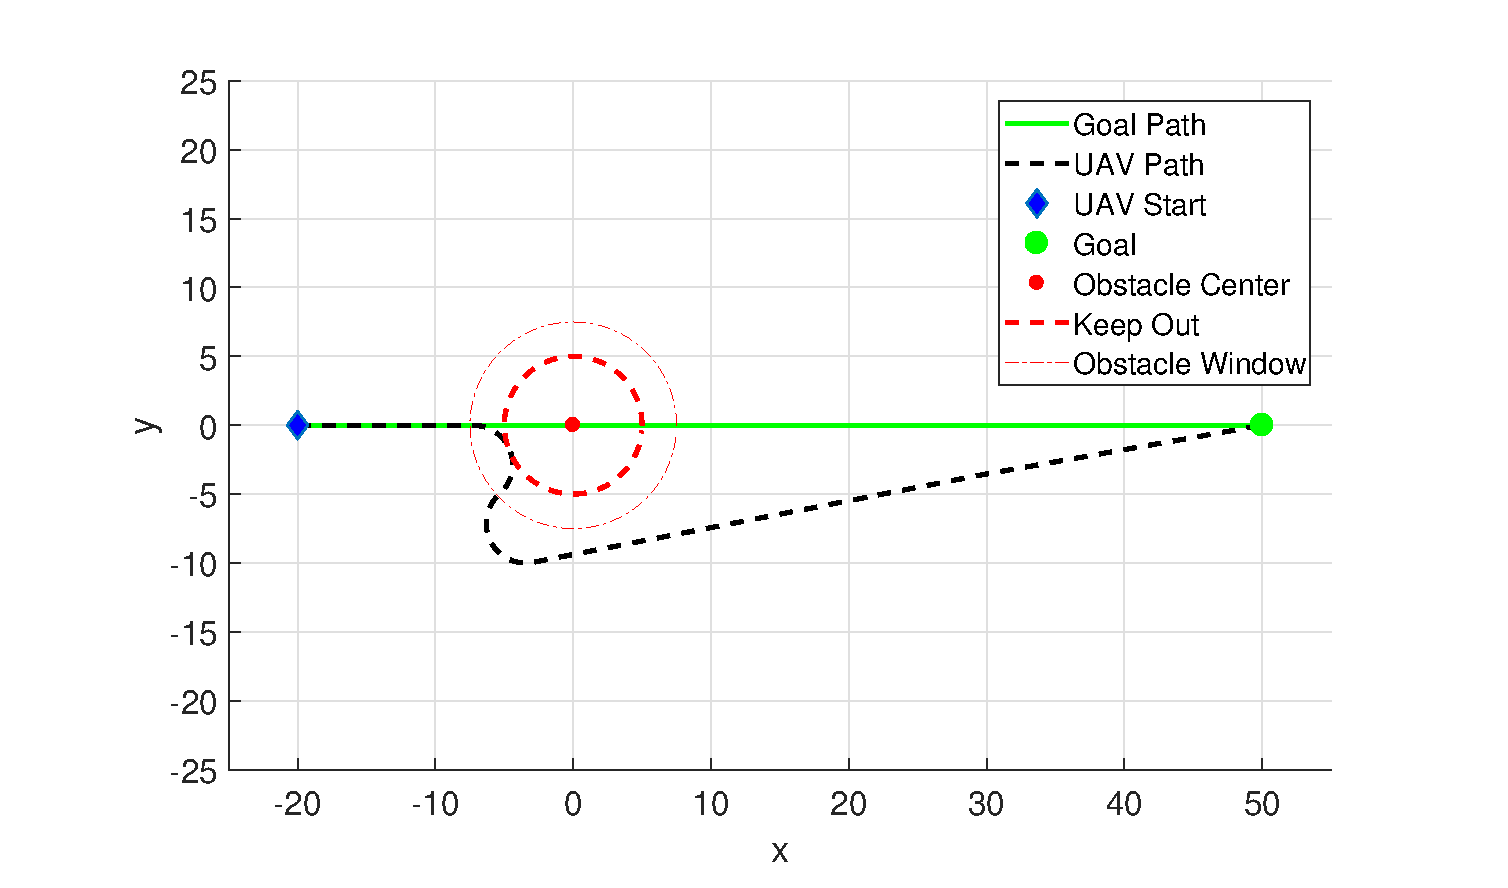
\includegraphics[width=15cm]{PaperFigures/Literature/vffSimulated}
	\caption{UAV Avoiding Obstacle with VFF Guidance}
	\label{fig:vffSimulated}
\end{figure}



\subsection{Lyapunov Vector Fields}
Lyapunov vector fields for converging and following straight and circular paths were described in \cite{nelson_cooperative_2005}. For converging and following a straight path, a guidance vector $\chi^{d}$ is determined in Equation \ref{eq:lyapunovStraight}, where $\chi^{\infty}$ is the course approach angle, $y$ is the lateral distance to the path, and $\bar{k}$ is a positive constant that determines the rate of transition between convergence and following. An example of a Lyapunov vector field converging and following a straight line is shown in Figure \ref{fig:vfPathPrimitives}a.


\begin{equation}\label{eq:lyapunovStraight}
\chi^d(y) = -\chi^{\infty}\frac{2}{\pi}\tan^{-1}(\bar{k}y)
\end{equation}



For converging and following a circular path, a guidance vector $\chi^{d}$ is determined in Equation \ref{eq:lyapunovCirc}, where $\psi$ is the UAVs angular position with respect to the circle, $r$ is the paths radius, $d$ is the distance from the circles center, and $\bar{k}$ is a positive constant that determines the transition behavior. An example of a Lyapunov vector field for converging and following a circular path is shown in Figure \ref{fig:vfPathPrimitives}b.

\begin{equation}\label{eq:lyapunovCirc}
\chi^d(d) = \psi-\frac{\pi}{2}-\tan^{-1} \bigg(\bar{k} \frac{d-r}{r} \bigg)
\end{equation}


\begin{figure}
	\centering
	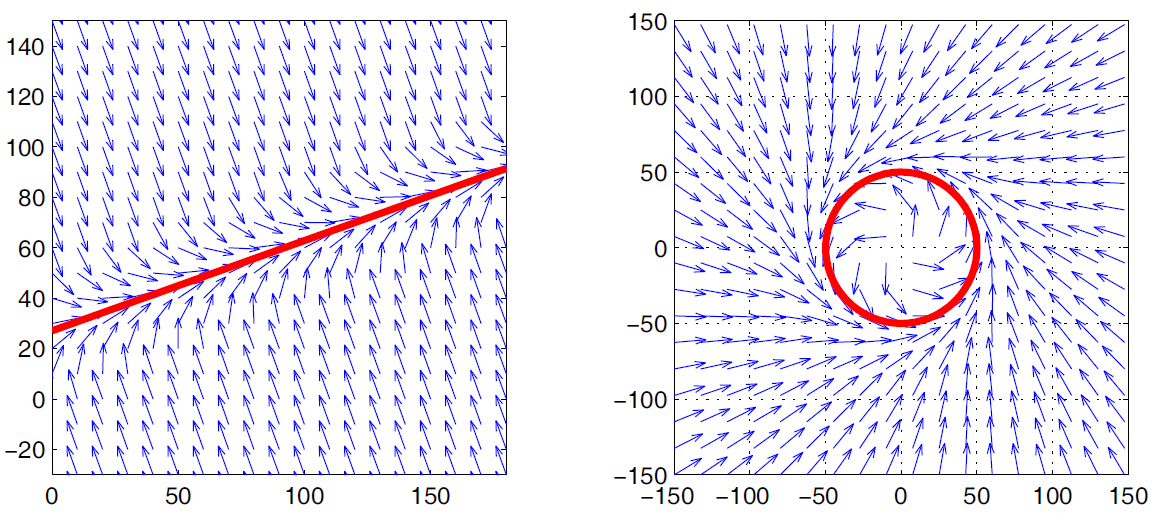
\includegraphics[width=13cm]{PaperFigures/nelsonLyapunov}
	\caption{Lyapunov Vector Field for Straight Line and Circular Primitives \cite{nelson_cooperative_2005}}
	\label{fig:vfPathPrimitives}
\end{figure}




Straight and circular path vector fields can be selectively activated throughout flight to form more complex paths, shown in \cite{nelson_cooperative_2005,nelson_vector_2006,nelson_vector_2007,jung_unmanned_2016} and Figure \ref{fig:urbanfollowingnelson}. Selectively activating, or stitching together, vector fields to produce more complex paths was the preferred method in \cite{nelson_cooperative_2005} since summing together multiple fields has the possibility to produce dead zones, sinks, and singularities.
 

\begin{figure}[H]
	\centering
	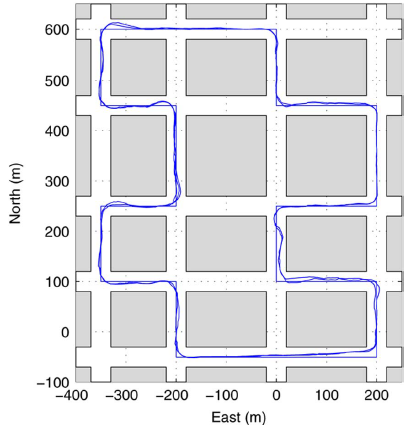
\includegraphics[width=7cm]{PaperFigures/urbanFollowingNelson}
	\caption{Straight Path Following in Urban Environment \cite{nelson_cooperative_2005} using Lyapunov Vector Field}
	\label{fig:urbanfollowingnelson}
\end{figure}

Lyapunov Vector field construction for curved paths was presented in \cite{griffiths_vector_2006} and is shown in Figure \ref{fig:griffiths}. Constructing a Vector Field for an arbitrary curve may allow for more complex paths and could eliminate the need for switching between primitives. 

\begin{figure}[H]
	\centering
	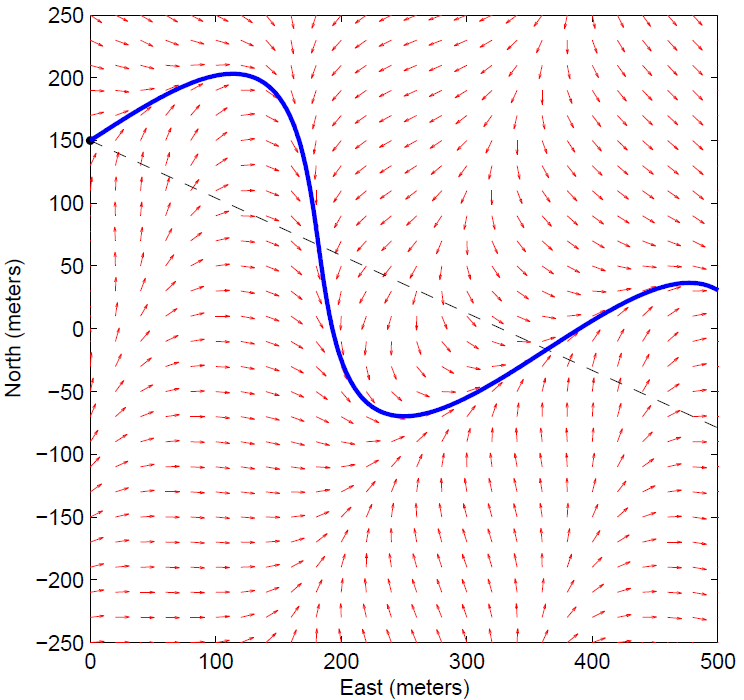
\includegraphics[width=7cm]{PaperFigures/griffiths}
	\caption{Lyapunov Vector Field Approach Curved Path \cite{griffiths_vector_2006}}
	\label{fig:griffiths}
\end{figure}


Primitive circular vector fields were modified in \cite{frew_lyapunov_nodate,frew_cooperative_2007} via non-linear coordinate transformations to produce elliptical \ref{fig:lyapunovFrew}a, or racetrack \ref{fig:lyapunovFrew}b, fields. Transforming the circular field as a function of a Kalman filter's covariance matrix when sensing an uncertain target was investigated in \cite{frew_cooperative_2007}. 

\begin{figure}[h]
	\begin{subfigmatrix}{2}% number of columns
		\centering
		\subfigure []{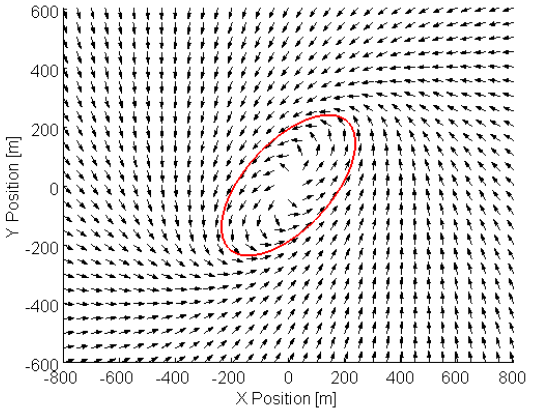
\includegraphics[width=8cm] {PaperFigures/lyapunovFrewUncertain}}
		\subfigure []{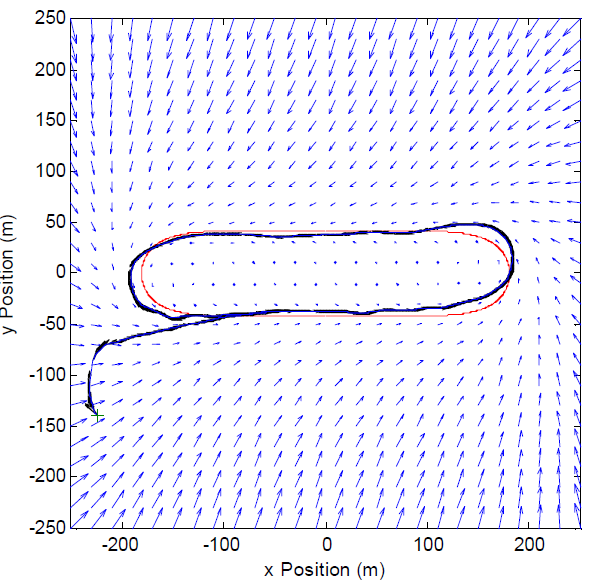
\includegraphics[width=6.25cm] {PaperFigures/lyapunovFrew}}
		%		\hspace*{1cm}
	\end{subfigmatrix}
	\caption{Elliptical VF Produced by Non-linear Coordinate Transformations a)\cite{frew_cooperative_2007} and b) \cite{frew_lyapunov_nodate}}
	\label{fig:lyapunovFrew}
\end{figure}

Target tracking Tangent Plus Lyapunov Vector Field (TPLVF) was introduced in \cite{chen_tracking_2009} that produced shorter paths compared to Lyapunov alone. Outside of the standoff circle, tangent vectors provided the shortest distance to a standoff circle. Inside the standoff circle, no tangent lines exist and Lyapunov was used in its place. The two paths taken for Lyapunov and tangent vector fields outside the standoff circle are shown in Figure \ref{fig:lyapunovChen}. TPLVF was later used for path planning to avoid obstacles in \cite{chen_uav_2013} while \cite{liang_tangent_2017} constructed a tangent vector field for curved paths.

\begin{figure}
	\centering
	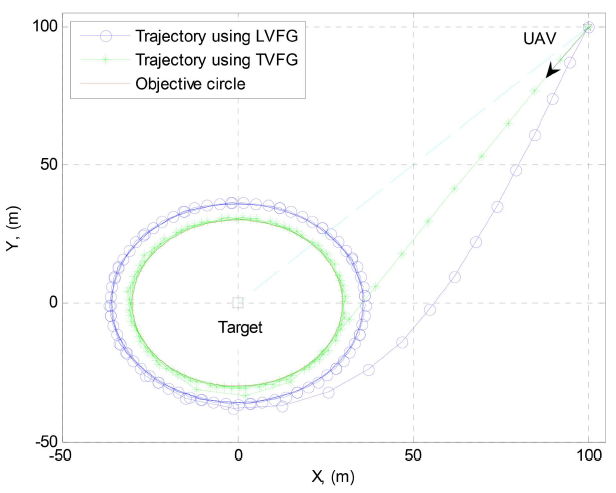
\includegraphics[width=10cm]{PaperFigures/lyapunovChen}
	\caption{Tangent Plus Lyapunov Vector Fields for Shortest Path Target Tracking \cite{chen_uav_2013}}
	\label{fig:lyapunovChen}
\end{figure}


\subsection{Path Planning Vector Fields}
Another use of vector fields is a high level specification for heuristic path planning algorithms \cite{pereira_framework_2016}. An optimal Rapid Random Trees (RRT*) algorithm used a vector field as a guide to explore the configuration space of the UAV for an obstacle free path. Branches extend from the root, or initial location of the UAV, randomly throughout the map with a finite deviation from the initial vector field. When a branch encounters an obstacle it is trimmed and no longer explored. The path of minimum cost, or least distance, is selected for the UAV to use as a reference path. An example of the algorithm is shown in Figure \ref{fig:rrtvf}.

\begin{figure}[H]
	\centering
	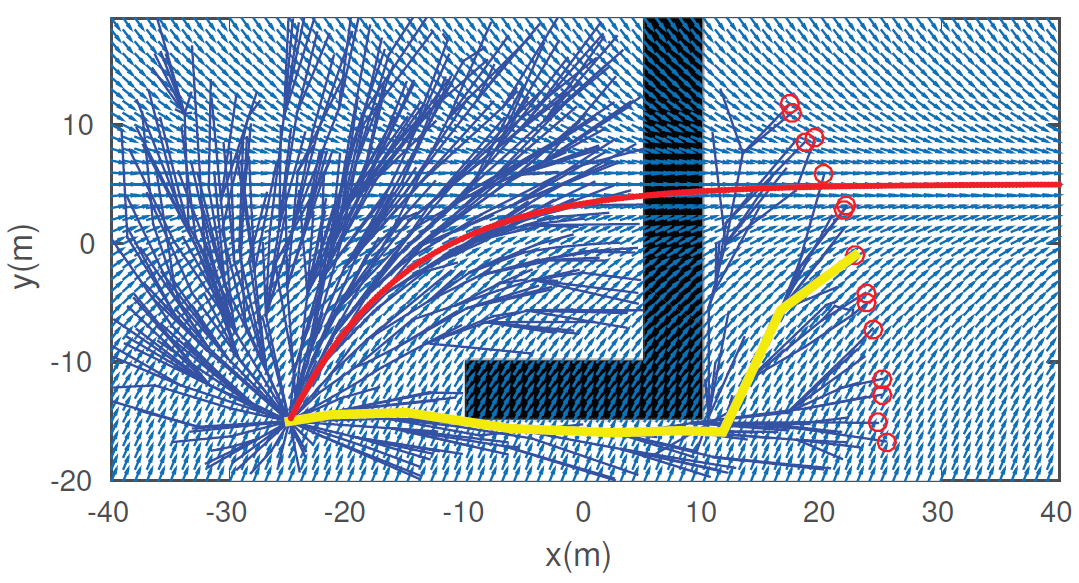
\includegraphics[width=12cm]{PaperFigures/rrtVF}
	\caption{RRT* Path Planner with a VF Used as a Task Specification \cite{pereira_framework_2016}}
	\label{fig:rrtvf}
\end{figure}


A VF was constructed inside a configuration space with edges defined by Delauny triangulation (DT) in \cite{pimenta_fully_2007}.  A simulation of a robot traversing a vector field inside a set of DTs can be seen in Figure \ref{fig:cdtVF}. Vector fields designed to stay inside a region of DTs may be used with optimal path planning algorithms for navigating urban environments \cite{md_simplex_2017}.


\begin{figure}
	\centering
	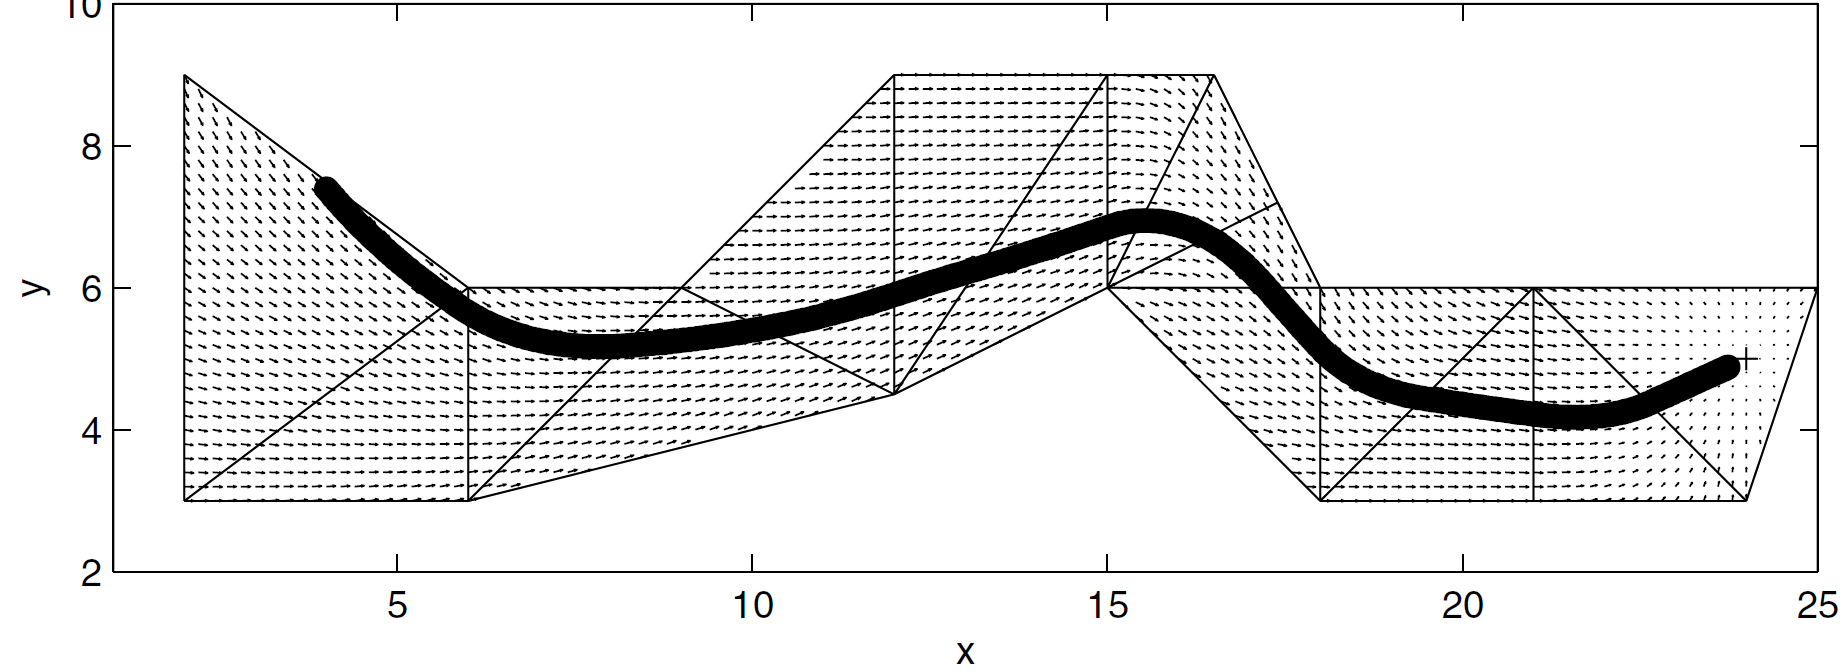
\includegraphics[width=15cm]{PaperFigures/cdtVF}
	\caption{Vector Field Within a Set of Delaunay Triangles \cite{pimenta_fully_2007}}
	\label{fig:cdtVF}
\end{figure}

So far all of the vector field methods discussed have avoided obstacles by planning paths around them. Paths are typically calculated at the ground station and if communication is lost a new path may not be relayed to a UAV encountering a new obstacle. A possible solution is using vector fields to provide a repulsive force such as that seen in \cite{panagou_motion_2014,zhou_vector_2014,wilhelm_2019}. 

\subsection{Gradient Vector Field}
The Gradient Vector Field (GVF) method produces a similar field to LVF, however has several advantages. GVF produces an \textit{n}-dimensional vector field that converges and circulates to both static and time varying paths \cite{goncalves_artificial_2009}. Additionally, convergence, circulation, and time-varying terms that make up the GVF are decoupled from each other allowing for easy weighting of the total field \cite{goncalves_circulation_2010}. GVFs converge and circulate at the intersection, or level set, of $n-1$ dimensional implicit surfaces ($\alpha_i:\mathbb{R}^n\rightarrow\mathbb{R} | i=1,...,n-1$). The integral lines of the field are guaranteed to converge and circulate the level set when two conditions are met: $1)$ the implicit surface functions are positive definite and $2)$ have bounded derivatives. Consider the space with dimensions in set \textbf{q}:



\begin{equation}
\mathbf{q} = \begin{bmatrix} x_1, x_2, ..., x_{n}\end{bmatrix}
\end{equation}

\noindent
The total vector field $\overrightarrow{V}$ is calculated by:
\begin{equation}\label{eq:GVF}
\overrightarrow{V} = G \nabla V + H \wedge_{i=1}^{n-1}\nabla_q\alpha_i  - LM(\alpha)^{-1} a(\alpha)
\end{equation}

\noindent
or in component form:

\begin{equation}\label{simpleGVF}
\overrightarrow{V} = \overrightarrow{V}_{conv} + \overrightarrow{V}_{circ} + \overrightarrow{V}_{tv} 
\end{equation}	

\noindent
where $\overrightarrow{V}_{conv}$ produces vectors that converge to the path, $\overrightarrow{V}_{circ}$ produces vectors that circulate the path, and $\overrightarrow{V}_{tv}$ is a feed-forward term that produces vectors accounting for a time varying path. The scalars $G$, $H$, and $L$ weight convergence, circulation, and time varying components respectively. 

\noindent
Convergence is calculated by:

\begin{equation}
% Total field with Conv, Circ, and Time
\overrightarrow{V}_{conv} = G \nabla V  
\label{convOnly}
\end{equation}

\noindent
where scalar $G$ is multiplied by the gradient of the definite potential function $V$ used in \cite{goncalves_circulation_2010}:

\begin{equation}
\label{potentialV}
V = -\sqrt{{\alpha_1}^2 + {\alpha_2}^2}
\end{equation}


\noindent
Circulation is calculated by taking the wedge product of the gradient:

\begin{equation}
% Total field with Conv, Circ, and Time
\overrightarrow{V}_{circ} =  \wedge_{i=1}^{n-1}\nabla\alpha_i 
\label{circOnly}
\end{equation}

\noindent
In the case of $(n=3)$ dimensions the wedge product simplifies as the cross product:

\begin{equation}
% Total field with Conv, Circ, and Time
\overrightarrow{V}_{circ} =  \nabla\alpha_1 \times \nabla\alpha_2 
\label{circOnlySimp}
\end{equation}

\noindent
The feed-forward time-varying component is calculated by:
\begin{equation}
\label{tv}
\overrightarrow{V}_{tv} = M^{-1}a
\end{equation}

\noindent
where,

\begin{equation}
\label{mMatrix}
M =\begin{bmatrix}
\nabla\alpha_1^T \\
\nabla\alpha_2^T \\
(\nabla\alpha_1 \times \nabla\alpha_2)^T
\end{bmatrix}
\end{equation}

\begin{equation}
\label{aVector}
a =\begin{bmatrix}
\frac{\partial \alpha_1}{\partial t} \quad   \frac{\partial \alpha_2}{\partial t} \quad   0
\end{bmatrix}^T
\end{equation}


In \cite{goncalves_artificial_2009,goncalves_circulation_2010,goncalves_vector_2010} GVFs were constructed to control the velocity $\dot{q}$ of a holonomic robot by $\dot{q}=h$. Constant speed  $u$ was controlled by calculating the weighting scalars $G$, $H$, and $L$ that maintained the condition $||\dot{q}|| = u$. Other studies normalized the vector $\overrightarrow{V}$ and used it as a heading guidance while assuming velocity is held constant by the autopilot \cite{gerlach_autonomous_2014,wilhelm_2019}. Assuming velocity is controlled by a separate system frees up the vector field scalars to modify field behavior for other applications, such as specifying circulation direction, transition from convergence to circulation, and repulsion. 
 
 
 The standoff tracking and avoidance scenario presented in \cite{wilhelm_2019} used GVF as a heading guidance and negative GVF convergence weights to produce repulsive fields. A fixed UAV was tasked with loitering around a slow moving ground target while avoiding obstacles. A circular attractive time-varying vector field $\overrightarrow{V}_{p}$ was attached to a moving ground target and summed with repulsive obstacle vector fields $\overrightarrow{V}_{o}$ centered at the obstacles to provide the guidance $\overrightarrow{V}$ in Equation \ref{summedAttRepulsive}. 
 
 
 \begin{equation}
 \overrightarrow{V} = \overrightarrow{V}_{p}+P\overrightarrow{V}_{o}
 \label{summedAttRepulsive}
 \end{equation}
 
 \noindent
 The strength of repulsive obstacle fields were weighted by the hyperbolic tangent decay function $P(d)$ bounded between $[0,1]$ in Equation \ref{repulsiveDecay}, where $d$ is the range to the obstacle's center and $R$ is the radius of at which the function $P$ is near zero. 
 
 the decay, shown in Figure \ref{fig:tanhLit}
 
 \begin{equation}
 P = -R\frac{tanh(2\pi d-\pi)-2}{2}
 \label{repulsiveDecay}
 \end{equation}

\begin{figure}[H]
	\centering
	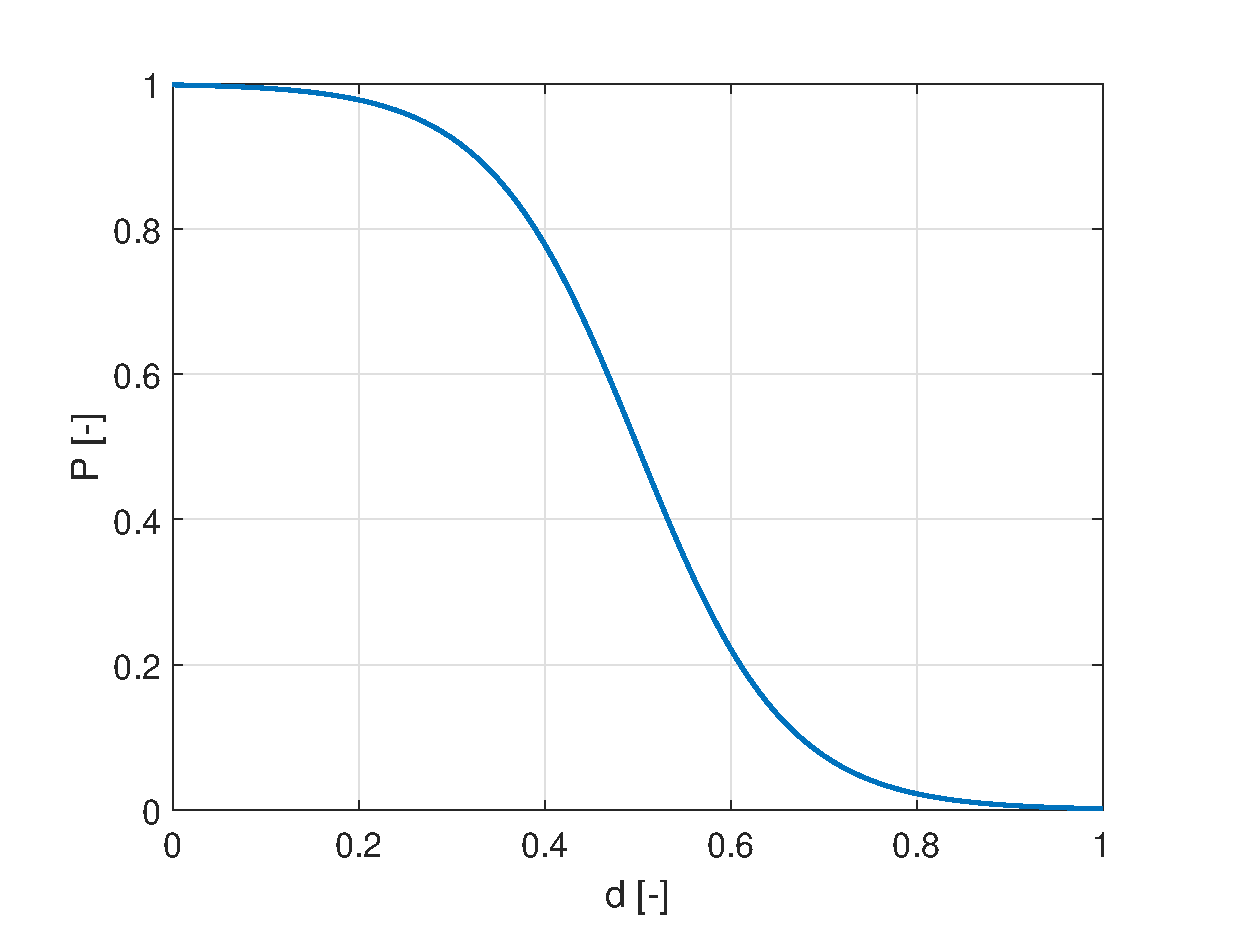
\includegraphics[width=12cm]{PaperFigures/Literature/tanh}
	\caption{Tangent Hyperbolic Function for Obstacle Decay in \cite{wilhelm_2019}}
	\label{fig:tanhLit}
\end{figure}

 
 \noindent
 The performance of LVF [21] and GVF \cite{goncalves_artificial_2009,goncalves_circulation_2010,goncalves_vector_2010} were compared for their cross track error with respect to the loiter circle in \cite{wilhelm_2019}. GVF was shown to have less cross track error compared to LVF due to the compensation for a time-varying vector field attached to the moving target. Avoidance was achieved without the need to re-plan mission paths. Additionally, the GVF avoidance guidance is an algebraic guidance that consists of summing an attractive path with obstacle fields that direct a UAV along the desired route while avoiding obstacles. \\

Summing attractive and repulsive vector fields may result in null guidance where the fields cancel, providing no guidance. The presence of singularities were mentioned briefly in \cite{nelson_cooperative_2005} and observed in \cite{panagou_motion_2014}. For fixed wing UAVs the lack of guidance may prevent the UAV from avoiding an obstacle, while multi-rotor UAVs may end up in a trap situation where they are guided to a singular point. Singularities may be present at any location where a goal field and obstacle field are of equal strength. Further, no optimization to determine what the decay radius or circulation of an avoidance field should be for avoiding an obstacle with the least distance deviation from a planned path. Detecting singularities and modifying the GVF for an improved obstacle avoidance is the contribution of this research.



\section{Literature Review Summary}
UAVs are versatile tools that can be used for remote data collection without putting a pilot in harms way. Tasks are typically accomplished by following a series of waypoints that lie along an obstacle free and flyable pre-planned path. When unplanned or previously unknown obstacles are discovered along the UAVs planned path, a new obstacle free and flyable path may have to be generated which could be impossible if the ground station is beyond communications range. Methods such as potential field and vector field have been used to avoid obstacles without re-planning mission waypoints through the use of artificial attractive and repulsive forces. Potential field is not ideal for fixed wing UAVs since it converges to a singular point whereas LVFs and GVFs can converge and follow paths. GVFs allows for easy weighting of individual convergence and circulation terms making it convenient to modify field behavior without re-solving the Lyapunov equations. A summary of each guidance method discussed is shown in Table \ref{table:compareMeth} below.


\setlength{\tabcolsep}{10pt} % Default value: 6pt
\renewcommand{\arraystretch}{0.5} % Default value: 1
\begin{table}[]
	\caption{Comparison of UAV Guidance Methods}
	\label{table:compareMeth}
	\begin{tabular}{|C{2.5cm}|C{2.5cm}|C{2.5cm}|C{2.5cm}|C{2.5cm}|}	
		\hline
		Guidance Method & Avoids without re-plan    & Returns to path   & De-coupled convergence and circulation vectors       & Time-varying              \\ \hline
		Waypoint        &                           & \Checkmark & N/A                       & N/A                       \\ \hline
		VFF             & \Checkmark &                           &                           &                           \\ \hline
		LVF             & \Checkmark & \Checkmark &                           &                           \\ \hline
		GVF             & \Checkmark & \Checkmark & \Checkmark & \Checkmark \\ \hline
	\end{tabular}
\end{table}


 Summing paths and negating GVF convergence weight can be used for obstacle avoidance, however have so far been used only as high level specification of guidance behavior. Determining repulsive field weights and decay radius has not been optimized for obstacle avoidance. Additionally, characterization of vector field singularities in a summed field has yet to be addressed in literature due to most methods avoiding summation entirely. The contribution of this research is to characterize GVF singularities and provide an optimized decay radius and circulation weight for repulsive fields that minimize path deviation. 

\chapter{Methodology}


\section{Introduction to Methodology}
Circular obstacle avoidance guidance without the need to re-plan a mission path was achieved by summing together a path following and obstacle avoidance vector field with optimized decay and circulation weights. Singularities in summed vector fields were defined and a method for numerically locating their position is presented in Phase I and demonstation of how adding circulation to repulsive GVFs may remove singularities from the UAVs path. Phase II investigated a method for selecting the combination of repulsive GVF decay radius and circulation weights that minimize a path deviation cost function. The optimized GVF guidance was implemented on an indoor multirotor UAV operating under fixed wing constraints in Phase III.


\section{Phase I: Gradient Vector Field Singularity Detection}
 \textbf{The objective of Phase I was to characterize and present a method of locating singularities in a summed gradient vector field.} Phase I presents guidance equations for calculating GVFs that converge and follow a line path using the GVF method in literature \cite{goncalves_artificial_2009,goncalves_circulation_2010,goncalves_vector_2010}. Repulsive GVF for avoiding circular obstacles along the path is achieved by modifying a circular GVF's decay radius, convergence, and circulation weights. Summing the attractive and repulsive GVFs results in guidance that directs the UAV along the planned path while pushing away from the obstacle. Regions in the summed guidance where the path following and obstacle guidance directly oppose each other can result in vectors of zero length, called singularities. A method for identifying the location of singularities is presented along with a method for mitigating them. 
 

\subsection{Path Following Vector Field Guidance}
Two vector fields were constructed consisting of a path following and repulsive obstacle field. Guidance for converging and following a time-invariant path using GVF guidance is achieved by summing together convergence $\overrightarrow{V}_{conv}$ and circulation $\overrightarrow{V}_{circ}$ terms that are multiplied by scalars $G$ and $H$ respectively, shown in Equation \ref{simpleGVF}. The potential function $V$ in Equation \ref{potentialV} decreases asymptotically to null when approaching the target path and therefore the convergence vector begins to decrease as well \cite{goncalves_artificial_2009}. As the potential function decreases, the circulation term begins to dominate the total guidance, promoting path following. The distance from the target path at which the field begins to transition to circulation depends on the scalar weights $G$ and $H$ respectively. The total vector $\overrightarrow{V}_p$ represents the non-normalized attractive path following vector field comprised of both convergence and circulation terms. The shape of the target path that the vectors converge and follow depend on the specification of the implicit 3-dimensional surface functions $\alpha_1$ and $\alpha_2$. Intersecting two planes can be used to generate a GVF that converges and follows a straight path. The vertical plane, described in Equation \ref{eq:pathFunction}, at angle $\delta$ with respect to the paths $y-axis$, is intersected with a horizontal plane at constant altitude $z$, Equation \ref{eq:pathFunctionZ}.



\begin{equation}
\label{eq:pathFunction}
\alpha_1 = cos(\delta)x + sin(\delta)y
\end{equation}

\begin{equation}
\label{eq:pathFunctionZ}
\alpha_2 = z
\end{equation}



\noindent
The gradient of the potential function, $\nabla V$, for calculating the path following convergence term is shown in Equation \ref{eq:potentialFunctionGrad}.

\begin{equation}
\label{eq:potentialFunctionGrad}
\nabla V = \frac{-1}{2(\sqrt{\cos^2(\delta) x^2+2\cos(\delta)\sin(\delta) xy +\sin^2 (\delta) y^2})} \begin{bmatrix}
2x\cos^2(\delta) + 2\cos(\delta)\sin(\delta) y \\
2y\sin^2(\delta) + 2\cos(\delta)\sin(\delta) x \\
2z
\end{bmatrix}
\end{equation}

\noindent
Circulation is calculated by the cross product of the surface function gradients, which evaluates to that shown in Equation \ref{eq:circStraightPart2}.


\begin{equation}
\label{eq:circStraightPart2}
\overrightarrow{V}_{circ} = \begin{bmatrix}
cos(\delta) \\
sin(\delta) \\
0
\end{bmatrix}
\end{equation}

The vector field $\overrightarrow{V}_p$ described will converge and circulate a straight path at the intersection of surfaces $\alpha_1$ and $\alpha_2$, depicted in Figure \ref{fig:planeIntersection}.

\begin{figure}[H]
	\centering
	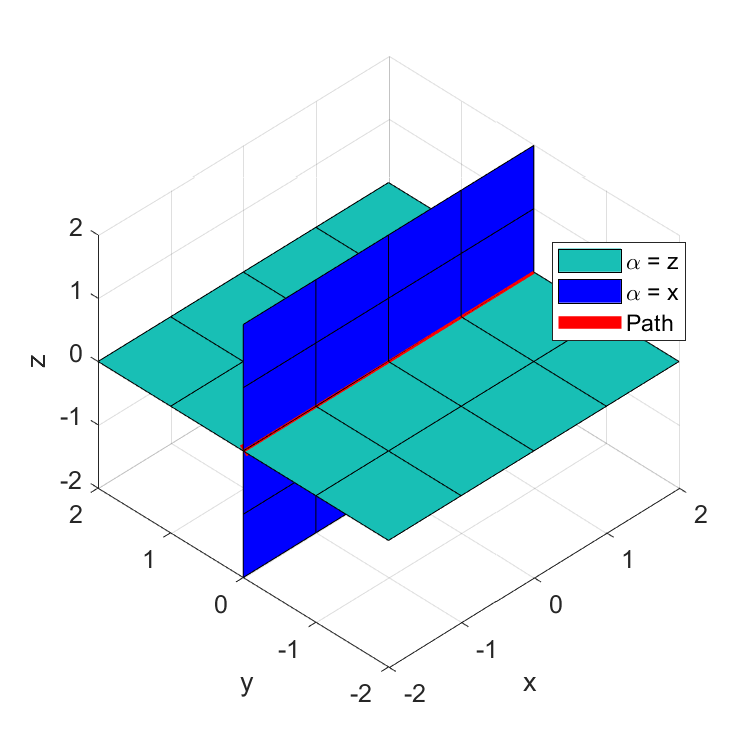
\includegraphics[width=8cm]{Figures/planeIntersection}
	\caption{Intersection of Planes Defined by Implicit Surface Functions}
	\label{fig:planeIntersection}
\end{figure}

Prior to using the path following guidance $\overrightarrow{V}_p$, it is normalized, denoted as $\overrightarrow{V}_{||P||}$, to have a magnitude $||\overrightarrow{V}_p|| = 1$. The reason for normalizing the summed path following vector field is threefold. First, the vector is used as a heading controller only, therefore the angle of the vector is the information required by the autopilot. Second, the normalized vectors result in quiver plots with equal density arrows making the field easier to visualize. Lastly, normalizing the path following vector $\overrightarrow{V}_p$ fixes the length of the vector allowing for prediction of singularity location after summing the field, which will be discussed in the next section. Before discussing singularities, the obstacle field is introduced. 


\begin{equation}
% Component vector field with conv and circ
\overrightarrow{V}_{||P||} = \frac{\overrightarrow{V}_p}{||\overrightarrow{V}_p||}
\label{gonAllCompNormalized}
\end{equation}

To produce guidance for following a path and avoiding an obstacle, a repulsive obstacle vector field $\overrightarrow{V}_{||O||}$ is constructed and summed with the normalized path following guidance $\overrightarrow{V}_{||P||}$. The repulsive vector field is multiplied by a decay function $P$ which limits the influence of the obstacle to a finite range and will be discussed after the avoidance field equations are presented. The sum of the two normalized guidances with obstacle field decay is represented by $\overrightarrow{V}_g$ and is shown in Equation \ref{eq:totalGuidance}


\begin{equation}
\label{eq:totalGuidance}
\overrightarrow{V}_g = \overrightarrow{V}_{||P||} + P\overrightarrow{V}_{||O||}
\end{equation}

\noindent
Constructing the obstacle avoidance vector field $\overrightarrow{V}_{||O||}$ will now be discussed.

\subsection{Constructing an Avoidance Vector Field}

A circular avoidance vector field can be constructed in a way similar to that of the path following field in the previous section. What differentiates the obstacle field from the path following field is that the individual convergence $\overrightarrow{V}_{conv}$ and circulation $\overrightarrow{V}_{circ}$ components are normalized prior to summing to result in the obstacle field $\overrightarrow{V}_o$. The benefit of normalizing each field component before multiplying by their respective scalars $G$ and $H$ prior to summing is to produce an obstacle field with uniform behavior as distance from the obstacle increases. Normalizing each component allows both convergence and circulation terms to be present in the obstacle guidance at larger distances. Additionally, negative convergence weights will be used to produce vectors that diverge away from the path. The obstacle vector field is constructed using the normalized component Equation \ref{eq:obstComponents} with obstacle convergence and circulation weights $G_o$ and $H_o$ respectively.


\begin{equation}
% Component vector field with conv and circ
\overrightarrow{V}_{o} = G_o\frac{\overrightarrow{V}_{conv_{obst}}}{||\overrightarrow{V}_{conv_{obst}}||}+H_o\frac{\overrightarrow{V}_{circ_{obst}}}{||\overrightarrow{V}_{circ_{obst}}||}
\label{eq:obstComponents}
\end{equation}



A circular avoidance vector field with radius $r$ centered at $(x_c,y_c)$ is constructed by intersecting a cylinder, Equation \ref{eq:alphaCylinder}, and a plane Equation \ref{eq:pathFunctionZ}. 

\begin{equation}\label{eq:alphaCylinder}
\alpha_3 = (x-x_c)^2 + (y-y_c)^2-r^2
\end{equation}


Convergence is calculated by the gradient of the potential function in Equation \ref{eq:potentialFunctionGrad}, which when simplified evaluates to

\begin{equation}
\nabla V = A\overrightarrow{B}
\label{eq:AB}
\end{equation}

\noindent
where


\begin{equation}
A = \dfrac{-1}{\sqrt{\bar{x}^4+\bar{y}^4+2\bar{x}^2\bar{y}^2-2r^2\bar{x}^2-2r^2\bar{y}^2+r^2+z^2}}
\end{equation}

\begin{equation}
\overrightarrow{B} = \begin{bmatrix} 2\bar{x}^3+2\bar{x}\bar{y}^2-2r^2\bar{x} \\ 2\bar{y}^3+2\bar{x}^2\bar{y}-2r^2\bar{y} \\z \end{bmatrix}
\end{equation}

\noindent
and


\begin{equation}
\bar{x} = x - x_c
\end{equation}
\begin{equation}
\bar{y} = y - y_c
\end{equation}


Evaluating equation \ref{eq:AB} results in a vector field that converges to a circular path. Circulation is calculated from the cross product of each implicit surface function's gradient, which simplifies to



\begin{equation}
\label{eq:vcirc_circle}
\overrightarrow{V}_{circ_{obst}} =  \begin{bmatrix}  2(y-y_c) \\[6pt] -2(x-x_c) \\[6pt] 0\end{bmatrix}
\end{equation}

The guidance $\overrightarrow{V}_o$ described by intersecting a cylinder and a plane can be shown in Figure \ref{fig:cylinderIntersection}. 

\begin{figure}[H]
	\centering
	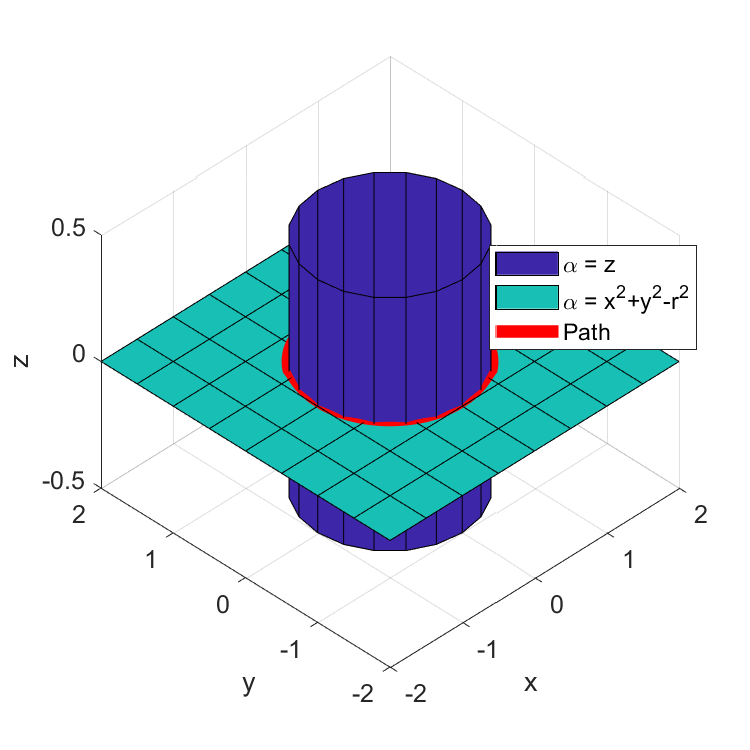
\includegraphics[width=10cm]{Figures/cylinderIntersection}
	\caption{Intersection of a Cylinder and Plane Defined by Implicit Surface Functions}
	\label{fig:cylinderIntersection}
\end{figure}

Obstacle fields should only act locally on the UAV guidance, which is accomplished by applying a decay function for a field of radius $R$. The decay strength $P$ is determined in \ref{eq:decay}, where $d$ is the Euclidean distance, or range, between the UAV and the center of the obstacle, shown in Equation \ref{eq:range}. At a distance $d>R$ the decay strength $P$ is effectively zero, having virtual no influence on the total guidance. At a distance $d\leq R$, the field strength is bounded between $[0,2]$. The selection of the decay function $P$ to be bounded as such is so that the obstacle field $\overrightarrow{V}_o$ eventually overpowers the path field $\overrightarrow{V}_{||P||}$. 


\begin{equation}
\label{eq:decay}
P = -\tanh \bigg( \frac{2\pi d}{R}-\pi\bigg)+1
\end{equation}

\begin{equation}
\label{eq:range}
d = \sqrt{ \bar{x}^2+\bar{y}^2}
\end{equation}


Prior to applying the decay function $P$ the obstacle field $\overrightarrow{V}_o$ is normalized. Forcing the obstacle guidance $\overrightarrow{V}_{||o||}$ to have unity magnitude, bounds the decayed guidance magnitude $P\overrightarrow{V}_{||o||}$ to the interval $[0,2]$ which allows a prediction of singularity location based on the range from obstacle center, $d$.


\begin{equation}
% Component vector field with conv and circ
\overrightarrow{V}_{||o||} = \frac{\overrightarrow{V}_{o}}{||\overrightarrow{V}_{o}||}
\label{eq:obstNormalized}
\end{equation}


\subsection{Summed Guidance and Singularity Definition}
The total summed guidance $\overrightarrow{V}_g$ defined in Equation \ref{eq:totalGuidance} can now be calculated and visualized, Figure \ref{fig:summedFieldsNoNorm}. In general, the GVF guidance is normalized for plotting, however, plotting the non-normalized guidance $\overrightarrow{V}_g$ demonstrates regions where the fields oppose each other and decrease the total fields magnitude. Guidance from summing a strictly repulsive field that is centered on a straight path, regions of both constructive and destructive summation occurs. Note the vectors on the positive x-axis increasing in length as the two fields come together. Conversely, vectors in the negative x-axis show decreasing length and in some areas disappearing entirely.  

\begin{figure}[H]
	\centering
	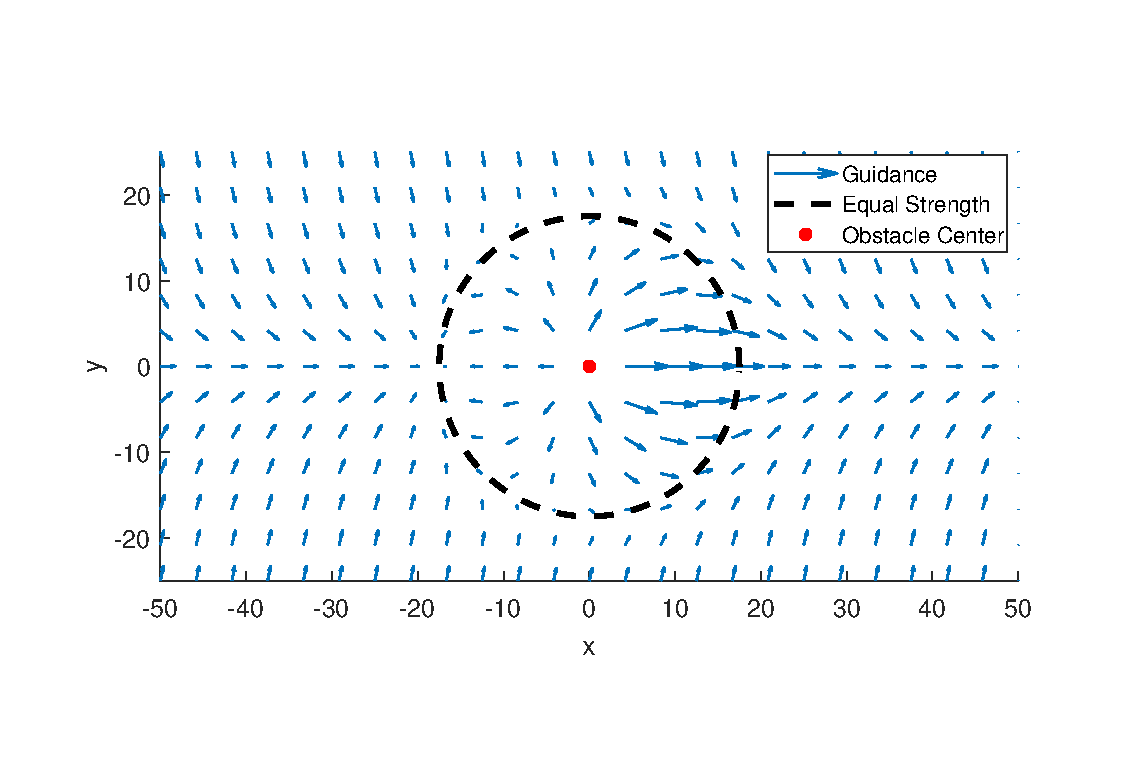
\includegraphics[trim=25 35 25 50,clip,width=14cm]{PaperFigures/Methods/summedFieldsNoNorm}
	\caption{Summed Fields Without Total Normalization $\protect \overrightarrow{V}_g$ with Null Circulation}
	\label{fig:summedFieldsNoNorm}
\end{figure}

Observing the regions around disappearing vectors it is shown that vectors appear to converge to a singular point from all directions, possibly indicating a trap situation. Visualizing the vector magnitudes of the scenario presented above can be accomplished with a summed field heat map, shown in Figure \ref{fig:summedHeatMap}, which shows the regions of decreasing magnitude more clearly. 


\begin{figure}[H]
	\centering
	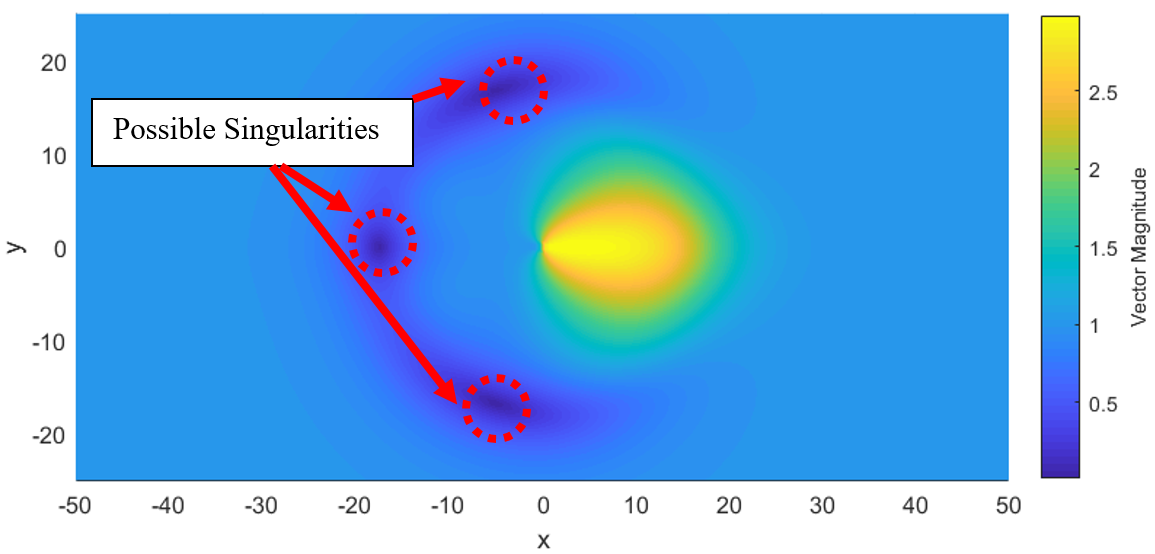
\includegraphics[trim=0 0 0 0,clip,width=14cm]{Figures/methods/summedHeatMapSimple2}
	\caption{Summed Fields Without Total Normalization}
	\label{fig:summedHeatMap}
\end{figure}

If singularities indicate possible trap situations, it is important to detect and avoid them. Singularities in the vector field are defined as a region in the GVF space where the vector has zero magnitude, shown in Equation \ref{eq:singularityCondition}.


\begin{equation}
\label{eq:singularityCondition}
||\overrightarrow{V}_g || = 0
\end{equation}

\noindent
By extension, singularities are a result of a zero vector, shown in Equation \ref{eq:zeroVectorCondition} and Equation \ref{eq:zeroVectorCondition2}.



\begin{equation}
\label{eq:zeroVectorCondition}
\overrightarrow{0} = \overrightarrow{V}_{||P||} +P\overrightarrow{V}_{||O||}
\end{equation}

\begin{equation}
\label{eq:zeroVectorCondition2}
\overrightarrow{V}_{||P||}=-P\overrightarrow{V}_{||O||}
\end{equation}

Vectors $\overrightarrow{V}_{||P||}$ and $\overrightarrow{V}_{||O||}$ are normalized, meaning that their magnitudes are of equal length $||\overrightarrow{V}_{||P||}||=||\overrightarrow{V}_{||O||}||$. For the condition shown in Equation \ref{eq:zeroVectorCondition2} to be true for an obstacle field with a negative convergence weight $G=-1$, the decay function $P$ must be unity. Setting Equation \ref{eq:decay} equal to $1$, the distance at which the fields have equal strength, and therefore possible singularity locations, is determined to be that shown in Equation \ref{eq:equalStrength}

\begin{equation}
\label{eq:equalStrength}
d = \frac{R}{2}
\end{equation}

Searching the GVF for locations that satisfy Equation \ref{eq:singularityCondition} can be accomplished numerically, however a good initial condition is necessary. Initial conditions placed at the radius of equal strength, defined by Equation \ref{eq:equalStrength}, on the side of the obstacle where deconstruction summation occurs the singularities can be found. Solving for the singularity locations with initial conditions placed evenly on the left hand side of the obstacle of the above scenario locates three singularities located on the radius of equation strength, shown in Figure \ref{fig:noCircSingularityDetection}.

\begin{figure}[H]
	\begin{subfigmatrix}{2}% number of columns
		\centering	
		\subfigure []{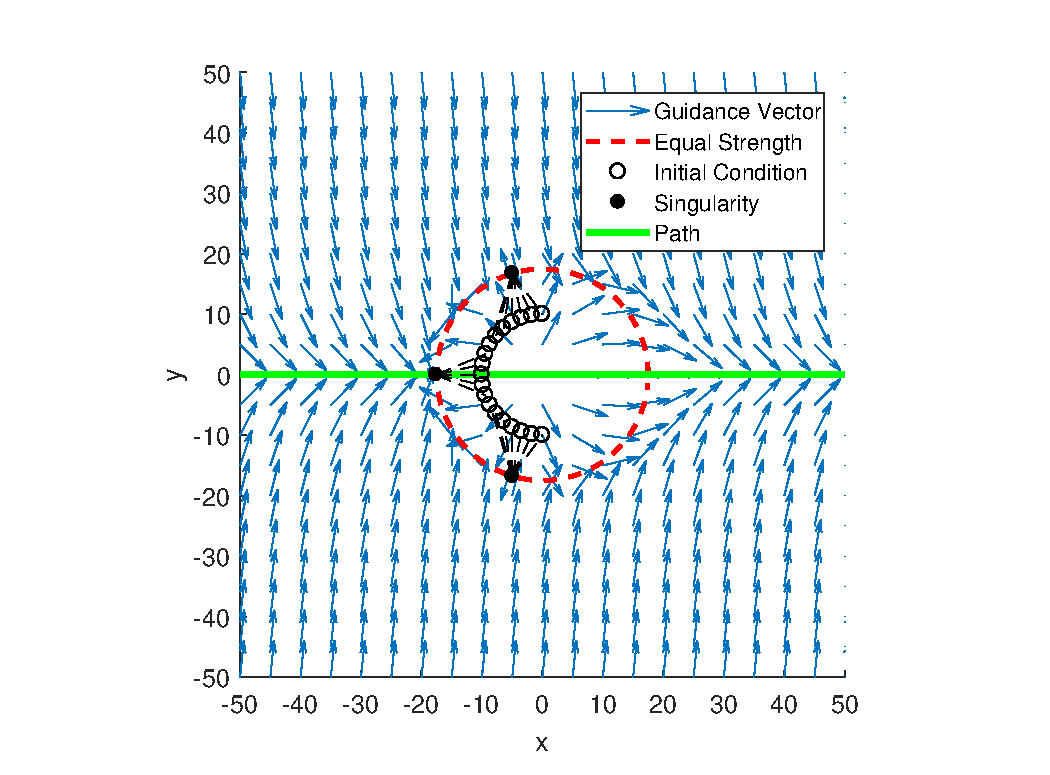
\includegraphics[trim=70 0 80 0,clip,width=7cm] {Figures/methods/noCircSingularityR10}}
		\subfigure []{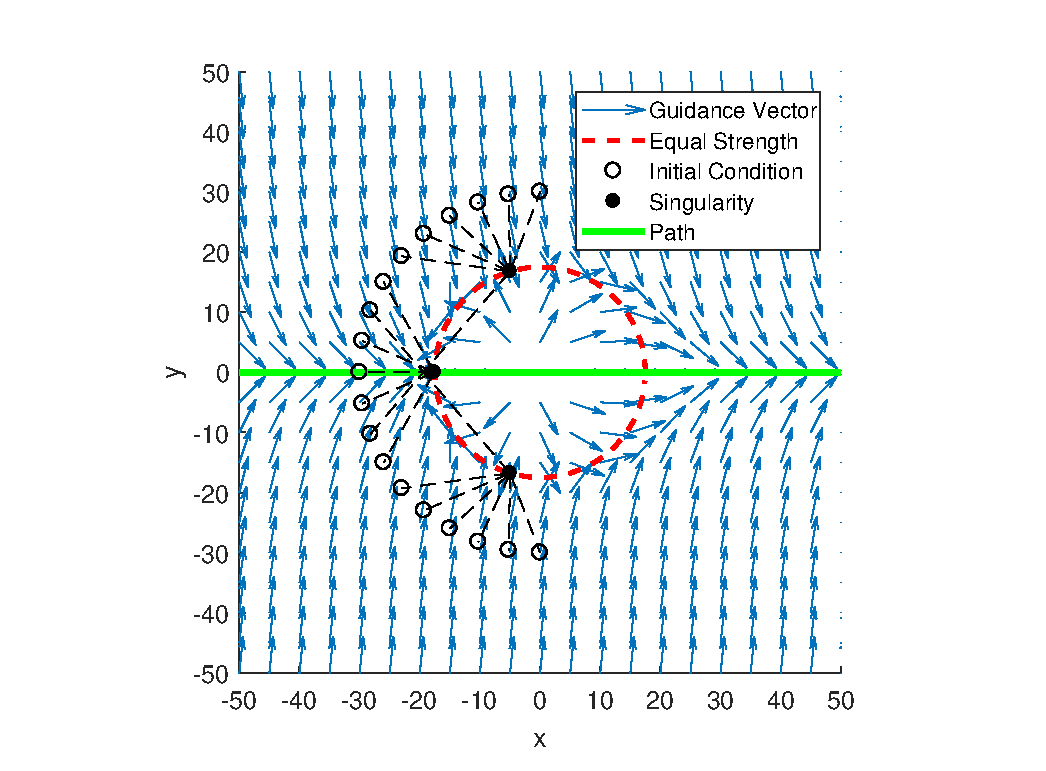
\includegraphics[trim=70 0 80 0,clip,width=7cm] {Figures/methods/noCircSingularityR30}}
		\hspace*{0mm}
	\end{subfigmatrix}
	\caption{GVF Converging and Circulating a Circular Path}
	\label{fig:noCircSingularityDetection}
\end{figure}

Singularities are caused by the two vector fields directly opposing each other, described in Equation \ref{eq:zeroVectorCondition2}. Adding circulation to the repulsive GVF may prevent the summed vectors from canceling out completely. To demonstrate the prevention of vector cancellation, the above scenario is repeated with equal magnitude convergence and circulation components. Note that by adding circulation to the obstacle vector field singularities are prevented from forming along the route the UAV is likely to take, shown in Figure \ref{fig:summedfieldscircsingularity}. Additionally, adding circulation provides a deterministic guidance on how to circumnavigate an obstacle. In literature, obstacles directed the UAV away and relied on the path following field for direction. 

\begin{figure}
	\centering
	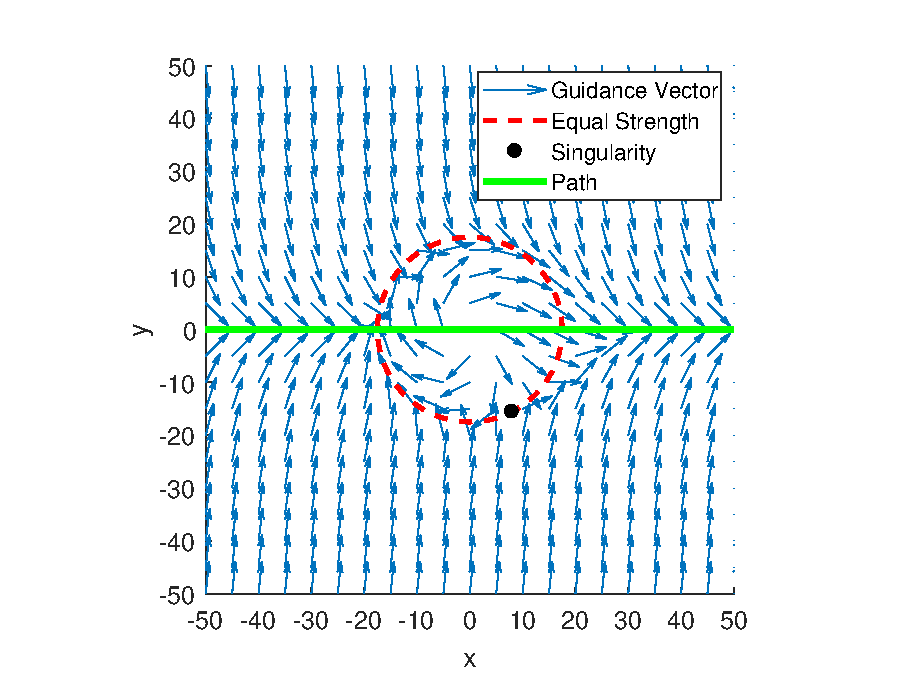
\includegraphics[width=12cm]{PaperFigures/Methods/summedFieldsCircSingularity}
	\caption{Singularity in Summed Field with Equal Magnitude Convergence and Circulation}
	\label{fig:summedfieldscircsingularity}
\end{figure}



\section{Phase II: Optimization of Obstacle Field}
\textbf{The objective of Phase II was to determine a combination of GVF circulation and decay radius for an optimized circular obstacle avoidance.} Demonstration of a UAV modeled as a Dubin's vehicle with maximum turn rate constraints converging and following a straight path for various target path circulations was provided. A circular obstacle represented by a strictly repulsive GVF was added to the path and the avoidance observed. Obstacles radius and their associated GVF decay radius were represented in terms of the UAVs turning radius for convenience. Next, a path deviation cost function was described and was to minimized to provide an optimized GVF obstacle avoidance guidance. Reduction in path deviation cost was achieved for a worst-case obstacle avoidance scenario presented. Lastly, a method for solving circulation and decay radius numerically was presented. 


\subsection{Vehicle and Obstacle Definition}

As discussed in literature and Phase I, GVF can be used to guide a UAV to converge and circulate a path. An example of a UAV traveling at constant speed $u=20m/s$ and fixed turn rate $\dot{\theta}=20deg/s$ converging and circulating a straight path using the GVF guidance described in Phase I is shown in Figure \ref{fig:uavPathFollowDemo}. Starting at an initial position of $(-45,20) \ m$ and heading $\theta$ of $45^\circ$, the UAV is shown converging and following a straight GVF path with weights $G=1,H=5$.


\begin{figure}[H]
	\centering
	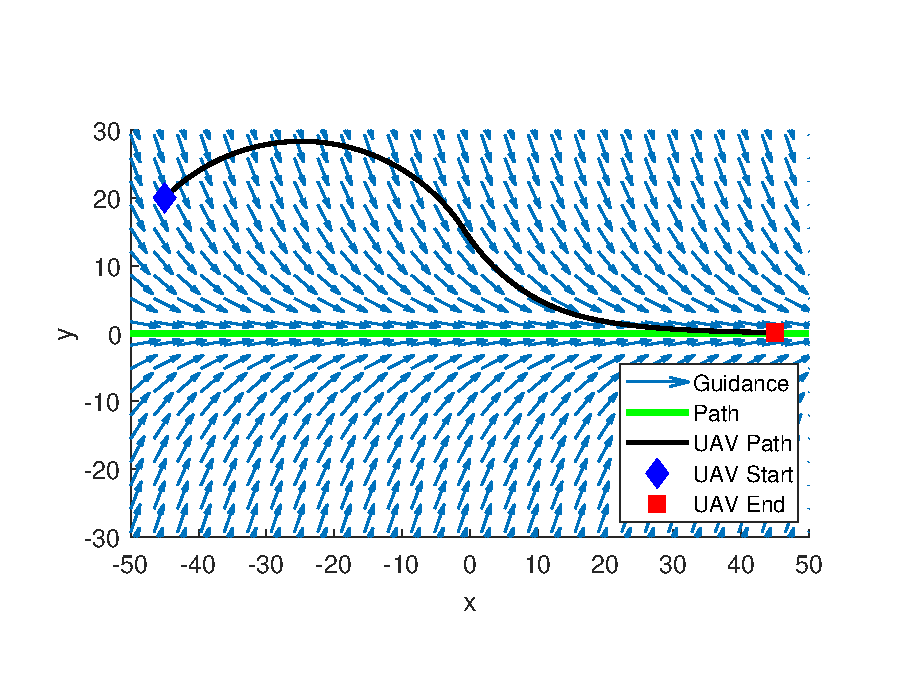
\includegraphics[trim=0 25 0 45,clip,width=14cm]{PaperFigures/Methods/uavPathFollowDemo}
	\caption{Fixed Wing Converging and Following a Path Simulation}
	\label{fig:uavPathFollowDemo}
\end{figure}

The effect of modifying $G$ and $H$ has not been well documented in literature when the GVF is normalized for a heading guidance. Various path circulation weights for a fixed UAV velocity were conducted and the lateral error with respect to time recorded to determine an appropriate relationship between circulation and UAV velocity. Increased circulation results in the vector field transitioning to path following more quickly. Low circulation weights allows convergence to dominate closer to the path. The UAV's route for converging and following a path with $G=1$ and multiple path circulation weights $H$ is shown in Figure \ref{fig:uavPathMultipleHs}. Low circulation results in a UAV route that quickly approaches the path, however begins to oscillate and has a larger stead-state error compared to fields with larger circulation. The largest circulation field $H=50$, does not oscillate, but takes considerably longer to converge. Circulation approximately the same value as the UAV's velocity results in a compromise between fast convergence and no oscillation. The lateral error from the path is shown in Figure \ref{fig:uavPathMultipleHsLateral}. 


\begin{figure}[H]
	\centering
	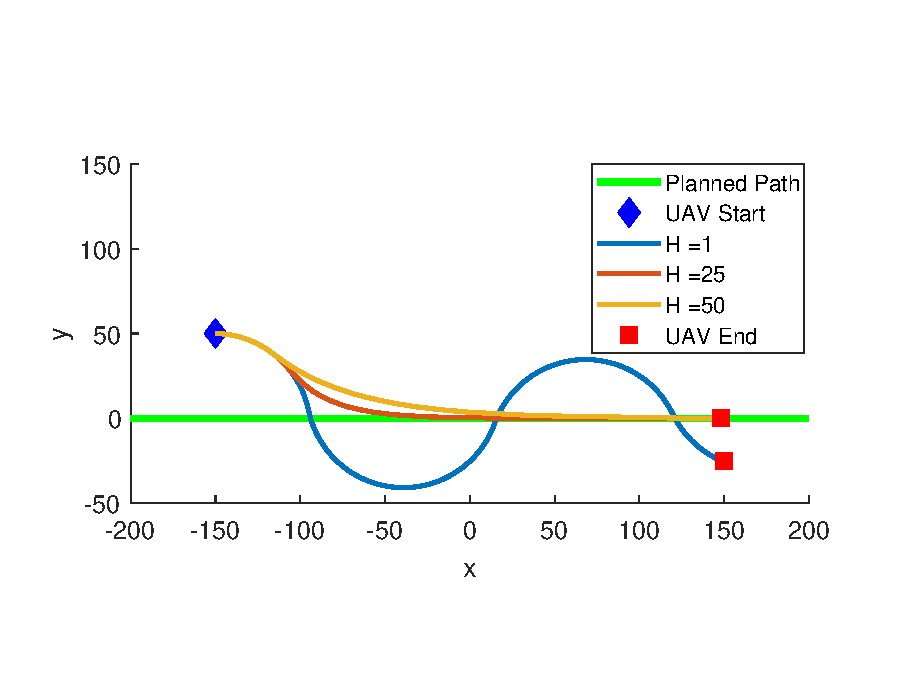
\includegraphics[trim=0 30 0 65,clip,width=14cm]{PaperFigures/Methods/pathMultipleHs}
	\caption{Fixed Wing Converging and Following a Path}
	\label{fig:uavPathMultipleHs}
\end{figure}


\begin{figure}[H]
	\centering
	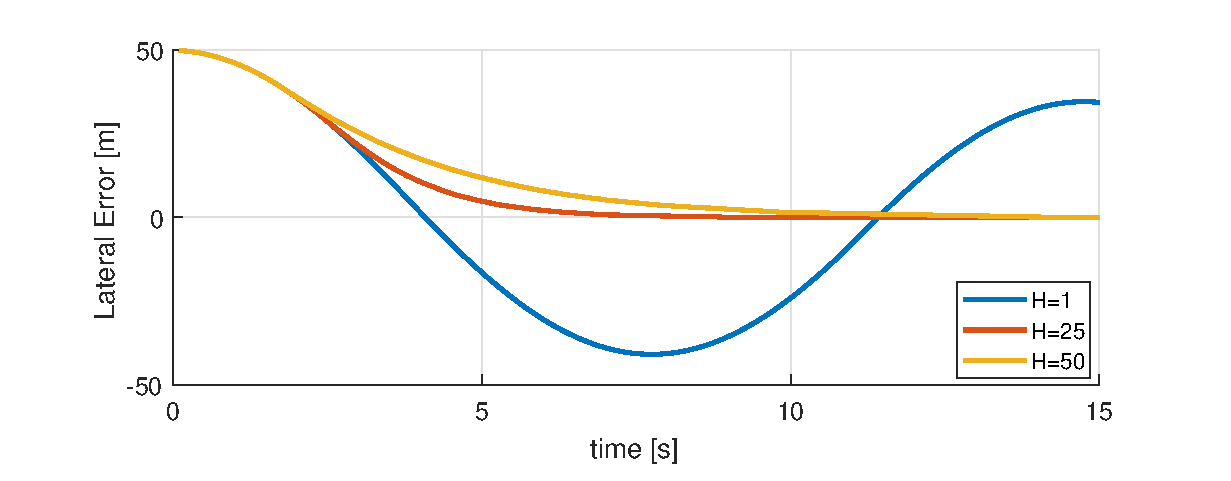
\includegraphics[trim=0 0 0 0,clip,width=16cm]{PaperFigures/Methods/lateralErrorVsTime}
	\caption{Lateral Error for Fixed Wing Guided by GVF Guidance of Multiple Circulations}
	\label{fig:uavPathMultipleHsLateral}
\end{figure}

From the above simulation it is observed that a circulation near the UAVs velocity provides a flight route that is a compromise between the high oscillation and high overshoot of a circulation $H=1$ while not having a longer settling time with high circulation $H=50$. For future simulations the circulation of the path following guidance will be assumed to be equal to that of the UAVs velocity, $H=u$. \\

\subsection{Obstacle on Planned Path}
As the UAV travels the path using GVF guidance, an obstacle may be encountered that, without intervention, the UAV may collide with. Obstacles along the pre-planned path are described using two parameters, the obstacle radius $r_o$ and the lateral distance from the path $y_o$. Representing the obstacle's position with respect to the path is convenient because it allows for a single optimized GVF solution to be applicable for multiple path angles $\delta$.

\begin{figure}[H]
	\centering
	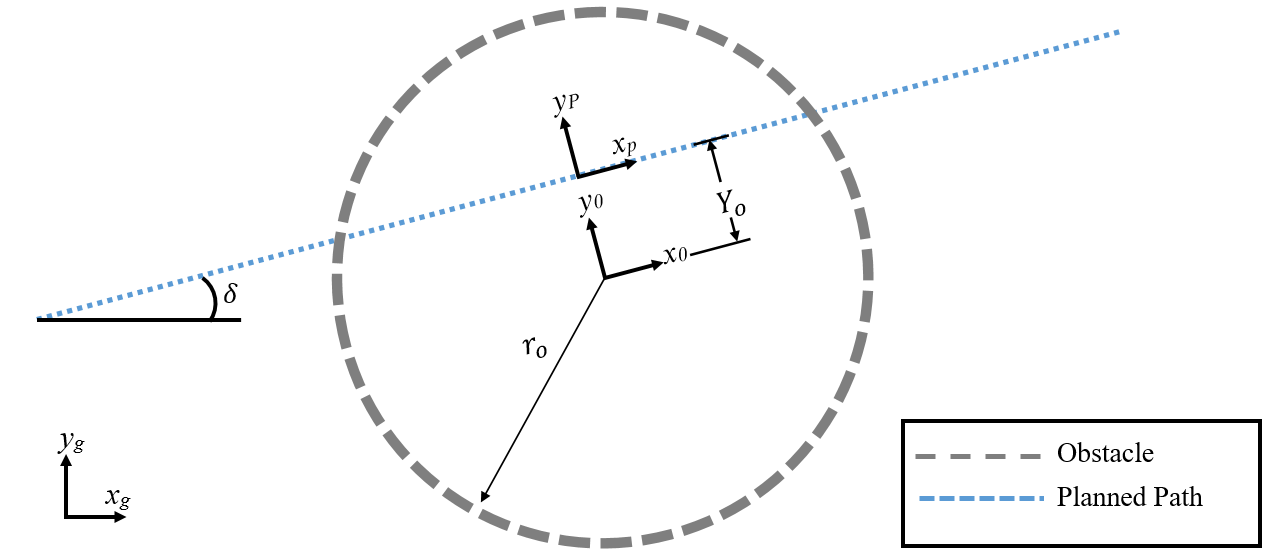
\includegraphics[width=14cm]{Figures/methods/obstacleOnPath}
	\caption{Circular Obstacle Along Planned Path}
	\label{fig:obstacleonpath}
\end{figure}

 It is assumed here that the radius of the obstacle is no smaller than the turn radius of the UAV $\theta_r$, which is calculated in Equation \ref{eq:turning_radius}. The obstacles radius and lateral position can be expressed in terms of the UAVs turning radius by the ratios $m$ and $c$ shown in Equations \ref{eq:obstR} and \ref{eq:obstC} respectively. Representing the obstacle by these ratios is convenient because it allows for a single set of optimized parameters to be used for a UAV of multiple velocities. 
 


\begin{equation}
\label{eq:turning_radius}
\theta_r = \frac{u}{\dot{\theta}}
\end{equation}

\begin{equation}
\label{eq:obstR}
r_o = m \theta_r
\end{equation}

\begin{equation}
\label{eq:obstC}
Y_o = c \theta_r
\end{equation}

The decay radius of the repulsive vector field, $R$, was defined in $k$ multiples of the obstacle's radius, shown in Equation \ref{eq:decayR}. 
 
 \begin{equation}
 \label{eq:decayR}
 R = k r_o
 \end{equation}
 
 

 A cost function can be used to measure the deviation from a planned path while avoiding an obstacle with GVF in Equation \ref{eq:staticCost}. The lateral distance of the UAV to the planned path was represented by $y$ and $r_o$ is the obstacle radius.
 
 \begin{equation}
 \label{eq:staticCost}
 \gamma = \frac{1}{r_o}\int_{0}^{tf}ydt
 \end{equation}
 
 
 Strictly repulsive GVF obstacle fields can provide avoidance, however may cause excess deviation from the pre-planned path, cause unnecessary turns, and flight routes near or through guidance singularities. A UAV traveling at a speed of $10m/s$ and a turn rate of $20 deg/s$ is given a summed path following and obstacle avoidance guidance $\overrightarrow{V}_g$, defined in Equation \ref{eq:totalGuidance} in Phase I. An obstacle centered on the path $y_o=0$ and radius $r_0 = \theta_r$ is to be avoided. The decay radius multiplier $k$ was increased manually over several simulations until avoidance was achieved. The flight path of the UAV with summed guidance is shown in Figure \ref{fig:uavPathObstNoCirc}. The UAV experiences excessive path deviation and takes considerable time to settle back to the planned path. Additionally, the guidance directs the UAV to pass directly through a singularity and passes near an additional singularity towards the top of the obstacle. The cost, calculated from Equation \ref{eq:staticCost}, for avoidance using the strictly repulsive guidance for head on collision scenario is $\gamma=25$.
 

\begin{figure}[H]
	\centering
	%Simulations performed with findSingularities.m
	%G=-1,H=0, n = 1.5,k=2.8
	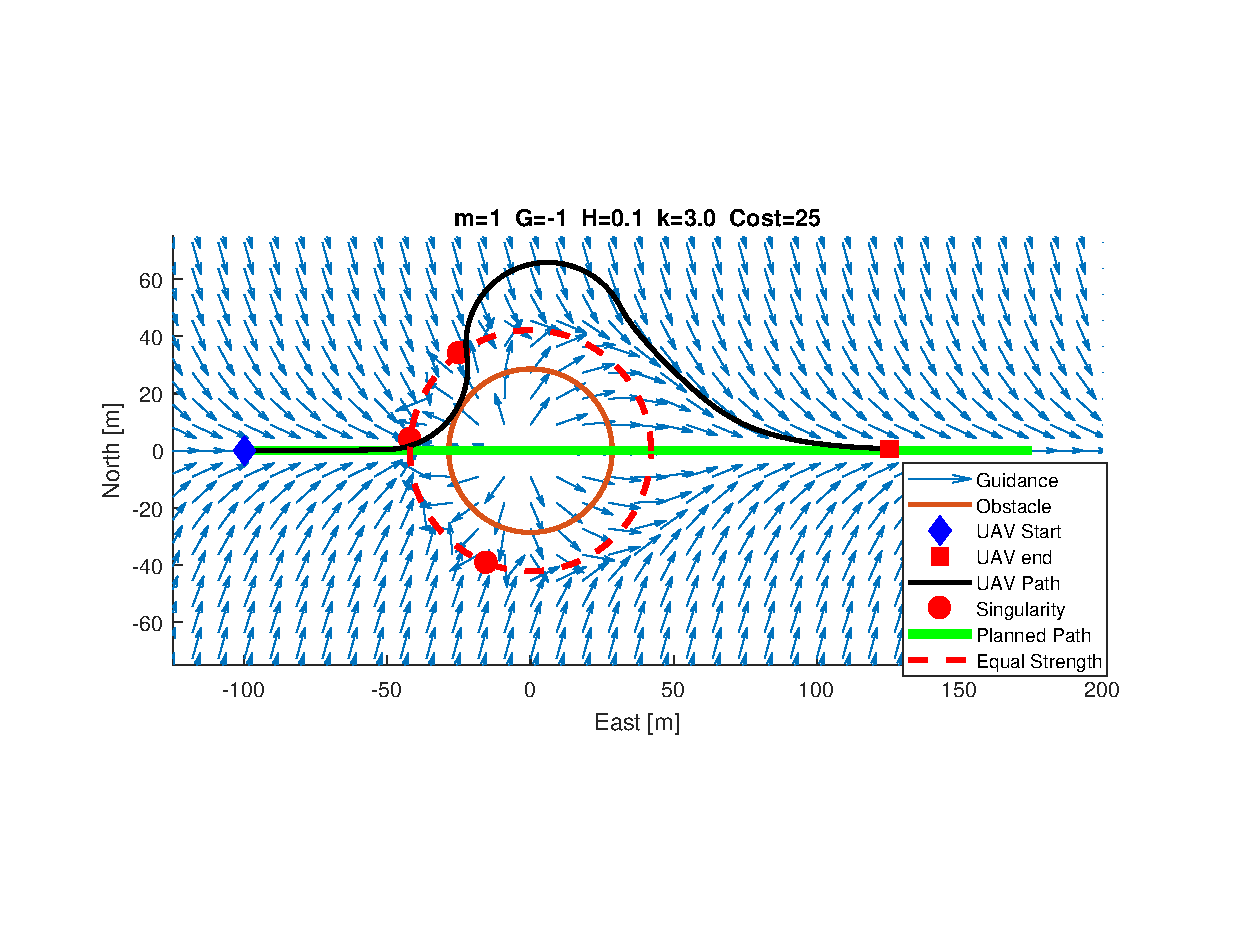
\includegraphics[trim=0 85 0 85,clip,width=15cm]{PaperFigures/Methods/bruteForceSolveN1V10}
	\caption{UAV Encountering a Circular Obstacle Centered on Pre-planned Path, No Circulation}
	\label{fig:uavPathObstNoCirc}
\end{figure}

Adding circulation to the obstacle guidance $\overrightarrow{V}_o$, as described in Phase I, may remove singularities from the UAVs route and reduce deviation from the planned path. Additionally, circulation adds deterministic information on how to circumnavigate an obstacle whereas strictly repulsive fields rely on the path following field to determine circumnavigation direction. Equal magnitudes convergence $G_o$ and circulation $H_o$ removes the guidance singularities from the UAV's path, adds a more gentle transition between fields shown in Figure \ref{fig:uavPathObstWithCirc}. The cost of the head on collision avoidance using GVF guidance with obstacle circulation results in a cost of $\gamma=7$.



\begin{figure}[H]
	\centering
	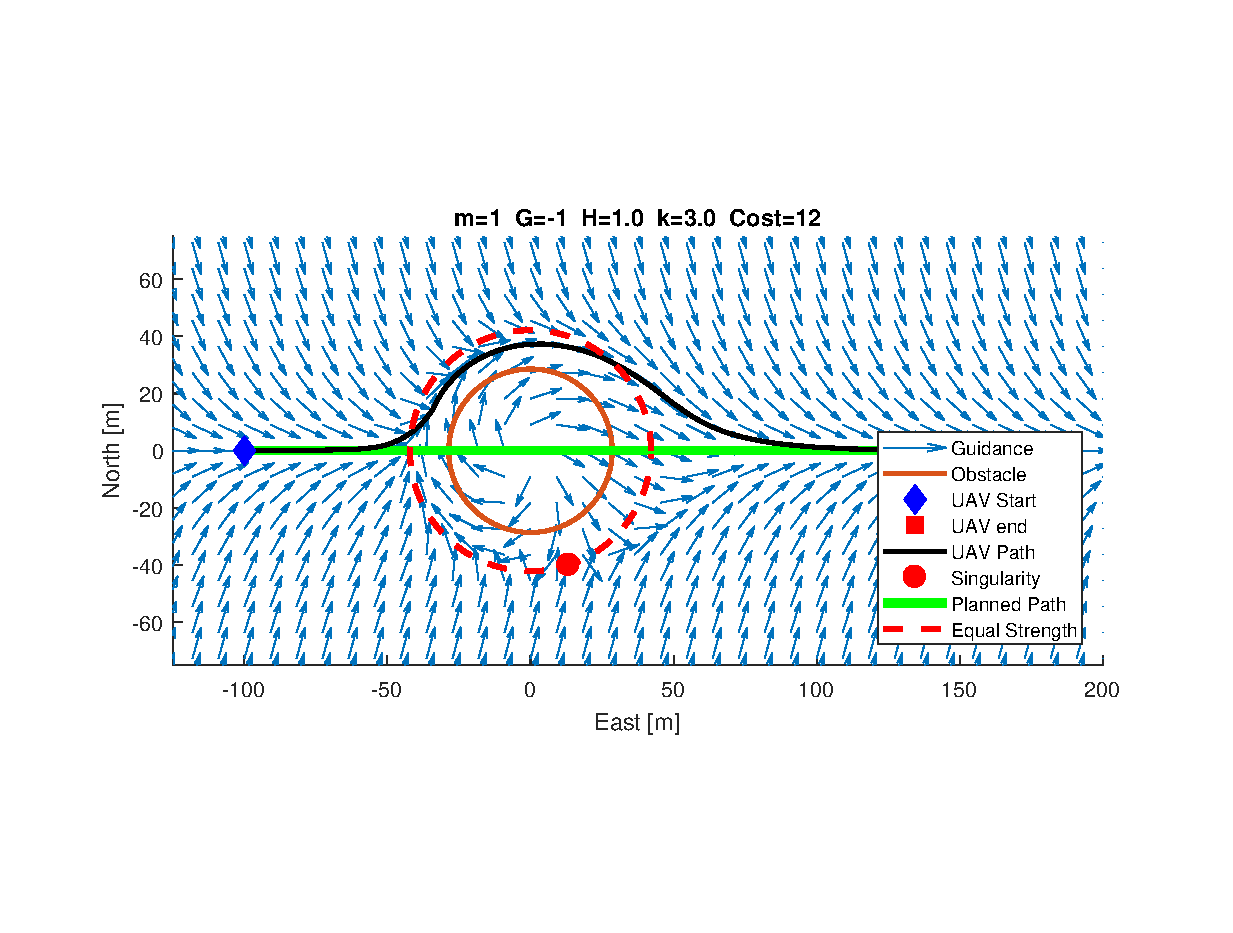
\includegraphics[trim=0 85 0 85,clip,width=15cm]{PaperFigures/Methods/bruteForceSolvedN1V10WithCirc}
	\caption{UAV Encountering a Circular Obstacle Centered on Pre-planned Path with Circulation}
	\label{fig:uavPathObstWithCirc}
\end{figure}

Adding equal magnitude parts $G$ and $H$ produce guidance with a $70 \%$ lower cost compared to strictly repulsive, however, $k$ and $H$ should be selected such that the cost is minimized. One method for selecting decay field radius and circulation parameters is to evaluate a large range of parameters and observe the cost for avoidance with each combination. The cost function shown in Equation \ref{eq:staticCost} only penalized the UAV for path deviation, however should be modified to also be penalized for violating the obstacle space. The new cost function $\bar{\gamma}$ adds an additional piecewise function which increases the cost if the UAV is inside or on the obstacle's edge, shown in Equation \ref{eq:staticCostWithObst}


 \begin{equation}
\label{eq:staticCostWithObst}
\bar{\gamma} = \frac{1}{r_o}\int_{0}^{tf}ydt + j(x,y)
\end{equation}

\begin{equation}
j(x,y) = \left\{
\begin{array}{ll}
100dt & \quad \sqrt{(x-xc)^2+(y-yc)^2} \leq r_O \\
0 & \quad \sqrt{ (x-xc)^2+(y-yc)^2 } > r_O
\end{array}
\right.
\end{equation}


Using the above cost function $\bar{\gamma}$ in the same scenario presented in Figure \ref{fig:uavPathObstNoCirc}, several simulations were conducted with identical UAV parameters and obstacle radius $r_o$ with varying $k$ and $H_o$ values. The cost of each simulation is shown in the heatmap in Figure \ref{fig:costHandR}. 

\begin{figure}[H]
	\centering
	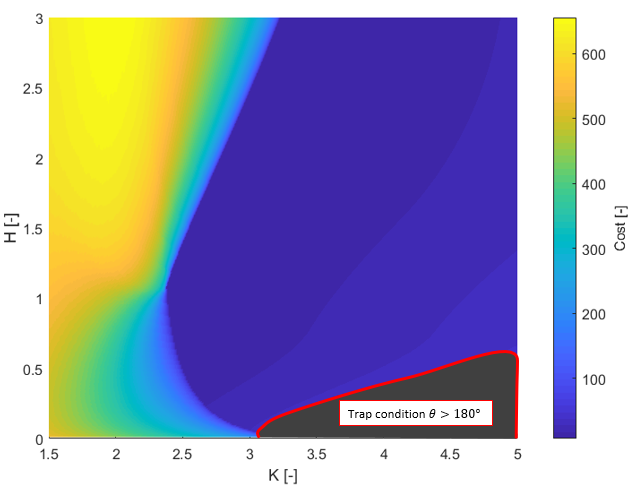
\includegraphics[trim=0 0 0 10,clip,width=16cm]{PaperFigures/Methods/costHandRwithTrap.png}
	\caption{Heatmap of Cost as Function of $k$ and $H_o$}
	\label{fig:costHandR}
\end{figure}

Finding the minimum cost of the above heatmap and looking up the corresponding $k$ and $H_o$ values at which the minimum occurs can be used to provide an optimized avoidance. Solving the desired parameters for an optimal guidance using this search method for the general case is computationally expensive and can take many hundreds of simulations to evaluate the desired space. The problem becomes one of minimization of the cost function and to find a solution numerically without solving for a large range of parameters, shown in Equation \ref{eq:minimizer}.

\begin{equation}
\label{eq:minimizer}
\begin{aligned}
& \underset{H,k}{\text{minimize}}
& & \frac{1}{r_o}\int_{0}^{tf}ydt + j(x,y) 
\end{aligned}
\end{equation}

A numerical solver which attempts to minimize a given cost function can be found in MATLAB called $fmincon()$. The minimizer operates on the following principle. Provided an initial condition array $X_I$, minimize the function $\bar{\gamma}$ by observing the change in $\bar{\gamma}$ within certain bounds. The reduction in cost as the minimizer runs is shown in Figure \ref{fig:finalfunctionvalue}.

\begin{figure}[H]
	\centering
	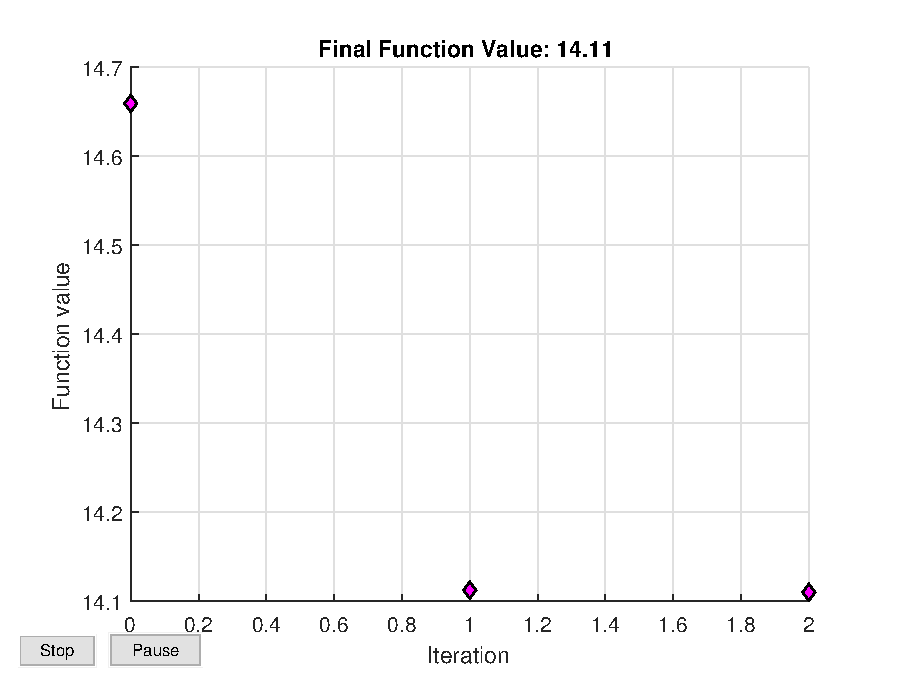
\includegraphics[width=12cm]{PaperFigures/Methods/finalFunctionValue}
	\caption{Cost Function Reduction in fmincon() MATLAB Function}
	\label{fig:finalfunctionvalue}
\end{figure}

The optimizer found a solution combination of $k=2.7$ and $H_o = 1.8$ and results in a path with cost $\bar{\gamma}=14$. The path can be seen below in Figure \ref{fig:optimizedPath}.

\begin{figure}[H]
	\centering
	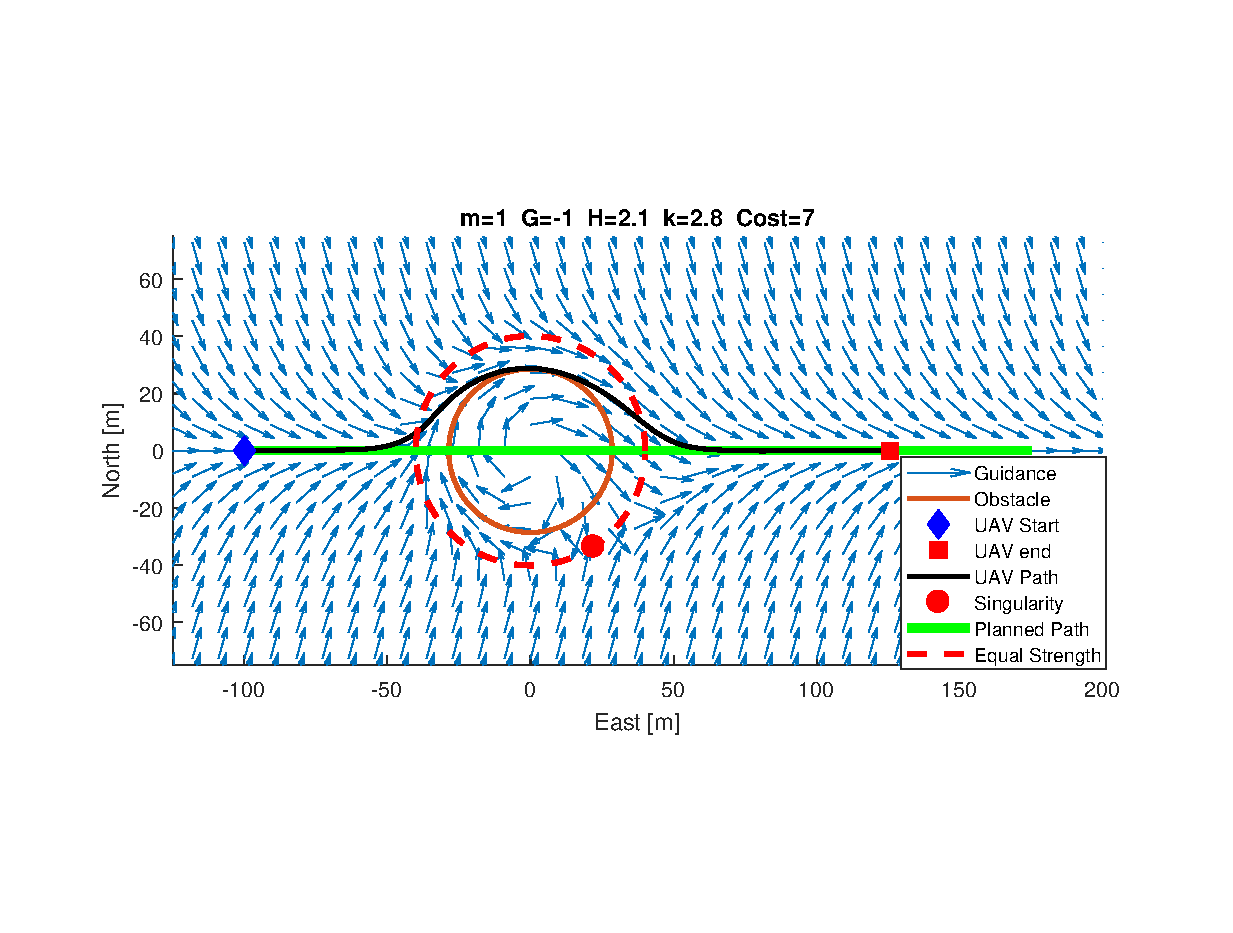
\includegraphics[trim=0 85 0 85,clip,width=15cm]{PaperFigures/Methods/solvedN1V10}
	\caption{UAV Path From Optimized GVF}
	\label{fig:optimizedPath}
\end{figure}


It was shown that avoidance can be achieved with a strictly repulsive GVF without the need to add circulation, however the simulated UAV encountered singularities along the route and had excess path deviation. Equal magnitudes convergence and circulation decreased the path deviation cost and no time was required to optimize the circulation weight. Searching the configuration space for a range of decay radius multipliers $k$ and obstacle circulation weights $H_o$ decreases the cost further compared to equal magnitude, however takes significant amount of time determine the cost for all combinations inside the configuration space. The optimized GVF guidance was shown to provide guidance with the same cost as the configuration space search with significantly reduced time from 10 hours to 5.2 seconds. All simulations were performed on an Intel i-7 7700k processor with 8Gb of ram. \\


Determining how GVF compares against other methods such as VFF, waypoint, and the optimal path around an obstacle is now discussed. A summary of the methods investigated for selecting GVF decay radius and circulation are shown in Table \ref{table:gvfMethodTable} below.




\begin{table}[]
	\centering
	\caption{Investigated Weighting Methods}
	\label{table:gvfMethodTable}
	\begin{tabular}{|l|l|l|}
		\hline
		GVF Method           & Cost {[}-{]} & Solve Time  \\ \hline
		Strictly Repulsive   & 25           & 0           \\ \hline
		Equal Magnitude      & 12           & 0           \\ \hline
		Configuration Search & 7            & 10.4 hours  \\ \hline
		Optimizer            & 7            & 5.2 seconds \\ \hline
	\end{tabular}
\end{table}



\subsection{Optimal Avoidance Route for Straight Path}
A geometrically optimal route around a circular obstacle can be used to compare the performance of avoidance algorithms. The path for avoiding a circular obstacle while minimizing path deviation can be accomplished with three circular arc turns. The first and third arc utilize the UAVs minimum turning radius, $\theta_r$, calculated in Equation \ref{eq:turnRadius}. The start of the first minimum radius turn begins when the UAV's horizontal position $x$ reaches  $\tilde{x}$ from the path frame origin. At a horizontal position $-\hat{x}$ the UAV turns with a radius of the obstacle $r_o$ and exits when the UAVs horizontal position reaches $\hat{x}$. 

\begin{equation}
\label{eq:turnRadius}
\theta_r = \frac{u}{\dot{\theta}}
\end{equation}

\noindent
The horizontal points $\tilde{x}$ and $\hat{x}$ are shown in Equations \ref{eq:optPathXtilde} and \ref{eq:optPathXhat}, respectively. 

\begin{equation}
\label{eq:optPathXtilde}
\widetilde{x} = -\sqrt{(\theta_r+R)^2 - (\theta_r-Y_o)^2}
\end{equation}

\begin{equation}
\label{eq:optPathXhat}
\hat{x} = \frac{R\sqrt{(r+R)^2-(\theta_r-Y_o)^2}}{R+\theta_r}
\end{equation}

\noindent
The avoidance path for navigating around a circular obstacle with minimum deviation from the planned path is defined in Equation \ref{eq:optPath} and shown in Figure \ref{fig:optimalpath}.


\begin{equation}
\label{eq:optPath}
y(x) = \left\{
\begin{array}{ll}
\widetilde{y} -\sqrt{\theta_r^2 - (x-\widetilde{x})^2} &  x < -\hat{x} \\
Y_o +\sqrt{R^2 - x^2} & -\hat{x} \leq x \geq \hat{x}\\
\widetilde{y} -\sqrt{\theta_r^2 - (x+\widetilde{x})^2}&  x > -\hat{x}
\end{array}
\right.
\end{equation}

\begin{figure}[H]
	\centering
	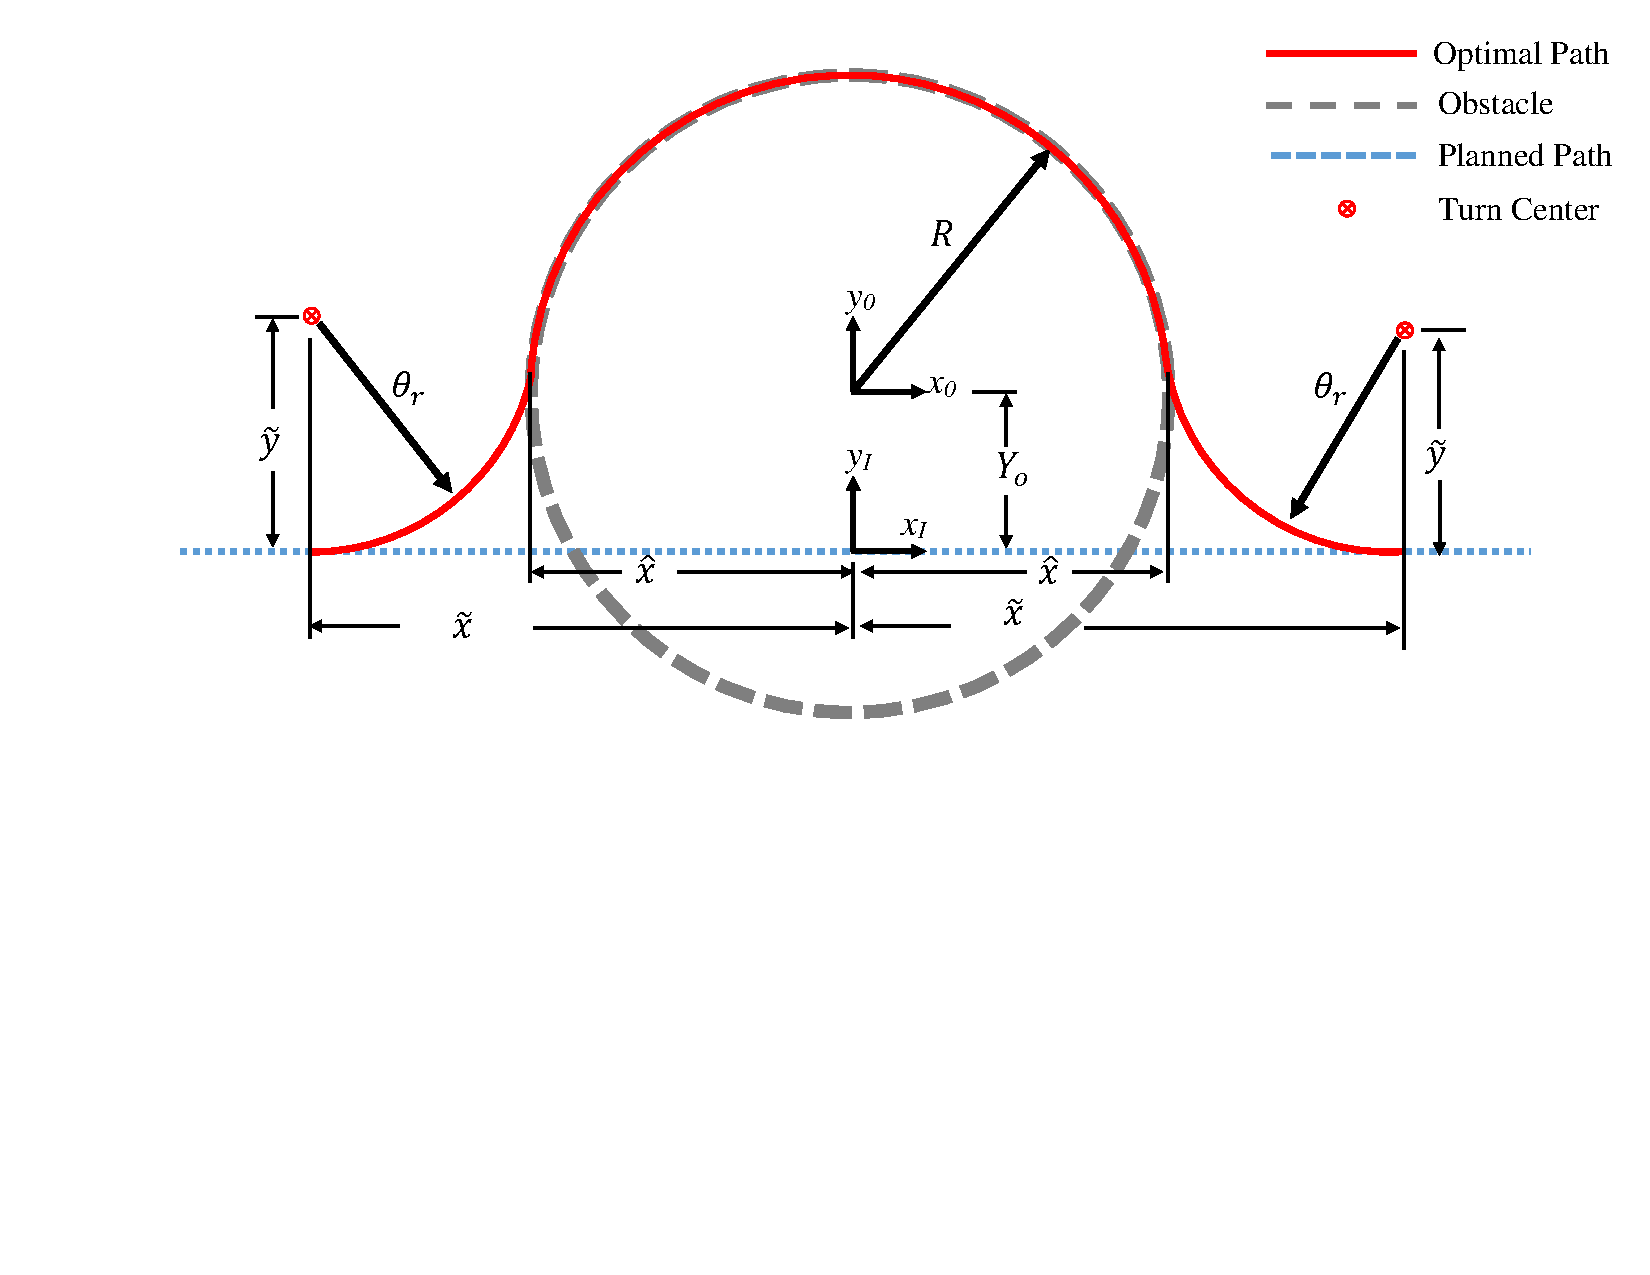
\includegraphics[width=0.7\linewidth ,trim=0 265 0 20,clip,width=15cm]{Figures/optimalPath/optimalPath}
	\caption{Optimal Kinematic Path Around Circular Obstacle}
	\label{fig:optimalpath}
\end{figure}


\subsection{Avoidance Path and Waypoints}

 The number of waypoints that divert around an obstacle effects how closely the UAV tracks the outside of the obstacle and how much of the original path can be traveled. Few obstacle diversion waypoints leads to excess path deviation while increasing the number of diversion waypoints reduces path deviation, however has diminishing returns. The cost function in Equation \ref{eq:staticCost} is used below to demonstrate how increasing the number of waypoints decreases the cost function, however, approaches an asymptote around six waypoints.


\begin{figure}[H]
	\begin{subfigmatrix}{2}% number of columns
		\centering	
		\subfigure []{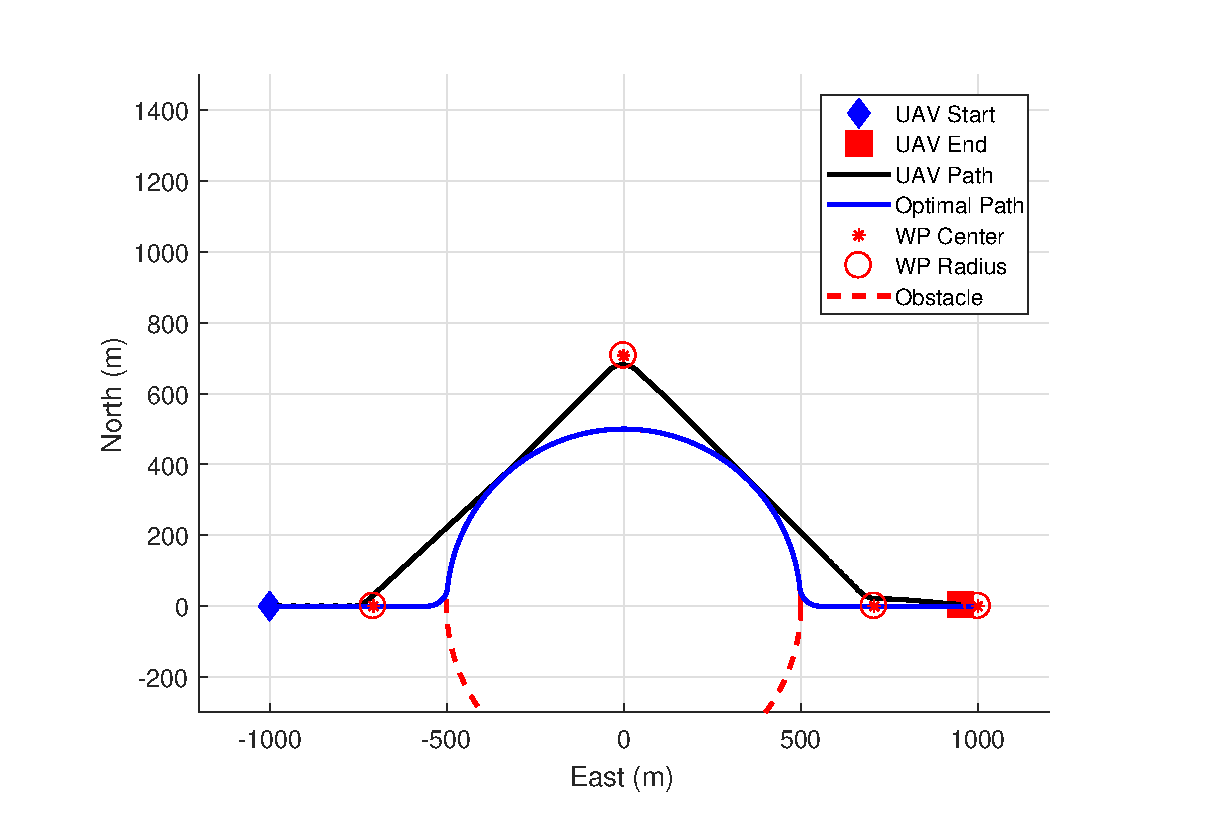
\includegraphics[width=7.5cm,trim=40 0 50 0,clip] {Figures/Waypoints/1Wpts}}
		\subfigure []{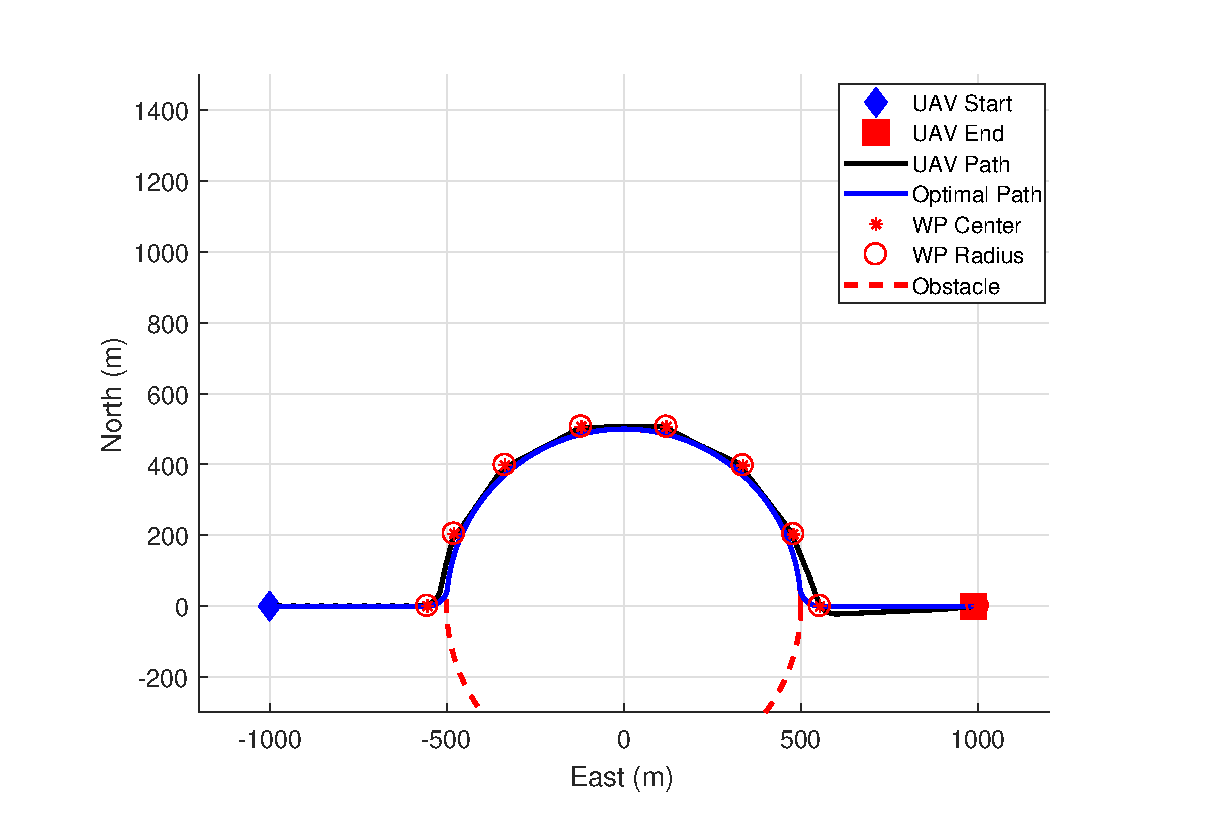
\includegraphics[width=7.5cm,trim=40 0 50 0,clip] {Figures/Waypoints/6Wpts}}
		\hspace*{0mm}
	\end{subfigmatrix}
	\caption{Obstacle Diversion Waypoints}
	\label{fig:numWaypointsPath}
\end{figure}

\begin{figure}[H]
	\centering
	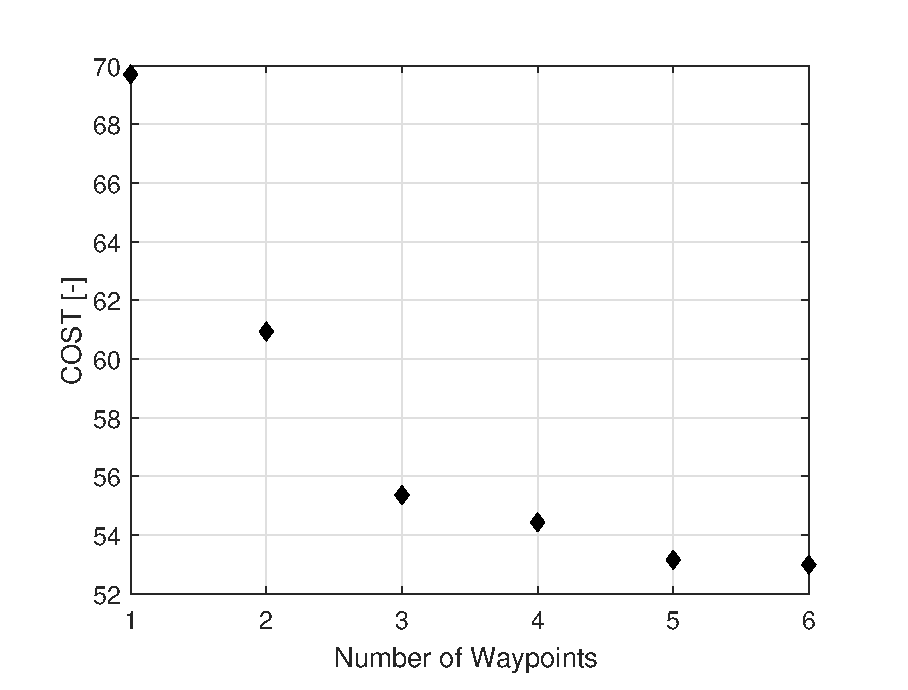
\includegraphics[width=10cm]{Figures/Waypoints/costVnumWpts}
	\caption{Cost Impact Versus Number of Waypoints}
	\label{fig:numWaypoints}
\end{figure}



\subsection{Circulation and Decay Lookup Tables}
Solving for optimized circulation and decay radius during flight may be problematic since the time to reach a solution increases with the size of the obstacle. Optimized GVF circulation and decay radius could be selected from a pre-computed lookup table in real time, removing the need to calculate the optimized parameters during flight. Lookup tables were generated by determining the optimized circulation and decay radius for a range of possible obstacle configurations. The obstacle's radius is again described in positive multiples of the UAVs turning radius, described in Equation \ref{eq:obstR}. It is also convenient to describe the obstacles lateral position to the path in terms of the UAV's turning radius by the multiple $c$ shown in Equation \ref{eq:latC}.

\begin{equation}
\label{eq:latC}
Y_o = c \theta_r
\end{equation}

Obstacle configurations were evaluated for a range of radii $m$ on the interval $[1,5]$ with a step size of 0.5 and lateral positions $c$ with an step size of 0.1. The UAV was assumed to travel at $10m/s$ with a maximum turn rate of $20 deg/s$ with a time step $dt$ of $0.01$ seconds. Lookup tables for obstacle field circulation $H_o$ and decay radius $k$ are shown in the heatmaps in Figures \ref{fig:htableheat} and \ref{fig:ktable} respectively. 

\begin{figure}[H]
	\centering
	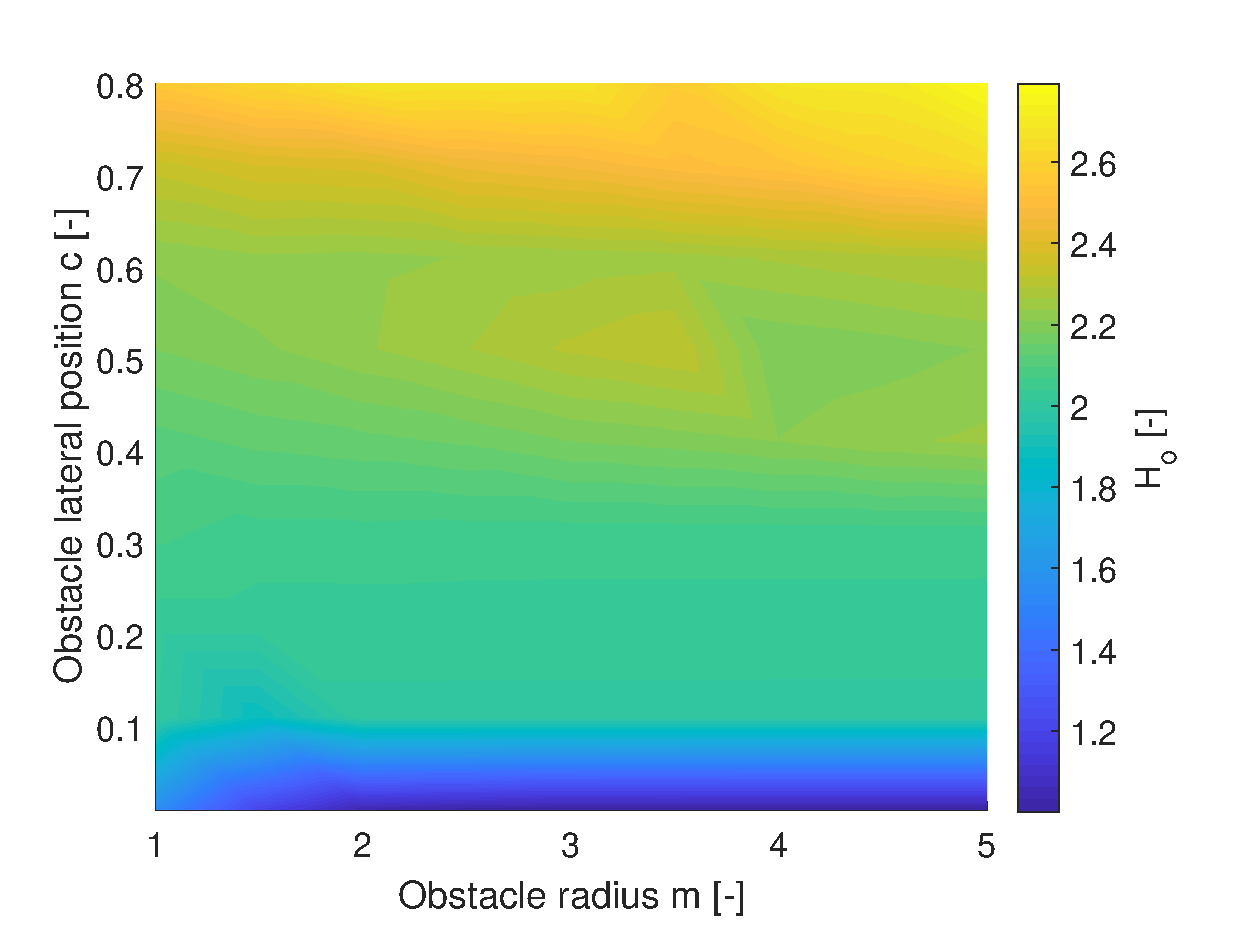
\includegraphics[width=10cm]{PaperFigures/Methods/LookupTable/hTableHeat}
	\caption{Obstacle Circulation Lookup Table, Smoothed by Interpolation}
	\label{fig:htableheat}
\end{figure}

\begin{figure}[H]
	\centering
	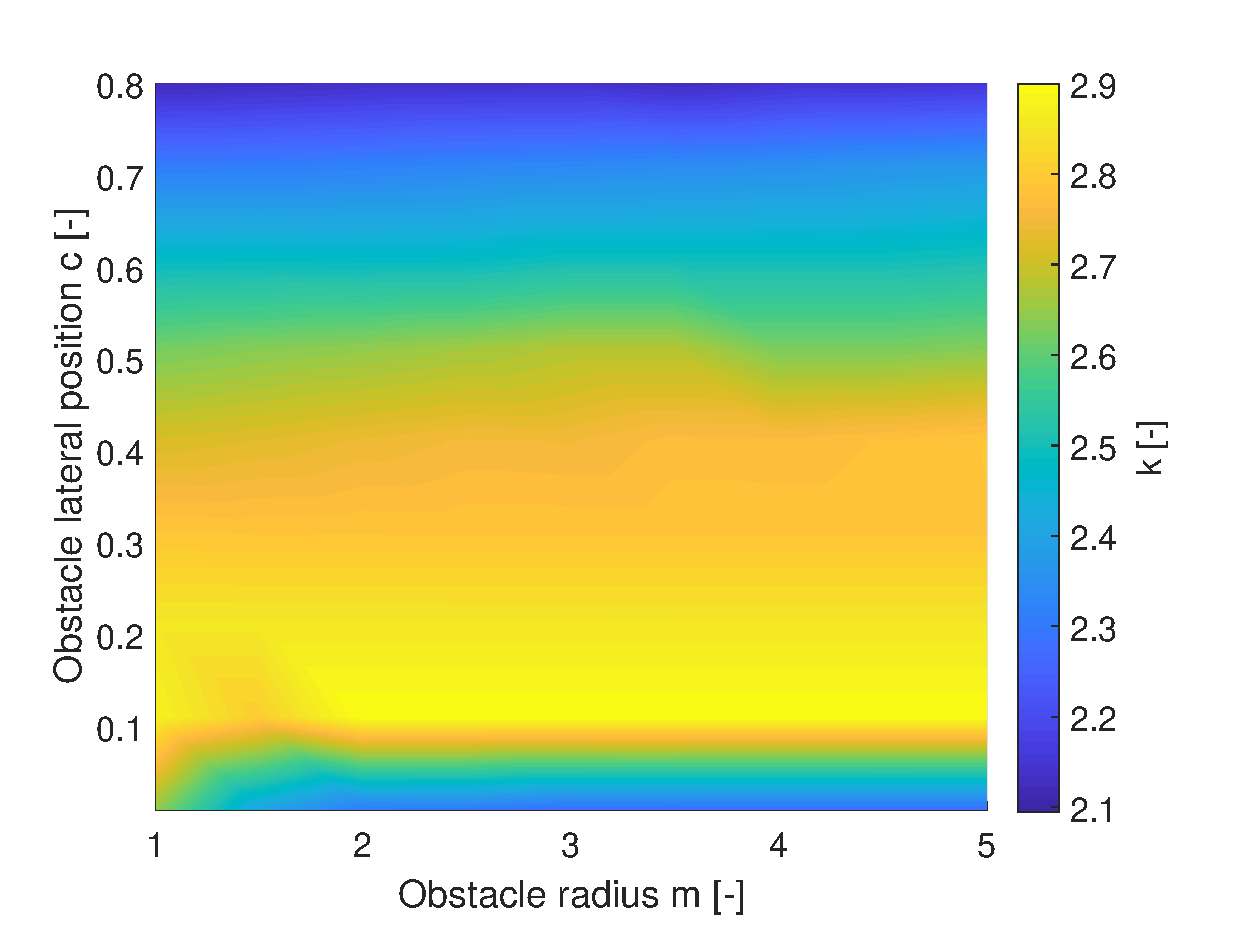
\includegraphics[width=10cm]{PaperFigures/Methods/LookupTable/kTableHeat}
	\caption{Obstacle Decay Radius Lookup Table, Smoothed by Interpolation}
	\label{fig:ktable}
\end{figure}

For obstacle configurations that were not optimized, circulation and decay radius may be determined by interpolation. To determine how the performance of interpolated solutions compare against an optimized solution, interpolation points were selected in a grid pattern between the tabulated values and the cost of each solution recorded. The interpolated points that were evaluated are shown in Figures \ref{fig:htableInterp} and \ref{fig:ktableInterp} below. 


\begin{figure}[H]
	\centering
	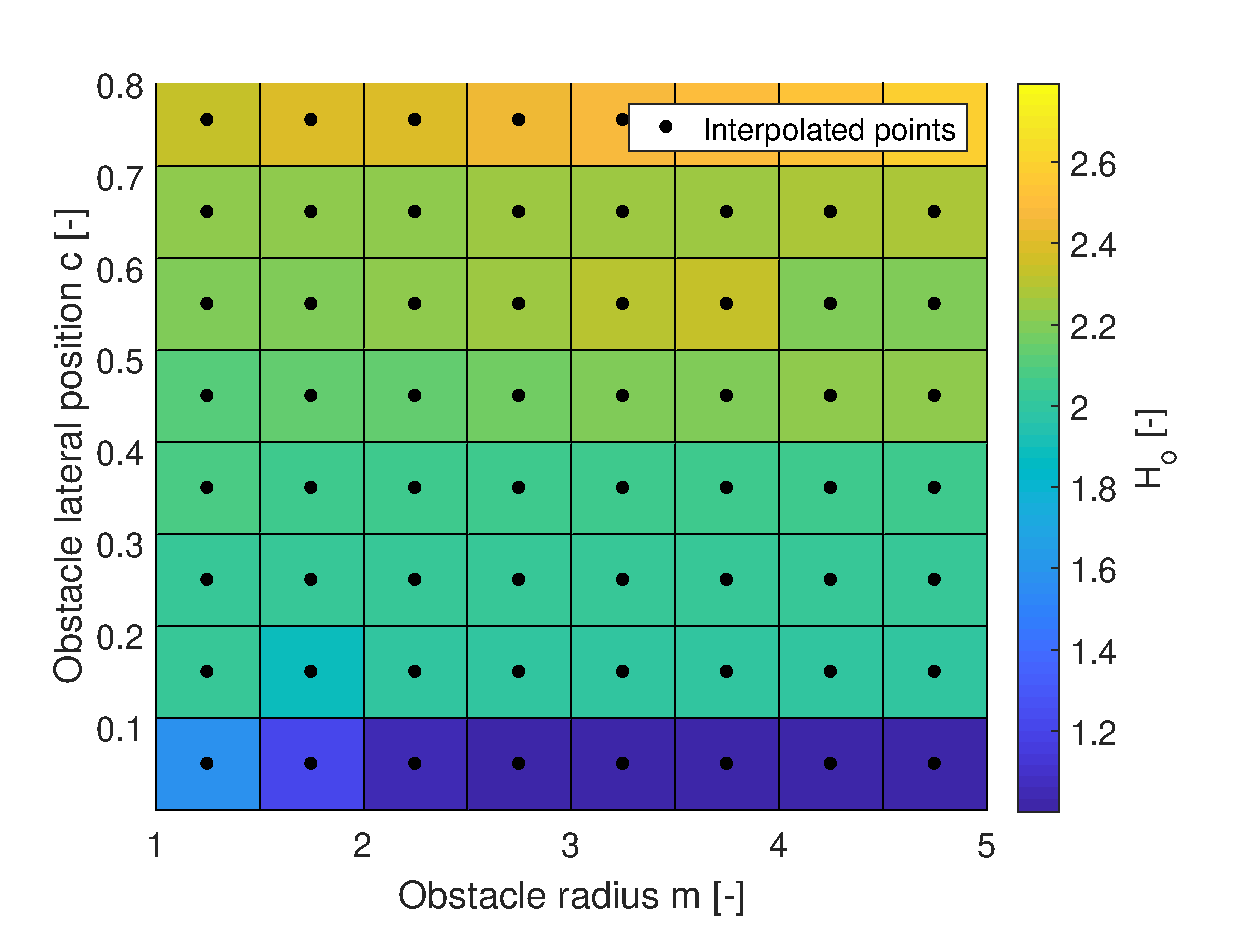
\includegraphics[width=12cm]{PaperFigures/Methods/LookupTable/hTableInterpolationPoints}
	\caption{Obstacle Circulation Lookup Table with Interpolation Points}
	\label{fig:htableInterp}
\end{figure}


\begin{figure}[H]
	\centering
	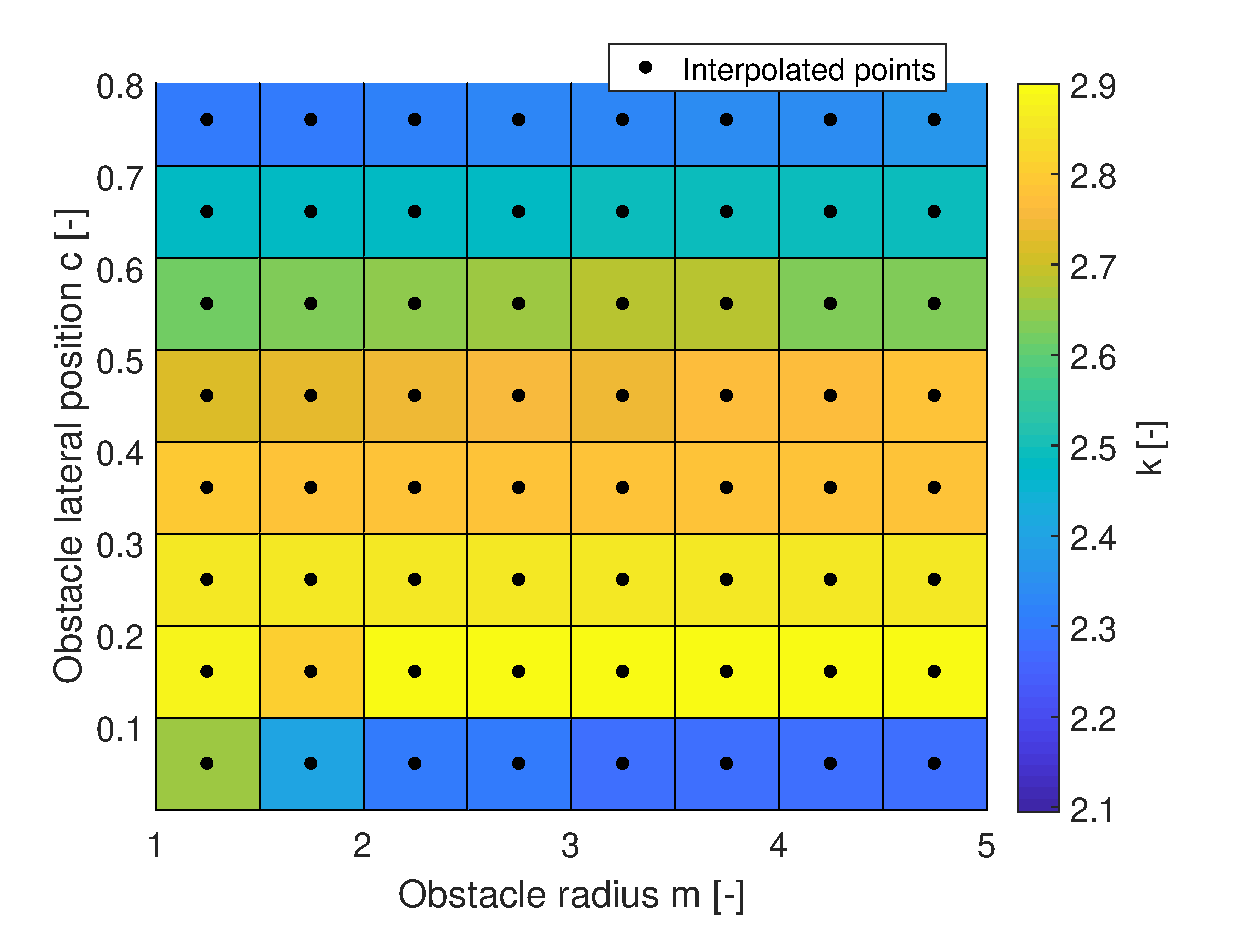
\includegraphics[width=12cm]{PaperFigures/Methods/LookupTable/kTableInterpolationPoints}
	\caption{Obstacle Decay Radius Lookup Table with Interpolation Points}
	\label{fig:ktableInterp}
\end{figure}

The cost of optimized versus the cost of interpolated solutions are represented as two planes overlaid in Figure \ref{fig:costplanes} below. The interpolated solution resembles the same behavior as the optimized solution, and for the configuration evaluated has a mean square error of $2.5$. Expressing the obstacle's radius and lateral position in terms of positive multipliers of the UAV's turning radius allows a single lookup table to be used for multiple UAV speeds, resulting in less scenarios to be evaluated.

\begin{figure}[H]
	\centering
	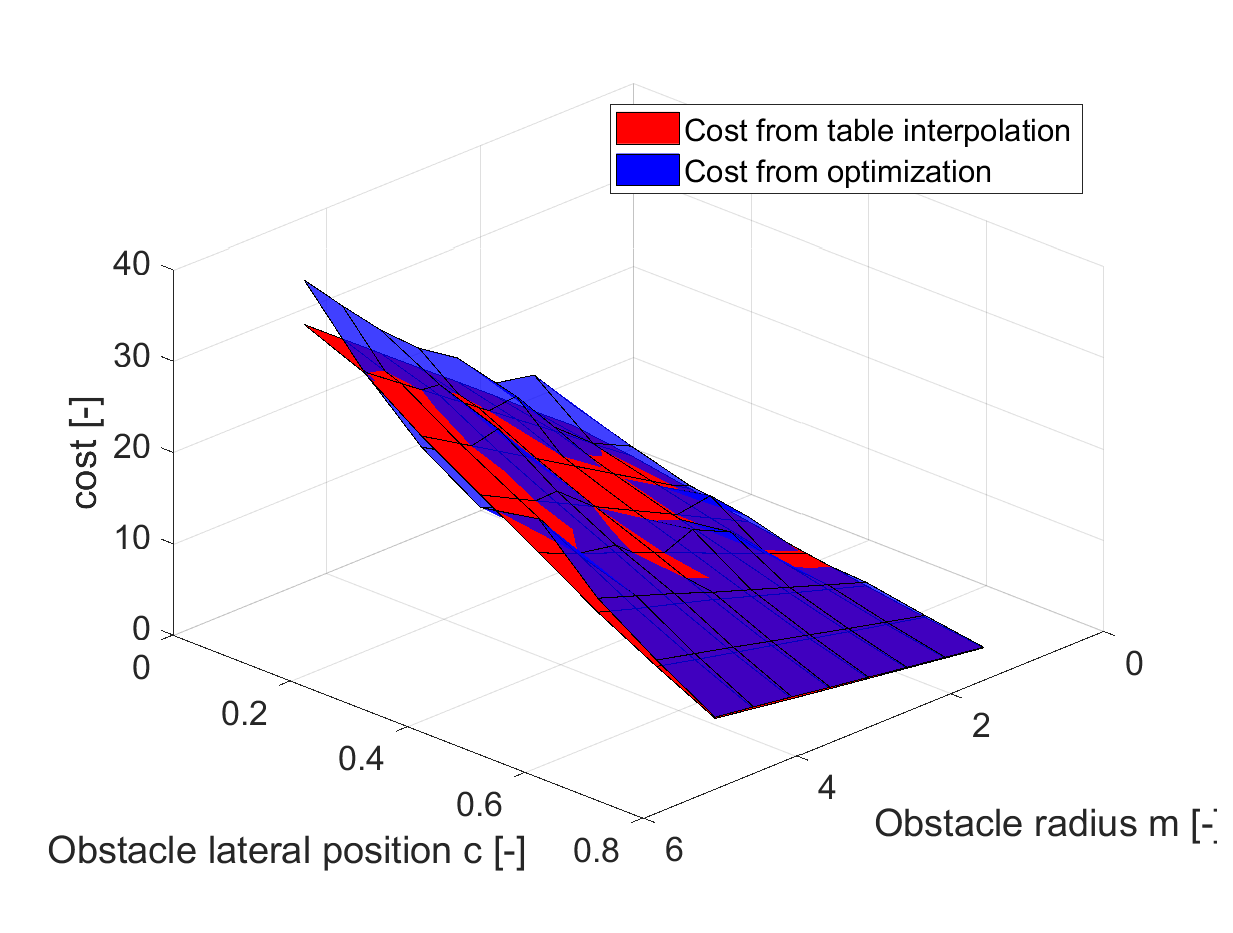
\includegraphics[width=12cm]{PaperFigures/Methods/LookupTable/costPlanes}
	\caption{Cost of UAV Obstacle Avoidance Using Interpolated and Optimized Parameters}
	\label{fig:costplanes}
\end{figure}


GVF guidance provided a low cost avoidance that quickly returns to the planned path, however the time to reach a solution using a numerical solver for the optimized set $k$ and $H_o$ increases as the size of the obstacle increases. Failure to reach a solution in adequate time may result in the UAV violating the no-fly zone or colliding with the obstacle. Lookup tables were constructed for both circulation weight $H_o$ and obstacle decay radius $k$ that were be referenced with minimal computation time compared to a single numerical optimization solution. The obstacles configuration, radius and lateral position, were non-dimensionalized by expressing said parameters in multiplicative factors of the UAV's turning radius. Non-dimensionalizing the obstacles configuration allows for a single lookup table to be used for multiple UAV velocities. 




\section{Phase III: Flight tests}
\textbf{The objective of Phase III was to demonstrate the optimized gradient vector field guidance presented in Phase II on multirotor UAV flying with fixed wing turn-rate constraints.} An overview of the experimental setup will be given for both the hardware and software that was implemented to achieve GVF guidance on a Crazyflie quadcopter. Python and MATLAB GVF guidances are compared to confirm that they are equivalent.

\subsection{Experimental Overview}
All of the scenarios discussed using GVF guidance have involved simulating a fixed wing UAV modeled as a Dubin's vehicle. The micro quadcopter shown in Figure \ref{fig:crazyflie2} was used in place of a fixed wing UAV for experimental flight tests. There are several reasons why using an indoor quadcopter is advantageous for experimental flight tests. First, finding an airspace to safely test the guidance system with an adequate clearing for takeoff and landing can be difficult. Many environmental complications such as high winds, precipitation, and low visibility could delay or prevent flight tests all together.  Flying indoors allows for more repeatable experimentation, environmental control, and use of high speed motion capture systems to provide position information to guidance and control systems without the complications of outdoor flight. 



\begin{figure}
	\centering
	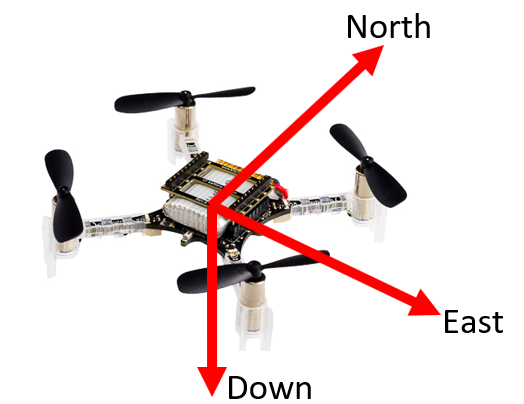
\includegraphics[trim=0 0 0 0,clip,width=7cm]{PaperFigures/methods/crazyflieNED}
	\caption{Micro Quadcopter Crazyflie 2.0 by Bitcraze}
	\label{fig:crazyflie2}
\end{figure}


The micro quadcopter, Crazyflie 2.0, designed by Bitcraze was selected as the experimental flight vehicle due to its low cost and the ability to send the vehicle roll angle, pitch angle, yaw rate, and thrust percentage commands directly over radio. The control messages can be sent through the object oriented and scripted language Python, a language with syntax very similar to MATLAB. The UAV was viewed by 8 vicon vero cameras that detect infrared light reflected by small markers placed on the vehicle. Video captured by the cameras at 100Hz is sent to a PC with a software package that estimates the pose of the vehicle and sends that information over a local area network (LAN) to a ground station PC where guidance and control calculations are made. The command messages are then sent over radio to the Crazyflie where an on-board controller accepts the commands and outputs the necessary motor output to achieve the commands. A high level overview of the experimental framework described is shown in Figure \ref{fig:experimentalFramework}. Each component of the framework will be discussed in more detail in the proceeding sections. 

\begin{figure}
	\centering
	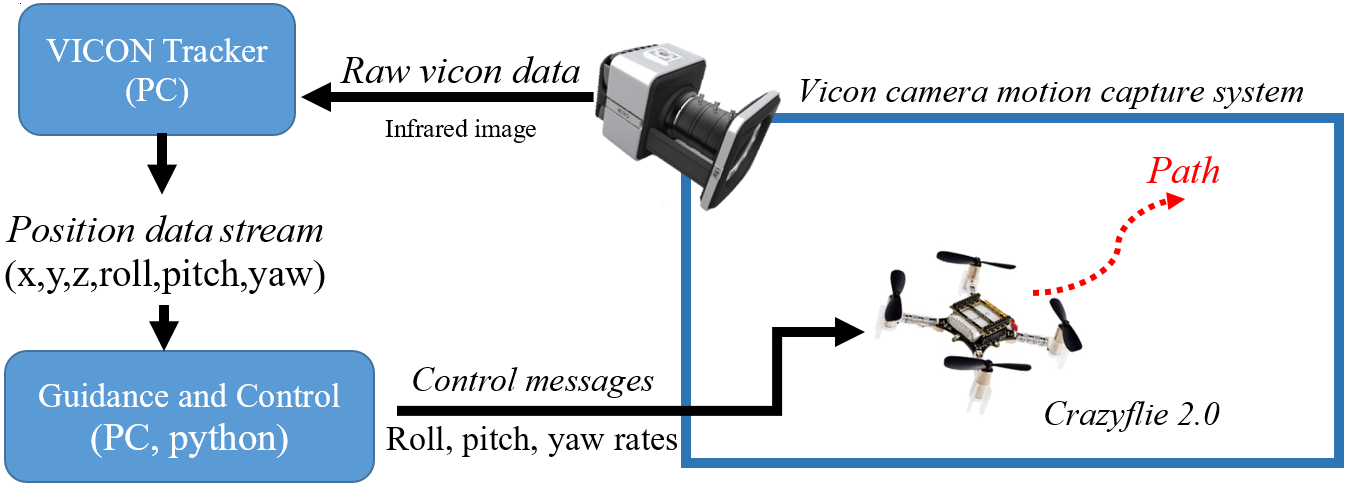
\includegraphics[trim=0 0 0 0,clip,width=15cm]{PaperFigures/Methods/experimentalSetup}
	\caption{Indoor Quadcopter Flight Experimental Layout}
	\label{fig:experimentalFramework}
\end{figure}

\subsection{Crazyflie 2.0}
The crazieflie 2.0 is a lightweight micro-quadcopter UAV weighing in at 27 grams and has an approximate payload capacity of 10 grams. On-board flight controller maintains vehicle stability by estimating it's attitude and making corrections to the four brushed motors. The software package, cfClient, interfaces with the Crazyflie to accept and transmits these control messages over radio. 


\begin{figure}[H]
	\centering
	\includegraphics[trim=0 0 0 0,clip,width=12cm]{PaperFigures/Methods/cfClient}
	\caption{Crazieflie Client Radio Communication Software}
	\label{fig:cfClient}
\end{figure}

The guidance and control software that calculates these command messages was hosted on a remote machine and not on-board the UAV, primarily for the convenience of fast development. The guidance and control was written in Python, which is highly portable and could easily be implemented on-board a UAV. 


\subsection{Python Guidance and Control Ground Station}
The guidance and control framework developed for experimentation resembles that described in Figure \ref{fig:autopilotloops}. Navigation script taps into a stream of data provided by the Vicon tracker software and distributes that data to guidance and control algorithms. Position $(x,y,z)$ and yaw $\phi$ are provided to the control algorithm which consists of four PID controllers. The UAV was set to fly at constant altitude for all simulations and experimentation, therefore only planar position $(x,y)$ were provided to the guidance system. Heading guidance from the optimized GVF was converted to a carrot located at a position $(xc,yc)$ is sent to the control system to be used as set-points. Control messages are relayed to a radio interface software, cfClient, which communicates the control messages with the Crazyflie. An overview of the described system is shown in Figure \ref{fig:cfControlClass}.

\begin{figure}[H]
	\centering
	\includegraphics[trim=0 0 1 0,clip,width=14cm]{PaperFigures/Methods/cfControlClass}
	\caption{Crazyflie Guidance and Control Software Framework}
	\label{fig:cfControlClass}
\end{figure}

The control algorithm consists of four PID controllers which are used to calculate roll rate, pitch rate, yaw, and thrust to drive the UAV to a desired setpoint. The error is measured by subtracting the measured state $(x,y,z,yaw)$ from the desired setpoint. The block diagram of the PID controller is shown in Figure \ref{fig:pid}. Gains P, I, and D for each controller is tabulated in Table \ref{table:pidGains} below. 

\begin{figure}[H]
	\centering
	\includegraphics[trim=0 0 0 0,clip,width=14cm]{PaperFigures/Methods/pid}
	\caption{Crazyflie Guidance and Control Software Framework}
	\label{fig:pid}
\end{figure}

\begin{table}[H]
	\centering
	\caption{Tuned PID Gains for Roll, Pitch, Yaw Rate, and Thrust Controller}
	\label{table:pidGains}
	\begin{tabular}{|c|c|c|c|}
		\hline 
		Control Parameter & P & I & D \\ 
		\hline 
		Roll Angle & 29 & 2.5 & 19 \\ 
		\hline 
		Pitch Angle & 29 & 2.5 & 19 \\ 
		\hline 
		Yaw Rate & 80 & 50 & 30 \\ 
		\hline 
		Thrust Percentage & 100 & 90 & 70 \\ 
		\hline 
	\end{tabular}
\end{table}
 
Applying the Dubin's fixed turn rate constraints was accomplished by saturation control. The current heading of the UAV, $\theta$ was determined from the velocity vector of the Crazyflie. The commanded heading from the optimized GVF was limited such that the change in heading was no greater than $\dot{\theta}$, in this case 20  degrees  per  second.
 
 \section{Python Guidance Validation}

The optimized GVF guidance developed in MATLAB in Phases I and II was programmed into Python and compared under several scenarios to ensure that the guidance produced were identical. First, a path following GVF was calculated in Python for a straight line and results overlaid with an identical scenario in MATLAB. The quiver plots show guidance calculated by MATLAB aligning with the guidance calculated in Python shown in Figure \ref{fig:valPythonStraightPath}.

\begin{figure}[H]
	\centering
	\includegraphics[trim=0 150 0 150,clip,width=10cm]{PaperFigures/Methods/resultsPython/PathConfirm}
	\caption{Validation of Python Straight Path Guidance Overlaid with MATLAB}
	\label{fig:valPythonStraightPath}
\end{figure}



Summing an avoidance path with the path following field with no circulation results in the guidance shown in Figure \ref{fig:valPythonSummed}.



\begin{figure}[H]
	\centering
	\includegraphics[trim=0 140 0 140,clip,width=10cm]{PaperFigures/Methods/resultsPython/summedFields}
	\caption{Validation of Python Summed Guidance Overlaid with MATLAB}
	\label{fig:valPythonSummed}
\end{figure}

Lastly, the Python guidance was simulated with an identical Dubins vehicle as MATLAB and shown to have identical paths in Figure \ref{fig:pythonMATDubins}


\begin{figure}[H]
	\centering
	\includegraphics[trim=0 240 0 260,clip,width=16cm]{PaperFigures/Methods/resultsPython/dubinsPaths}
	\caption{Validation of Python Dubins UAV Route Overlaid with MATLAB}
	\label{fig:pythonMATDubins}
\end{figure}

Additional validation quiver plots with the obstacle field, decay field, and circulation in a obstacle field can be found in the appendix. 


\section{Summary of Methodology}

Equations for path following and obstacle vector field guidance were presented. Singularities in a summed field were discussed and a method for locating them numerically was provided. The fixed wing UAV modeled as a Dubin's vehicle with fixed turn rate constraint was guided by a path following guidance to converge and follow a straight line. Obstacles were defined in terms of UAV turning radius for convenience and the obstacle field summed with path following field. Cost functions for evaluating the performance of obstacle avoidance in terms of path deviation was provided. Paths with strictly repulsive guidance were shown to guide the UAV away from the obstacle but with excess path deviation, unnecessary turns, and slow path convergence. Adding circulation to the obstacle field improved performance and reduced the overall cost. A large space of circulation and decay multipliers were evaluated and the cost displayed in a heatmap. The combination of parameters that provide the least cost guidance can be selected to provide an optimized guidance, however takes significant computation time to evaluate the large parameter space. A numerical method for determining parameters was presented and an example of it's execution provided. Lastly, the optimized GVF guidance was implemented into python to be used for real-time obstacle avoidance guidance for the Crazyflie quadcopter. Next, results for each phase will be discussed. 


\chapter{Results}
\section{Introduction to Results}

The singularity detection method discussed in Phase I and optimized path following and obstacle avoidance guidance presented in Phase II were demonstrated in four scenarios. Both path centered and off-centered obstacles of various radii are evaluated with a simulated fixed wing UAV. The optimized GVF circulation $H_o$, decay radius multiplier $k$, and path deviation cost $\bar{\gamma}$ is documented for each scenario. The optimized GVF guidance implemented on a Crazyflie quadcopter is then used in four scenarios consisting of centered, off-centered, and various radii obstacles. Path deviation cost for experimental flights and simulation are compared for their percent difference in cost.


\section{Phase I \& II}

The methods discussed in Phase I and Phase II for detecting singularities in a summed GVF and optimizing obstacle field decay radius and circulation will now be demonstrated for several scenarios involving a Dubin's vehicle modeling a fixed wing with turn rate constraints. Avoidance scenarios that represent the possible configurations of an obstacle that lies along a pre-planned path consist of small obstacles, large obstacles, path centered obstacles, and path offset obstacles. small obstacles are considered those with radius $r_o = \theta_r$ while large obstacles have a radius $r_o\ge5\theta_r$. Centered obstacles represent the worst case avoidance scenario where the UAV must deviate at least $50\%$ of the obstacle's radius in order to successfully avoid. Counterclockwise and clockwise avoidance have identical costs for the path centered obstacle since the routes determined from the optimizer are symmetric. In the centered obstacle scenarios presented, it is assumed that clockwise avoidance is desired and the initial conditions and bounds were set accordingly. Table \ref{table:avoidanceScenarios} lists four avoidance avoidance scenarios that were evaluated.


\begin{table}[]
	\centering
	\caption{GVF Avoidance Scenarios}
	\label{table:avoidanceScenarios}
	\begin{tabular}{|l|c|c|}
		\hline
		\multicolumn{1}{|c|}{Scenario Number} & Obstacle radius multiplier m & Obstacle lateral position $y_o$    \\ \hline
		1                                     & 1 & 0     \\ \hline
		2                                     & 5 & 0     \\ \hline
		3                                     & 1 & $0.5r_o$ \\ \hline
		4                                     & 5 & $0.5r_o$ \\ \hline
	\end{tabular}
\end{table}

\section{Worst Case Avoidance Scenario}
A worst case avoidance scenario will be used to compare the optimized GVF with waypoint, VFF, and the optimal path with respect to the path deviation cost function. A circular obstacle centered on the path, $y_o = 0$, requires a deviation from the path of at least $50\% $ of the obstacles radius. A fixed wing UAV at an initial position $(-400,0)$ and heading $\theta=0^\circ$ follows the straight path connecting the points $(-400,0)$ and $(400,0)$ respectively. Traveling at a constant speed $u=25 m/s$ and with a fixed turn rate of $\dot{\theta}=20 deg/s$ the UAV must avoid an obstacle with radius $2\theta_r$ located at the origin $(0,0)$. The VFF guidance from \cite{borenstein_real-time_1990} is used with an obstacle window radius of $\theta_r+r_o$, a cell repulsion $Fr=-3$, attraction force $F_t=0.8$, range exponent $n=2$, and a goal located at $(700,0)$. For LOS waypoint guidance, $7$ waypoints with a small waypoint radius of $10m$ was chosen. Each diversion waypoint added drives the guidance closer to optimal, however has diminishing returns past $6-7$ waypoints. GVF guidance with a circular repulsive field was assigned a convergence weight $G=-1$ and circulation and decay radius coefficient $k$ were determined by evaluating the cost function in Equation \ref{eq:staticCost} with initial conditions $k_i = 2$ and $H=2$. The GVF solution was bounded such that $2\leq k\leq 4$ and $1\leq H\leq 6$.  Minimizing the cost function resulted in a decay radius coefficient $k=2.78$ and a circulation value $H=1.88$. The Dubin's paths for the three guidance methods discussed is shown in Figure \ref{fig:comparemethods}. \\

VFF results in a UAV route that has excess deviation from the planned path with excessive turns. Waypoint guidance returns to the path more quickly than VFF, however deviates from the planned path farther then necessary. GVF leaves the path before waypoint guidance and tracks the outside of the obstacle closely and then quickly converges back to the pre-planned path. The cost of each method, defined in Equation \ref{eq:staticCost}, is displayed in the bar plot shown in Figure \ref{fig:barplotperformance}.


\begin{figure}[H]
	\centering
	\includegraphics[trim=0 50 0 65,clip,width=15cm]{Figures/Simulations/compareMethods}
	\caption{Path of UAV Guided by Guidance Methods}
	\label{fig:comparemethods}
\end{figure}


\begin{figure}[H]
	\centering
	\label{fig:barPlotCost}
	\includegraphics[width=15cm]{Figures/Simulations/barPlotPerformance}
	\caption{Cost Performance for Various UAV Guidance Methods}
	\label{fig:barplotperformance}
\end{figure}

Gradient vector field for path following and circular obstacle avoidance was optimized and shown to have similar performance to waypoint avoidance without the need to re-plan the mission path. The obstacle avoidance GVF acts on the same principle as VFF, however guidance vectors are given circulation which aid in returning the UAV back to the planned path without intervention. 


\section{Four Avoidance Scenarios}
For each scenario a fixed wing UAV is assumed to be following a pre-planned path traveling at constant speed $u=15m/s$ with a turnrate $\dot{\theta}=20 deg/s$. The UAV's initial position is set to $(100m,0)$ and heading $\theta = 180^\circ$, where $m$ represents the obstacles radius multiplier. Each scenario tabulated in Table \ref{table:avoidanceScenarios} are discussed and obstacle GVF decay radius, circulation, and cost are summarized.\\

Scenario 1 consists of a path centered obstacle with a radius equal to that of the UAV's turning radius $\theta_r$. Minimizing the path deviation cost function  $\bar{\gamma}$ in Phase II results in a route that avoids the obstacle and quickly returns to the planned path. The total cost of scenario 1 for avoiding the obstacle is $\bar{\gamma}=7$ for decay radius multiplier $k=2.8$ and circulation $H_o = 2.1$, shown in Figure \ref{fig:m1y0solved}. A single singularity is found from searching for solutions to the singularity condition defined in Equation \ref{eq:singularityCondition} in Phase I. The singularity is removed from the UAVs route through the addition of circulation, as discussed in Phase I.

\begin{figure}[H]
	\centering
	\includegraphics[trim = 0 85 0 85, clip, width=16cm]{Figures/results/m1Y0Solved}
	\caption{Centered Obstacle With Small Radius Avoided by Dubin's UAV in Simulation}
	\label{fig:m1y0solved}
\end{figure}

Scenario 2 consists of a path centered obstacle with a radius equal to that of 5 times the UAV's turning radius $\theta_r$. The total cost of scenario 2 for avoiding the obstacle is $\bar{\gamma}=37$ for decay radius multiplier $k=2.8$ and circulation $H = 2.1$, shown in Figure \ref{fig:m1y0solved}. A single singularity is detected on the radius of equal strength, however does not lie along the UAVs path.


\begin{figure}[H]
	\centering
	\includegraphics[trim = 0 85 0 85, clip, width=16cm]{Figures/results/m5Y0Solved}
	\caption{Centered Obstacle with Large Radius Avoided by Dubin's UAV in Simulation}
	\label{fig:m5y0solved}
\end{figure}

Scenario 3 consists of a path off centered obstacle with a radius equal to that of the UAV's turning radius $\theta_r$. The shortest direction around the obstacle can be determined from inspection, therefore negative circulation conditions and bounds are given to the minimizer to produce the guidance shown in Figure \ref{fig:m1y05} for counterclockwise circumnavigation. The total cost of scenario 3 for avoiding the obstacle is $\bar{\gamma}=3$ for decay radius multiplier $k=2.4$ and circulation $H_o = -2.6$.



\begin{figure}[H]
	\centering
	\includegraphics[trim = 0 85 0 85, clip, width=16cm]{Figures/results/m1Y05}
	\caption{Off Centered Obstacle with Small Radius Avoided by Dubin's UAV in Simulation}
	\label{fig:m1y05}
\end{figure}

Scenario 4 consists of a path off centered obstacle with a radius equal to 5 times that of the UAV's turning radius $\theta_r$. Again, the shortest direction around the obstacle is determined from inspection. The total cost of scenario 4 for avoiding the obstacle is $\bar{\gamma}=14$ for decay radius multiplier $k=2.4$ and circulation $H_o = -2.7$.


\begin{figure}[H]
	\centering
	\includegraphics[trim = 0 85 0 85, clip, width=16cm]{Figures/results/m5Y05}
	\caption{Off Centered Obstacle with Large Radius Avoided by Dubin's UAV in Simulation}
	\label{fig:m5y05}
\end{figure}


Scenarios involving both path centered and off centered obstacles of various radii were investigated. For each simulation a UAV traveling along the path is guided around an obstacle and then back to the planned path without violating the obstacle, traveling through or near singularities, and without excess path deviation. The optimized GVF was then implemented on a Crazyflie 2.0 quadcopter flying under fixed wing turn rate constraints. 



\section{Phase III}

The optimized GVF guidance was used to guide a turn rate constrained Crazyflie 2.0 along a path and around a virtual obstacle that lied along the planned path. Several obstacle avoidance scenarios consisting of path centered, off centered, and multiple radii obstacles were conducted using the GVF guidance. The four avoidance scenarios tested are summarized in Table \ref{table:flightScenarios}. Due to space limitations, obstacles larger than $1.5 \theta_r$ were not considered. Each scenario is presented followed by a vector quiver plot containing both simulation and experimental UAV flight route. For the first scenario, both speed and PID controller response plots will be discussed. Speed and controller response plots for scenarios 2,3 and 4 can be found in the appendix. 


\begin{table}[H]
	\centering
	\caption{Experimental Scenarios Conducted for Crazyflie Quadcopter}
	\label{table:flightScenarios}
	\begin{tabular}{|c|c|c|c|c|}
		\hline
		Scenario Number & Obstacle radius multiplier m   & Obstacle lateral position$y_o$             & k   & $H_o$ \\ \hline
		1               & 1   & 0              & 2.2 & 2.9   \\ \hline
		2               & 1   & $0.5 \theta_r$ & 2.0 & -4.6  \\ \hline
		3               & 1.5 & 0              & 2.4 & 2.7   \\ \hline
		4               & 1.5 & $0.5 \theta_r$ & 2.1 & -3.5  \\ \hline
	\end{tabular}
\end{table}


Scenario 1 consisted of a quadcopter placed at initial conditions $(-2,0) \ m$ along a pre-planned path and traveled at a mean speed of $0.15 m/s$. An obstacle of radius $r_o = \theta_r$ was avoided by summing a repulsive obstacle GVF with the path following GVF. Cost for the simulated Dubin's UAV was $\bar{\gamma} = 7.6$ and experimental flight $\bar{\gamma} = 10.3$, a $31 \%$ difference. The experimental UAV avoids the obstacle and returns to the pre-planned path, exhibiting a similar flight path as the simulated UAV. The route of the experimental flight and simulation are found in Figure \ref{fig:1Quiver} below.

\begin{figure}[H]
	\centering
	\includegraphics[trim = 50 300 0 285, clip, width=16.5cm]{Figures/results/compareFigures/1Quiver}
	\caption{Simulated and Experimental UAV Routes for Path Centered Obstacle with Small Radius}
	\label{fig:1Quiver}
\end{figure}

The most likely reason for the difference between simulation and experimental cost is the lack of a velocity controller. Carrot chasing set-points does not guarantee that a fixed speed $u$ can be maintained, even if the set-points are of equal distance away from the UAV. Additionally, in order to properly apply the Dubin's constraints of allowing finite changes in the UAVs heading, an accurate measurement of the current heading is necessary. Heading is estimated from the numerical derivative of the UAV's position at the current and last time step $t$, $t-1$, and time between updates $dt$. Due to both measurement and process noise from Vicon and the inherent instability of quadcopters respectively, measuring the state at lower speeds had significant uncertainty. The estimated speed from the numerical derivative of position is shown in Figure \ref{fig:1u} below. The mean path following speed is the mean of the speed estimates ranging from the start to the end of path following and obstacle avoidance. Takeoff and landing speeds prior to path following were not included when calculating the  mean speed. 


\begin{figure}[H]
	\centering
	\includegraphics[trim = 0 150 0 200, clip, width=12cm]{Figures/results/compareFigures/1u}
	\caption{UAV Speed Versus Time During Flight Experiment of Scenario 1}
	\label{fig:1u}
\end{figure}


The planar position states $x$ ,$y$, altitude $z$, and yaw rate for scenario was is shown in Figure \ref{fig:1Controller}. The PID controllers were sent planar carrot set-points based on the GVF guidance, shown in red, and the state response measured with Vicon is shown in blue. 

\begin{figure}[H]
	\centering
	\includegraphics[trim = 65 200 0 200, clip, width=17cm]{Figures/results/compareFigures/1Controller}
	\caption{State Response Plots for Scenario 1}
	\label{fig:1Controller}
\end{figure}



Scenario 2 consisted of a quadcopter placed at initial conditions $(-2,0) meters$ along a pre-planned path and traveled at a mean speed of $0.16 m/s$. An obstacle of radius $r_o = \theta_r$ and lateral position $y_o=0.5 \theta_r$ was avoided by summing a repulsive obstacle GVF with the path following GVF. Cost for the simulated Dubin's UAV was $\bar{\gamma} = 3.6$ and experimental flight $\bar{\gamma} = 5.0$, a $32 \%$ difference. The experimental UAV avoids the obstacle and returns to the pre-planned path, exhibiting a similar flight path as the simulated UAV. The route of the experimental flight and simulation are found in Figure \ref{fig:2Quiver} below. The combination of the path following and obstacle fields did not result in any GVF singularities in this scenario. 

\begin{figure}[H]
	\centering
	\includegraphics[trim = 50 300 0 285, clip, width=16.5cm]{Figures/results/compareFigures/2Quiver}
	\caption{Simulated and Experimental UAV Routes for Off Centered Obstacle with Small Radius}
	\label{fig:2Quiver}
	\end{figure}

Scenario 3 consisted of a quadcopter placed at initial conditions $(-2,0) meters$ along a pre-planned path and traveled at a mean speed of $0.16 m/s$. An obstacle of radius $r_o = 1.5 \theta_r$ and lateral position $y_o=0$ was avoided by summing a repulsive obstacle GVF with the path following GVF. Cost for the simulated Dubin's UAV was $\bar{\gamma} = 13.4$ and experimental flight $\bar{\gamma} = 13.7$, a $2.5 \%$ difference. The experimental UAV avoids the obstacle and returns to the pre-planned path, exhibiting a similar flight path as the simulated UAV. The route of the experimental flight and simulation are found in Figure \ref{fig:3Quiver} below. 


\begin{figure}[H]
	\centering
	\includegraphics[trim = 50 250 0 250, clip, width=16.5cm]{Figures/results/compareFigures/3Quiver}
	\caption{Simulated and Experimental UAV Routes for Path Centered Obstacle with Large Radius}
	\label{fig:3Quiver}
\end{figure}

Scenario 4 consisted of a quadcopter placed at initial conditions $(-2,0) meters$ along a pre-planned path and traveled at a mean speed of $0.14 m/s$. An obstacle of radius $r_o = 1.5 \theta_r$ and lateral position $y_o=0.5r_o$ was avoided by summing a repulsive obstacle GVF with the path following GVF. Cost for the simulated Dubin's UAV was $\bar{\gamma} = 5.2$ and experimental flight $\bar{\gamma} = 9.2$, a $56 \%$ difference. The experimental UAV avoids the obstacle and returns to the pre-planned path, exhibiting a similar flight path as the simulated UAV. The route of the experimental flight and simulation are found in Figure \ref{fig:4Quiver} below. 


\begin{figure}[H]
	\centering
	\includegraphics[trim = 50 275 0 250, clip, width=16.5cm]{Figures/results/compareFigures/4Quiver}
	\caption{Simulated and Experimental UAV Routes for Off Centered Obstacle with Large Radius}
	\label{fig:4Quiver}
\end{figure}

A summary of the scenarios tested and the cost associated with each simulation and flight test are shown in Table \ref{table:compareResults} below. 

\begin{table}[H]
	\centering
	\caption{Simulation and Experimental Cost Comparison Table for Scenarios 1-4}
	\label{table:compareResults}
	\begin{tabular}{|c|L{3cm}|L{3cm}|L{2.5cm}|L{2.5cm}|}
		\hline
		Scenario & Simulation Cost & Experiment Cost & Cost \% Difference & Mean Experiment Velocity [m/s] \\ \hline
		1               & 7.6                                  & 10.3                                 & 31                                      & 0.15+-0.1                                     \\ \hline
		2               & 3.6                                  & 5.0                                  & 32                                      & 0.16 +- 0.1                                   \\ \hline
		3               & 13.4                                 & 13.7                                 & 2.5                                     & 0.16+-0.1                                     \\ \hline
		4               & 5.2                                  & 9.2                                  & 56                                      & 0.14 +- 0.1                                   \\ \hline
	\end{tabular}
\end{table}


\section{Summary of results}

An optimized GVF for path following and obstacle avoidance with singularities removed from the UAV's path was presented. Singularities in the summed GVF were detected numerically by searching for the location of null magnitude vectors in the summed field with initial conditions placed on the radius of equal strength. Decay radius and circulation weights were determined by minimizing a cost function that penalizes the UAV for deviating from the path and violating the obstacle's space. The optimized GVF was simulated for a fixed wing UAV under various scenarios consisting of path centered, off centered, and multiple radii obstacles. Experimental flight tests were conducted with a Crazyflie 2.0 quadcopter with fixed wing constraints and the flight path cost was compared against that of simulation. 

\chapter{Conclusions}

A GVF for path following and circular obstacle avoidance was optimized and shown to have similar performance to waypoint avoidance with the benefits of VFF. The obstacle avoidance GVF acts on the same principle as VFF, however guidance vectors are given circulation which aid in guiding the UAV back to the planned path without intervention. Singularities in summed GVFs were identified by numerically finding locations where GVF magnitudes were null in a summed field. It was shown that optimizing circulation and decay radius of a repulsive GVF removed singularities from a UAVs path and reduced path deviation cost function compared to VFF. Lookup tables for both circulation and decay radius were constructed for a range of obstacle configurations which can be used real time. The optimized avoidance was then used to guide a multirotor UAV in several avoidance scenarios. Contributions from each phase is summarized below. \\

\textbf{The objective of Phase I was to characterize and present a method of locating singularities in a summed GVF.}
Attractive path following and repulsive GVF guidance for avoiding circular obstacles along a planned path was achieved by modifying a circular GVF's decay radius, convergence, and circulation weights. Summing the attractive and repulsive GVFs was shown to result in guidance that directs the UAV along the planned path while directing away from the obstacle. Regions in the summed guidance where the path following and obstacle guidance directly oppose each other can result in vectors of zero length, called singularities. The location of singularities were predicted to be along the radius of equal strength, where both fields have equal vector magnitudes. The location of singularities were determined by numerically solving for the location of vectors with null magnitude with initial conditions placed around the radius of equal strength.




\textbf{The objective of Phase II was to determine a combination of circulation and decay radius for a circular obstacle GVF that produces an optimized obstacle avoidance.} It was shown that equating the path’s circulation weight to that of the UAV’s speed provides a balance between rise time and overshoot when converging and following a path. A Repulsive GVF was added to the path following GVF and an array of decay radii and circulation weights were evaluated for their path deviation costs in simulation for a worst case head on collision scenario. The minimal cost from a configuration search could be used to provide an optimal guidance, however evaluating a large array of parameters takes significant time and may be unique to each obstacle size, position, and UAV characteristics. An optimization problem was described and a method of solving for GVF circulation and decay weight with reduced computation time was presented. Optimizing GVF parameters real-time is problematic for large obstacles because computation time increases as the obstacle's radius increases. Pre-computing possible obstacle configurations and storing circulation and decay radius into a lookup table was shown to provide similar performance to optimization alone.\\

\textbf{The objective of Phase III was to demonstrate optimized GVF guidance on multirotor UAV flying with fixed wing turn-rate constraints.} The optimized GVF for path following and obstacle avoidance was implemented on a Crazyflie 2.0 quadcopter for real time guidance while flying under fixed wing constraints. Several path following and circular obstacle avoidance scenarios were tested consisting of path centered, off center, and multiple radii obstacles. Flight test and simulation flight routes were compared for both their general behavior and costs. The quadcopter followed the same general path as the simulated UAV, however had an average of $30 \%$ higher cost compared to the simulated path. The difference in cost is attributed to both the lack of a velocity controller and the high process and measurement noise when measuring the UAV’s velocity.  \\


UAVs typically rely on path planning algorithms to provide an obstacle free and flyable path prior to flight. In the event that unplanned obstacles are encountered a new path may have to be generated which may not be possible if communication with a ground station is lost. Path following and obstacle avoidance was achieved without the need to re-plan the mission path by using optimized GVF decay radius and circulation parameters. Simulations were conducted with a fixed wing UAV modeled as a Dubin's vehicle using the GVF guidance and circulation and decay radius were selected which minimized a path deviation cost function. Singularities in the GVF were characterized and located numerically. The optimized GVF guidance was implemented in an indoor quadcopter with turn-rate constraints to emulate a fixed wing UAV. Results comparing simulations and indoor flight tests were compared. \\

Guidance for path following and obstacle avoidance without the need to re-plan mission paths has the potential to aid in increasing unmanned systems autonomy. Obstacles can be avoided without the intervention of a human operator and they can do so at minimal deviation from the planned path. Planned paths represent a route in which a task must be completed, therefore, maintaining a low lateral error with respect to the path increases the UAVs overall effectiveness.



\bibliographystyle{aiaa}   
\bibliography{bib}


\appendix
\chapter{Methodology Phase I}

The figures herein depict the effects of GVF normalization for both convergence $\overrightarrow{V}_{conv}$ and circulation $\overrightarrow{V}_{circ}$ components of a circular field as well the application of the decay function $P$. The non-normalized attractive field for converging and following a circular path is shown in Figure \ref{fig:gvfCircAttractive}a. Note that the vectors decay in magnitude as they approach the target curve due to the negative definite nature of the potential function $V$ described in Equation \ref{potentialV}. Normalizing the vector $\overrightarrow{V}_conv$ produces vectors of equal length for the entire configuration space, shown in Figure \ref{fig:gvfCircAttractive}b.


\begin{figure}[H]
	\begin{subfigmatrix}{2}% number of columns
		\centering	
		\subfigure []{\includegraphics[width=7.5cm] {PaperFigures/NNcompWithoutTitles/circAttractive}}
		\subfigure []{\includegraphics[width=7.5cm] {PaperFigures/compWithoutTitles/circAttractive}}
		\hspace*{0mm}
	\end{subfigmatrix}
	\caption{GVF Circular Attractive Field without Normalization (a) and with Normalization (b)}
	\label{fig:gvfCircAttractive}
\end{figure}

Modifying the convergence weight $G$ of the vector field shown in Figure \ref{fig:gvfCircAttractive}b results in a field that directs away from the target circular path, shown in Figure \ref{fig:largerepulsive}. Note that vectors inside of the circular target path direct inwards towards a singular point, potentially leading to a trap situation. Reducing the target path's radius $r$ to that of several orders of magnitude smaller than the UAV's turning radius, $\theta_r$, results in a field that directs away from a small point shown in Figure \ref{fig:normalizedrepulsive}.

\begin{figure}[H]
	\centering
	\includegraphics[width=0.7\linewidth]{Figures/methods/largeRepulsive}
	\caption{Repulsive Circular Field with Large Radius}
	\label{fig:largerepulsive}
\end{figure}

\begin{figure}[H]
	\centering
	\includegraphics[width=0.7\linewidth]{Figures/methods/normalizedRepulsive}
	\caption{Repulsive Circular Field with Small Radius}
	\label{fig:normalizedrepulsive}
\end{figure}

Circulation vectors of GVF decay in strength as they approach the center of the circular target curve shown in Figure \ref{fig:gvfCircCirculation}a. Normalizing the vectors $\overrightarrow{V}_circ$ forces the vectors to have length unity for the entire configuration space, shown in Figure \ref{fig:gvfCircCirculation}b.

\begin{figure}[H]
	\begin{subfigmatrix}{2}% number of columns
		\centering	
		\subfigure []{\includegraphics[width=7.5cm] {PaperFigures/NNcompWithoutTitles/circCW}}
		\subfigure []{\includegraphics[width=7.5cm] {PaperFigures/compWithoutTitles/circCW}}
		\hspace*{0mm}
	\end{subfigmatrix}
	\caption{Circular GVF without Normalization (a) and with Normalization (b)}
	\label{fig:gvfCircCirculation}
\end{figure}

Applying the decay function $P$ described in Equation \ref{eq:decay} limits the range at which the repulsive GVF has influence on the total guidance. Strictly repulsive GVF limited by decay function $P$ is shown in Figure \ref{fig:decayApplied}a and equal magnitude convergence and circulation is shown in Figure \ref{fig:decayApplied}b.

\begin{figure}[H]
	\begin{subfigmatrix}{2}% number of columns
		\centering	
		\subfigure []{\includegraphics[trim=0 10 20 20,clip,width=7cm] {Figures/methods/decayApplied}}
		\subfigure []{\includegraphics[trim=0 10 20 20,clip,width=7cm] {Figures/methods/decayAppliedCirculation}}
		\hspace*{0mm}
	\end{subfigmatrix}
	\caption{Repulsive GVF a) No Circulation $H_o=0$ and b) with Circulation $H_o=1$}
	\label{fig:decayApplied}
\end{figure} 


\chapter{Methodology Phase III}

Implementing the GVF guidance used in Phase I and II required that the guidance be programmed in Python. Phase III methodology show validation for straight line path and summed GVF by overlaying guidance produced in MATLAB and Python. Below are validation figures for circulation $\overrightarrow{V}_{circ}$ and the decay function $P$ in Figures \ref{fig:valPythonAvoidance} and Figure \ref{fig:valPythonAvoidanceDecay} respectively.

\begin{figure}
	\centering
	\includegraphics[trim=0 140 0 140,clip,width=10cm]{PaperFigures/Methods/resultsPython/obstacle}
	\caption{Validation of Python Obstacle Guidance Overlaid with MATLAB}
	\label{fig:valPythonAvoidance}
\end{figure}

\begin{figure}[H]
	\centering
	\includegraphics[trim=0 140 0 140,clip,width=10cm]{PaperFigures/Methods/resultsPython/obstacleWithDecayAndCirculation}
	\caption{Validation of Python Obstacle Decay Guidance Overlaid with MATLAB}
	\label{fig:valPythonAvoidanceDecay}
\end{figure}
\chapter{Appendix - Results Phase III}

Speed, $u$, and PID controller responses for scenarios two through four conducted in Phase III are presented herein. Speed was recorded from takeoff to the end of path following. The mean speed $u$ in Table \ref{table:compareResults} was determined from the mean of speed $u$ between the start of path following to the end in path following indicated by the blue and red markers in the speed plots below. Measured state and set-point plots for each roll, pitch, yaw rate, and thrust PID controller are shown as well.

\begin{figure}[H]
	\centering
	\includegraphics[trim = 0 150 0 200, clip, width=10cm]{Figures/results/compareFigures/2u}

	\centering
	\includegraphics[trim = 65 210 0 200, clip, width=16cm]{Figures/results/compareFigures/2Controller}
	\caption{Experimental Scenario 2 UAV Speed and Controller Response}
	\label{fig:2Controller}
\end{figure}

\pagebreak
\begin{figure}[H]
	\centering
	\includegraphics[trim = 0 150 0 200, clip, width=10cm]{Figures/results/compareFigures/3u}
	
	\centering
	\includegraphics[trim = 65 210 0 200, clip, width=16cm]{Figures/results/compareFigures/3Controller}
	\caption{Experimental Scenario 3 UAV Speed and Controller Response}
	\label{fig:3Controller}
\end{figure}

\pagebreak
\begin{figure}[H]
	\centering
	\includegraphics[trim = 0 150 0 200, clip, width=10cm]{Figures/results/compareFigures/4u}
	
	\centering
	\includegraphics[trim = 65 210 0 200, clip, width=16cm]{Figures/results/compareFigures/4Controller}
	\caption{Experimental Scenario 4 UAV Speed and Controller Response}
	\label{fig:4Controller}
\end{figure}


\chapter{Optimization MATLAB source code}
The script optimizedGVF.m contains the optimization algorithm to determine optimized set of obstacle field decay radius $k$ and circulation $H_o$. Inputs are the UAVs initial state, constant speed $u$, and the obstacles configuration.  
\lstinputlisting{optimizedGVF.m}
\chapter{Vector Field Construction source code}
The MATLAB class vectorField.m manages the creation, summation, and plotting of GVF guidance. Instructions on how to use the class are provided in the comments above the class definition. Usage of the class is also shown in optimizationGVF.m script.

\lstinputlisting{vectorField.m}
\end{document}
